

Very soon, web-based simulation frameworks will support high fidelity simulations of what happens when agents interact with real software (and even with the people that use that software). If widely used, then those tools could become a breeding ground for malicious bots that (a) monitor a site; (b) learn its patterns; (c) exploit those patterns to slip in and cause harm.  So how to avoid that bot-apocalypse? The answer lies in point (b) above, which was “learn its patterns”. The central insight of this research is that “superfluous search” (a variant of that search-based methods, described below) can generate an army of defenders that can fend off adversaries. This army holds thousands of agents that achieve the goals of a site, but in wildly different ways. When faced with such variety, in-coming adversaries cannot find the patterns needed to attack a site. Currently we address that problem via a supervised method that knows the kinds of attacks that are currently in progress. Such supervised methods are not ideal since, in practice, a defender can be attacked by arbitrary assailants.  Hence, we propose unsupervised model selection for superfluous search.   
BACKGROUND AND MOTIVATION:  As internet-agent-engineering gets easier and easier, such malicious bots will become more and more common.  How to defend against this bot apocalypse?
      Analysts in many domains are using machine learners to tame the 21st century data explosion. Machine learning software explores data to find patterns. This learning software can search very large data sets since they exploit intelligent search biases that allow them to quickly prune irrelevancies. But the more we improve our data mining pipelines, the more we enable the creation of malicious bots. This is a particular problem in the case of adversarial bots. E.g. 


 
 
    

 
% \begin{wrapfigure}{r}{3in}
% \includegraphics[width=3in]{fig/search.png}
% \caption{Results of DODGE selecting options from \figPn example of Pareto frontier \cite{shu2019improved}. Objectives $f_1$ and $f_2$ are both to be minimized. $\epsilon$ value is set to 0.1. The gray dots represent the feasible solutions. The yellow dots represent the Pareto optimal solutions. }
% \label{fig:search}
% \end{wrapfigure}


 
 
  {\IT}.1 was tested on case studies taken from other 
  FGSM~\cite{goodfellow2014explaining},
BIM~\cite{KurakinGB17a},
JSMA~\cite{papernot2016limitations},
DeepFool~\cite{moosavi2016deepfool} and
Carlini\_Wagner~\cite{carlini2017towards,DBLP:conf/ccs/Carlini017}. 


  {\IT}.1 missed some important
XXX generate qnd test. premise is that we can explore a large space of classifiers very quickly.y is that even true?
timm

timm

Recent results in SE have highlighted the importance of of ``configuration'' in software engineering. 
This has lead to the development of many automatic configuration algorithms (and the aim
of this research is to check if those algorithms can automatically and quickly configure malware
detectors that can better detect adversaries). One terminological digression before continuing.  
The terms   ``configuration'' and ``hyperparameter optimziation''  
are used by SE and AI researchers (respectively)
to refer to the same process of finding good control for   software systems.
We say that `hyperparameter optimzation'' is the ``configuration'' process for selecting the control parameters of a learner. Recalling  \tbl{hyperparameters}, the configuration space for moderns learners can be very large. 


 
 TPE can One issue with {\IT}.1 was that even with TPE intelligently rejecting useless optimizations (i.e. those that did not maximize  $\frac{l(x)}{g(x)}$ 

Kernel dens 
pf \fig{hyperparameters} 

The space

The goal of the algorithm is to learn a detector of for malicious software that can be used on future examples. 

Given some base Learner1, XXXX

as said above, one way to confuse and defeat the adversary is to frequently adjust the learning such that the adversary can not learn the decision boundary. This can be done via search-based methods; specifically superfluous-search. As illustrated at right, as a hyperparameter optimizer adjusts the tuning parameter (in this case, number of trees in a random forest), there is a point where  further search is  superfluous (since there are no further performance improvements).  Normally, optimization stops at this point. 

      What we propose here is to continue optimization, deep into that superfluous space. We call this superfluous search. As shown at right,  superfluous search can automatically generate many different models, all of which have similar performance. In our approach, we (a) cache these superfluous models, then (b) at runtime, make decisions using any of the superfluous models, selected each time at random. In this way, we can confuse adversaries since this makes it harder for them to learn a  decision boundary . 

 
Many researchers report that modern software systems {\em come with a daunting number of configuration options}. For example, the number of configuration options in Apache (a popular web server) increased from 150 to more than 550 configuration options within 16 years ~\cite{xu2015hey}. Van Aken et al.~\cite{van2017automatic} also reports a similar trend. They indicate that, in over 15 years, the number of configuration options of POSTGRES and MYSQL increased by a factor of three and six, respectively. This is troubling since Xu et al.~\cite{xu2015hey} report that developers tend to ignore over 80\% of configuration options, which leaves considerable optimization potential untapped~\cite{xu2015hey}. For illustration, \tbl{hyperparameters} listed billions of configuration options just within the learner part of a malware detector. Another problem with configurable systems is the issue of 
{\em poorly chosen default configurations}. Often, it is assumed that software architects provide useful default configurations of their systems. This assumption can be very misleading. Van Aken et al. report that the default MySQL configurations in 2016 assume that it will be installed on a machine that has 160MB of RAM (which, at that time, was incorrect by, at least, an order of magnitude) ~\cite{van2017automatic}. Herodotou et al.~\cite{herodotou2011starfish} show how standard settings for text mining applications in Hadoop result in worst-case execution times. In the same vein, Jamshidi et al.~\cite{jamshidi2016uncertainty} reports for text mining applications on Apache Storm, the throughput achieved using the worst configuration is 480 times slower than the throughput achieved by the best configuration.
 
 
 
 
 Results from Configuration Research in SE
 
 Using that log, they find that 


Much recent work has note the {\em transferability} of adversarial examples between different kinds of learners. That is,
an adversarial  attacker can use its own  Learner1 to find ways to defeat a malware detector written in Learner2, even when the adversary has no knowledge of the Learner2 algorithm~\cite{papernot2016transferability}. 


 
 




DESCRIPTION OF PROPOSED PROJECT:  T
   



  
  especially when the malware provider
  uses adversarial attacks designed to fool the malware detector that
  the   some malicious input  is actually benign~\cite{wang2019security}.
  
  In response to attackers trying to fool malware detectors, some researchers have employed what we will call a {\em confusion}
  approach. 
  
 One way t
 \bi
 \item {\bf Security Problem:}
 There any many kinds of such inputs including  malicious Android applications or spam email or a pdf containing malicious code.
 \item {\bf SE solution}  {\em Configuation} methods~\cite{nair2018finding,harman2010search,nair2018data} using  {\em search-based SE}~\cite{chen2018beyond,nair16,harman2010search} to automatically learn  control parameters. 
We show below that once search-based configuration tools
 can learn   thousands of variants
 of a software system; then those variants can be used to {\em confuse} and  thwart the adversarial attacker. 
 \ei
 (Technical aside: as discussed below, {\em confusion} increases the ``complexity'' of the model~\cite{demontis2019adversarial}.XXXX)
 
 %Papernot2016TransferabilityIM
 
 
  
\section{Background}




 
 XXX ensemble done before using untuned methods~\cite{Smutz2016WhenAT,euh2020comparative} but that assume randomized selection of features and columns from which models are built. Our methods are still random, but ranteht rhat rawing fom ar adom distribution, we select features fonot of the dte but of the control parameters for the learners, also we don't select at random but guide ou selection via n ootimizer. also rather than focus on just one learner (as done with Dai et al. 2019~\cite{dai19} we explore a much larger space).
 
 Smutz \& Stavrou propose an itenreaeing varints: enseblmes focusing on ksiclassifeird prio examples. when classificationsa re msisied by oen classifie, a communit pf clasisfiers can still succesed
 
 sme examples of manual tuning. e.g.  Smutz \& Stavrou  Smutz \& Stavrou We tuned our Random Forest based classifier to provide classification performance comparable to the linear SVM classifier of Drebin. The primary item we tuned was the ratio of benign to malicious samples used in training each tree. This was necessary because there is an extreme imbalance in the benign to malicious ratio of the various training sets. We tuned the ratio for individual tree training to 2.5 benign to 1 malicious in order to match the desired false positive rate of 1% chosen by Arp et al. 
 
 Chinvale et al. [11]  in that they use the majority result of their en- sembles as ground truth for re-training of individual classifiers while we focus on identifying the specific examples where the ensemble prediction is not trustworthy. we do neigher: tuning the decision rule ins repsonetot he data.
 
from: https://pdfs.semanticscholar.org/0612/fdc261b459b0e84fe8590afd543e3fb08b94.pdf, p2
Recent work has demonstrated that the diversity in ensemble classifiers can improve malware detection rates [22], [29], [46], [47]. Few studies, however, advance practical strategies for detection of evasion attempts against these ensemble classifiers. 

 ts. 
  
  Building such systems is a three stage process:
  \bi
  \item
  feature engineering and data collection
  \item
  model learning
  \item
  model evaluation. 
  \ei
  In order to confuse attackers, various authors  have proposed stochastic variations of the first two steps.  For example Euh et al. 
  use  a random selection of low features lect DDD. 
  Khasawneh et al.~\cite{khasawneh2017rhmd} emply a range of XXXX
  
  
 


\section{Evaluation}
3) COMPARISON WITH OTHER RESEARCH
In order to verify the effectiveness of our method, we compare the research of Smutz and Stavrou [17] with the Ensamble HMD of Khasawneh et al. [22] using our dataset, and the optimum results are taken. See Table 5.
It should be pointed out that Ensamble HMD is a hardware-based detector, and our recurring experiments use
only the malware features used in this research and the offline universal detector (neural network) method in this research. Since it is soft probe we use, and some noise may also be introduced when acquiring HPC, the difference between the two experiment settings is not counted therein. As can be seen from the table, the multi-featured integrated detector used in our SMASH method has the highest accu- racy.

----------

  utilizes known detective pat- terns to verify whether a new application becomes a threat
   
   
   XXX prior work: randomize selection of features and models 
   expert knowledge and frequency analysis are adapted for relevant feature selection from the collected data set, which contributes to fast low-dimensional feature preparation, low storage usage, and fast learning. 
   
A malware detection system utilizes known detective pat- terns to verify whether a new application becomes a threat

\section{About}

Adversarial examples \citep{szegedy2013intriguing,biggio2013evasion},
inputs that are specifically designed by an
adversary to force a machine learning system to produce erroneous outputs, 
have seen significant study in
recent years.
%
This long line of research
\citep{dalvi2004adversarial,lowd2005adversarial,barreno2006can,barreno2010security,globerson2006nightmare,kolcz2009feature,barreno2010security,biggio2010multiple,vsrndic2013detection}
has recently begun seeing significant study as machine learning
becomes more widely used.
%

\section{otherStuff}
\begin{wraptable}{r}{3in} 
%\begin{table}[]\
\footnotesize
\begin{tabular}{lrrr} \hline

\rowcolor{gray!20}  &   & Model   &   \\ 
\rowcolor{gray!20}  & AWS &   Depot & Wolfarm \\ \hline
Image & 61 & 24 & 59 \\ \hline
\rowcolor{gray!20}Video & 13 & 2 & 0 \\ \hline
Natural language texts & 35 & 5 & 18 \\ \hline
\rowcolor{gray!20}Audio & 12 & 1 & 2 \\ \hline
Structured & 107 & 0 & 0 \\ \hline
\rowcolor{gray!20}Total & 228 & 3 & 79 \\ \hline
\end{tabular}
\caption{ 339 machine learning models
currently for hire at on-line Model Stores. From~\cite{xiu2019exploratory}. For 
a specific example of these models, see \fig{one}.}
\label{tbl:stats}
\end{wraptable}
Reducing such discrimination is an urgent  problem.
Machine learning methods can be packaged and executed in cloud "containers" (e.g. using tools like opendatahub.io).
Many of such containers are  available for rent, in
"Model Stores" at the \href{https://aws.amazon.com/marketplace/solutions/machinelearning/}{AWS marketplace}~\cite{amazon};
the \href{https://resources.wolframcloud.com/NeuralNetRepository}{Wolfram neural net repository}~\cite{wolfram};  and  the  \href{https://modeldepot.io}{ModelDepot}~\cite{modeldepot}
(see  \tbl{stats},  \fig{one}).  
Users rent these models along with the cloud-CPU needed
to run them. Then, they  upload their data to the cloud-based learner which  later on, delivers them a model generated by a machine learner.

The premise of this proposal is that  Model Stores are both a   problem, and a   solution, for model fairness:
\bi
\item
On the one hand, Model Store models  have no tools   for (a)~identifying or (b)~mitigating discriminatory bias. 
This is troubling since our preliminary analysis (in \tion{problem}) shows
that these models are  susceptible to issues of unfairness.
That is, using Model Stores, developers can unwittingly  unleash  models  
that are highly discriminatory. Worse yet, given the ubiquity of
the internet, these discriminatory models could be unleashed
on large sections of the general public.
\item
On the other hand, these Model Stores are also places where a model is   executed many times (i.e. when different users
rent the same model).  That is, Model Stores
are places for continuously collecting experience about different
models.   By  judiciously  applying  this experience, 
can we gradually make models fairer?
\ei
One way to use that experience in order to build fairer models is
{\em incremental learning}.
Incremental learning benefits from continuously growing input data by extending its knowledge base during the iterative model re-evaluation. This is important for users in the Model Store since they are billed by the consumed computing resources. Rather than re-training the whole model for new incoming data,  we believe that an incremental learner could make a more efficient use of the computing and memory resources, which make it a more cost-efficient choice for business users.   

Moreover, as later presented in \tion{aboutfairness}), the assurance of fairness comes with a non-trivial cost to the performance (accuracy in most cases) of the decision-making system. We consider such trade-off sub-optimal and remediable by our approach. While the existing algorithms can ensure fairness to some extent, it is not clear to business users that how could the fairness-assurance tool could be tuned so that users could e.g. set up the minimal guaranteed accuracy and maximum acceptable discrimination level for the discrimination mitigation process.


 
To optimize the cost of optimization-for-fairness, and to ensure the generation of fairer but still competent models
from Model Stores, we conjecture that:
\begin{quote}
{\bf HYPOTHESIS} : {\em
  Bias can be effectively learned, and incrementally mitigated  (via instance-based sensitively analytic tools) for better trade-off between fairness and performance}
  \end{quote}
Note that this conjecture exploits an essential property of 
Model Stores. Specifically, in such Model Stores,
we can routinely expect that there exists prior experience about adapting some models to new data. 

The rest of the paper proceeds as follows: \tion{back} describes background knowledge of this research area. \S\ref{preliminary} illustrates preliminary results of this paper, Open issues that await to be solved are stated in \S\ref{open}. The detailed research plan of this study is described in \S\ref{tion:plan}. Intellectual merits and broader impact of this research are discussed in \S\ref{sec:IM-BI}. Finally, prior results from PI Menzies's research are demonstrated in \S\ref{sec:PriorResults}.

\subsection{Challenge}\label{challenge}
Our research challenge is to outperform existing benchmarks in mitigating group discrimination by leveraging incremental learning.

Some of the specific challenges to them are listed below:
  
\bi
\item  {\bf  Data}: We will need more datasets than those that are widely-used in academia. This is important since we need to ensure our system can be broadly applicable in different cases. 
\item {\bf  Labeling}: Sometimes the collected data can be unlabelled, which is only acceptable in unsupervised or semi-supervised learning. Such cases may require us to label the data manually in order to generate ground truth.
\item  {\bf  Human opinion}: We attempt to weigh in human opinions about group discrimination into the model generation, because our system is ultimately designed to assist users in practical practice with machine learners. 
\item {\bf  Performance evaluation}: Different discrimination algorithms use different fairness measures as the training goal. To show the broader usefulness of our approach, we need to illustrate the effectiveness and robustness of our system under various evaluation measures. That is to say, we strive to build one system to compete against (and even prevail) multiple benchmarks in their own measurements,
\ei

To address these challenges, our solutions (at least some initial attempts) are:

\bi
\item  {\bf  Data}: We will explore more recent datasets from tasks such as hiring, application, etc. where some sensitive attributes (e.g. race, gender, age) are involved in the prediction process. 
\item {\bf  Labeling}: We will conduct user studies to obtain labels for our new data. Also, tools such as Mechanical Turk could also be useful to get ground truth. Moreover, a recent study of PI Menzies proposed a more efficient and cheaper way to label data. (EMBLEM)
\item  {\bf  Human opinion}: (Introduce FASTREAD) We will use human opinions to determine when to start/stop fitting the model.
\item {\bf  Performance evaluation}: We will at least use EOD and AOD (later discussed in \S\ref{tion:aboutfairness}) as our evaluation measurements. We will also use the corresponding measurements that are  used originally in the papers where our benchmark methods are proposed. 
\ei

% This rest of this proposal proposes the research
% needed to design {\IT}. Using
% examples from on-line Model Stores, we will create
% an implementation of
%  {\IT} tool that supports  {\bf match, dontmatch, transfer} \& 
% {\bf patch}. {\IT}'s heuristics
% will be learned from experiments with:
% \bi
% \item Machine
% learning using default parameters (i.e. no tuning);
% \item Machine learners optimized just for 
% predictive prowess
% (recall, false alarm, etc);
% \item 
% Machine learners optimized for {\em both}
% predictive prowess {\em and} fairness.
% \item 
% {\em Optimization-for-fairness}; i.e.
% machine learners that reuse prior tunings to
% faster optimize for  
% predictive prowess and  fairness
% (using {\bf match, dontmatch, transfer} \& 
% {\bf patch}).
% \ei

\begin{figure}
\begin{center}
\includegraphics[width=6in]{fig/store1.png}
 \end{center}
  \caption{One of the machine learning models
 for rent from on-line Model Stores. 
  From~\cite{xiu2019exploratory}.
  As shown in \tbl{stats}, this is one
  of the hundreds of machine learning
  apps currently for sale within Model Stores.}\label{fig:one}
  \end{figure}

\subsection{Evaluation}\label{evaluation}

\noindent
\tion{plan} of this proposal divides this research into nearly a dozen steps,
then offers extensive notes on the success criteria we will use to evaluate the products of each step. 
In this section, we offer some preliminary notes on how this work will be evaluated (and for full
details, see \tion{plan}).
This proposal will be  a success if:
\bi
\item 
 Models tuned via {\IT}  are ``better'' (fairer, offer predictions as 
 are as least as good)
  than otherwise.
  \item
The overhead associated with {\IT} is minimal; i.e. ``not much'' 
slower or more expensive   than learning without tuning (using off-the-shelf parameters)
\ei

 Note that this success criteria
 critically defends on  a working definition of ``not much'' and ``better''.
 To address this issue, we devote two entire sub-tasks to
 generating these definitions:
\bi
 \item
 As to ``better'', there are many ways to define fairness
 goals (see the discussion in \tion{aboutfairness})
 or the predictive prowess of  
  of machine learners including the standard measures (e.g.
  recall and false alarm, defined in \tion{hbo}).
  As  discussed in \tion{labrat}, our
  preliminary analysis of the Model Store apps is that
  they use a much wider range of evaluation criteria
  than just the standard measures of recall and false alarm. Hence, in this specific part of the research, we will work on collecting the model-specific criteria required to assess the predictive prowess of particular
  Model Store apps.
 \item
 As to ``not much '' more CPU,
 in \tion{costaware}, we described our survey   work
 where we will determine the
 ``cost awareness curves'' of ModelStore users; i.e. how much the probability of buying a Model Store app is effected by the price of that app. The ``knee'' of the curve will be used to define our CPU goals.

\ei

\subsection{Embedding Innovations in Real Systems}\label{embedding}

Our target application area are not just
the hundreds of models listed in \tbl{stats}. Rather,
our more general purpose is to assurance fairness in the thousands more
models that we anticipate   will come on-line in Model
Stores and be marketed to the general public during the period of this research.  
To enable this more general purpose,  one of  the steps in our research plan is the dissemination of these results to the managers
of Model Store and the developers of Model Store apps.
A pre-condition to that discussion would be some demonstration
that our proposed approach is not so slow that it might reduce  sales within Model Stores.
Therefore, our research plan (see \tion{package}) is 
to spend much time
carefully packaging and promoting {\IT}
to
Model Store managers and app developers
(once we obtain
  initial results showing 
 we can offer ``better'' models with ``not much'' more CPU cost).

\subsection{Transformative Research}\label{transformative}
 Our work speaks to a core issue in AI: how to trust automatically generated models.   ``Trust''  means  different  things  to  different  people  but,  at  the  very  least,  we  should demand that our AI models are not needlessly discriminating against specific social groups.
In terms of multi-disciplinary work, this research bridges the studies of
algorithms and the social sciences that study the ethical
application of technology. PI Menzies' training
(which
includes research degrees  in Cognitive Science),
is particularly suited to such
an endeavor. 
In terms of core computer science and machine learning, 
this work will
explore a potentially vast space of hyperparameters  
in order to find fairer models. While our focus here is on ``fairness'', we also note that our methods could also be used
to explore other areas where humans and computers work in partnership to explore complex problems. 
 
\subsection{Relevance  }\label{relevance} 
 
  The proposal is   relevant to the   solicitation. 
 As stated there,
 {\em AI, including ML, raises significant novel challenges around ensuring non-discrimination of decision making.   Methods to assure fairness need to be developed so that, when such methods are applied, they ensure acceptance, trustworthiness, and lack of adverse bias.} In this research, we propose
 a general method (hyperparameter optimization) to ensure that fairness.

\subsection{ Uniqueness of this Research}\label{uniqueness} 

   To the best of our knowledge, our work is the first to characterize fairness as  multi-objective problem.
  While others    have explored hyperparameter optimization~\cite{Mockus1994,hutter2011sequential,bergstra2011algorithms,hutter2010sequential,piche2009model,snoek2012practical,martinez2014bayesopt,kotthoff2017auto,chen2009efficient,lacoste2014sequential,maclaurin2015gradient,feurer2015initializing,bergstra2012random,bartz2010sequential,bergstra2013hyperopt,eggensperger2013towards,thornton2013auto,bergstra2015hyperopt,piche2010model},
  none have considered the    CPU restrictions required for
  optimization-as-fairness (i.e.  
 not much more CPU than learning without tuning).



\subsection{ Generality } \label{generaliaty}
While this proposal   focus  on    fairness and Model Stores,
{\IT} should apply whenever a machine learning pipeline is executed many times
(e.g. 
when  many people  use the  a data    ``dashboard'' to run a small number of queries, many times). To say the least, there are many such domains.


\section{Background}\label{tion:back}

\subsection{More About Model Stores}\label{tion:problem}
 
 In order to assess the potential for unfair models from Model Stores,  we sampled 32 models at random from
the AWS model store. 
That sample found many models that  that could   inappropriately target protected social groups (e.g. age, gender or race, or someone's social/financial status). For example:
\bi
\item
{\em hyScore} is an NLP tool which, amongst other things, performs  sentiment analysis of content. hyScore accepts arbitrary free form text which, potentially, could reference   social groups we might want to protect.
\item
Another model we found was 
{\em Credit Default Predictor} that uses   23 attributes include gender, education, age, and previous history of payments to generate an   predictor of the chances a customer will default on a loan
\item
Also, in our sample, we found the 
{\em Hospital Readminission} model that  predicts the probably that a patient will not be readmitted after discharge. This model's inputs include financial class, sex and age. Depending on the protected attributes a hospital may decide not to release the patient as the model shows high probability of readmission, while another patient with same other attributes but different protected attribute values can be released.
\ei
Note that these models  
were  based on a preliminary survey
of 32 of the 300+ models currently available on-line.
Based on this survey, we conclude that many of Model Store
applications could
 produce unfair models; i.e.  Model Stores need additional tools
to recognize
and mitigate
unfairness. Hence, this proposal.

\subsection{About Fairness}\label{tion:aboutfairness}
\begin{wraptable}{r}{3in}
 
\begin{tabular}{|p{2.9in}|}\hline
\rowcolor{gray!20}\small
\bi

\item
Google's sentiment analyzer model  which determines positive or negative sentiment, gives negative score to   sentences like \textit{`I am a Jew', and `I am homosexual'}\cite{Google_Sentiment}. 
\item
Facial recognition software which predicts characteristics such as gender, age from images has been
found to have a much higher error rate for dark-skinned women compared to light-skinned men \cite{Gender_Bias}. 
\item
A popular photo tagging app   assigns animal category labels to dark skinned people \cite{Google_Photo}. 
\item 
Some recidivism assessment models used by the criminal justice system         are more likely to falsely label black defendants as future criminals (at  twice the rate as white defendants) \cite{Machine_Bias}. 
\item
Amazon.com stopped using automated  recruiting  tools after finding anti-women bias\cite{Amazon_Bias}. 
% \item
% Cathy O'Neil provided even more examples of unfair decisions made by software in her book ``Weapons of Math Destruction''\cite{O'Neil:2016:WMD:3002861}. She argued that machine learning software generates models that are full of bias. Hence, this is one of the reasons their application results in unfair decisions.
\ei\\\hline
\end{tabular} 
 
\caption{Examples of Discriminatory Software.}
\label{tbl:eg}
\end{wraptable}
Machine learning software, by its nature, is always a form of statistical discrimination. 
This discrimination becomes objectionable when it places certain social groups at  a systematic advantage and other unprivileged groups at a systematic disadvantage. In some situations, such as employment (hiring and firing), discrimination is not only objectionable, but illegal.


It is timely to reflect on the implications of such discrimination.
Such software is increasingly being used to make decisions that affect people's lives and  to support decision making in high-stakes applications such as mortgage lending, hiring, and prison sentencing. 
Many high-stake applications such as finance, hiring, admissions, criminal justice use algorithmic decision-making frequently~\cite{ladd1998evidence,burrell2016machine,corbett2018measure,galindo2000credit,yan2013system,chalfin2016productivity,ajit2016prediction,berk2015machine,berk2016forecasting}. 
Unfortunately, some of that software is known to  exhibit ``group discrimination''; i.e. their decisions are inappropriately affected by protected attributes; e.g., race, gender, age, etc.  (see \tbl{eg}).


 Much recent work has found many ways to   improve fairness.  
As shown in  \tbl{multicol},  fairness-inducing operators
 can be introduced several ways. For example, 
 with \textbf{Pre-processing algorithms}, data is pre-processed(before classification) in such a way that discrimination is reduced. Kamiran et al. proposed \textit{Reweighing} \cite{kamiran2012data} method that generates weights for the training examples in each (group, label) combination differently to ensure fairness. Later, Calmon et al. proposed an \textit{Optimized pre-processing} method \cite{NIPS2017_6988} which learns a probabilistic transformation that edits the labels and features with individual distortion and group fairness.




 
With \textbf{in-processing algorithms}, the  dataset is divided into train, validation and test set. After learning from training data, the model is adjusted on the validation set and finally applied on the test set. Zhang et al. proposed an \textit{adversarial debiasing}  \cite{Zhang:2018:MUB:3278721.3278779} method which learns a classifier to maximize accuracy and simultaneously reduce an adversary's ability to determine the protected attribute from the predictions. This generates a fair classifier because the predictions cannot carry any group discrimination information that the adversary can exploit.

With  \textbf{post-processing algorithms}, the class labels are changed after classification to reduce discrimination. Kamiran et al. proposed \textit{Reject option classification} approach \cite{Kamiran:2018:ERO:3165328.3165686} which gives unfavorable outcomes to privileged groups and favorable outcomes to unprivileged groups within a confidence band around the decision boundary with the highest uncertainty.
 
 


 \begin{table}[!t]
%\begin{table}[!b]
\footnotesize
 \begin{center}
\begin{tabular}{|p{1in}|p{5in}|}\hline
   %\rowcolor{gray!20} Datasets & Adult Census Income, German Credit, COMPAS\\
%    \hline
%    Metrics&Disparate impact\\
 %   &Statistical parity difference\\
  %  &Average odds difference\\
   % &Equal opportunity difference\\
    %\hline
    \rowcolor{gray!20}Pre-  & Re-weighing (Kamiran et al., 2012) \cite{kamiran2012data} \\
    \rowcolor{gray!20} processing& Optimized pre-processing (Calmon et al., 2017) \cite{NIPS2017_6988} \\
   \rowcolor{gray!20}  & Algorithms Learning fair representations (Zemel et al., 2013) \cite{pmlr-v28-zemel13}\\
    \rowcolor{gray!20} & Disparate impact remover (Feldman et al., 2015) \cite{Feldman:2015:CRD:2783258.2783311}\\
    \hline
   In-     & Adversarial debiasing (Zhang et al., 2018) \cite{Zhang:2018:MUB:3278721.3278779}\\
    processing& Algorithms Prejudice remover (Kamishima et al., 2012) \cite{Kamishima}\\
    \hline
   \rowcolor{gray!20}  Post-   & Equalized odds post-processing (Hardt et al., 2016) \cite{hardt2016equality}\\
    \rowcolor{gray!20}processing & Algorithms Calibrated eq. odds postprocessing (Pleiss et al., 2017) \cite{NIPS2017_7151}\\
   \rowcolor{gray!20}  & Reject option classification (Kamiran et al., 2012) \cite{Kamiran:2018:ERO:3165328.3165686}\\\hline
   
\end{tabular}
\end{center} 
\caption{Sample of Previous Studies}
\label{tbl:multicol}
%\end{table}
\end{table} 

 
  In the literature, a widely-made   claimed that
adversarial 
debiasing works best\cite{Zhang:2018:MUB:3278721.3278779}. The idea of adversarial debiasing is to include a variable for the group of discrimination and simultaneously learning a predictor
and an adversary. The input to the network X, produces a prediction Y, while the adversary tries to model a protected variable Z. The objective is to maximize the predictor's ability to predict Y while minimizing the adversary's ability to predict Z. 



\begin{wrapfigure}{r}{8cm} 
\pgfplotsset{width=8cm,height=6cm,compat=1.8}
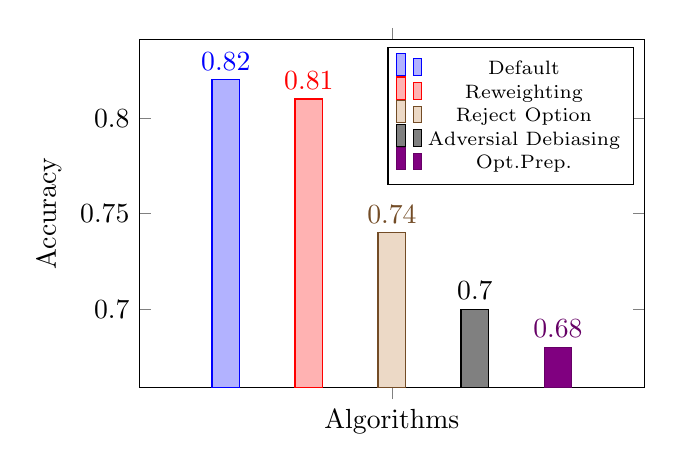
\begin{tikzpicture}
\begin{axis}[
    ybar=20pt,
    enlargelimits=0.15,
    legend style={font=\scriptsize,row sep=-0.1cm},
    ylabel={Accuracy},
    symbolic x coords={Algorithms},
    xtick=data,
    nodes near coords,
    nodes near coords align={vertical},
    ]
\addplot coordinates {(Algorithms,.82)};
\addplot coordinates {(Algorithms,.81)};
\addplot coordinates {(Algorithms,.74)};
\addplot coordinates {(Algorithms,.70)};
\addplot coordinates {(Algorithms,.68)};
\legend{Default,Reweighting,Reject Option,Adversial Debiasing,Opt.Prep.}
\end{axis}
\end{tikzpicture}
\caption{When fairness is detrimental to predictive performance.}\label{fig:Fairness}
\end{wrapfigure}
Our experience is that most of the fairness algorithms, including
adversarial debiasing   achieve fairness by damaging
predictive performance.  \fig{Fairness} shows that various fairness algorithms damage model accuracy to achieve fairness (tested on  Adult Census Income with protected attribute - "Sex")~\cite{IBM}. Note that,
compared to the performance of the default model,
many of the fairness operators results in large decreases in predictive performance.

Later in this proposal, we show that the performance decreases of \fig{Fairness} are optional.
Specifically, we show that if hyperparameter optimizers are asked to manage accuracy {\em and}
fairness, then it is possible to maintain predictive performance while also increase the fairness of the model
Those results are described in the next section.
 
Before going on, we note that there are there are many ways to measure ``fairness'' in a machine learning model.
We using the following definitions:
\bi
\item
 
 A label is called \textit{favorable label} if its  value corresponds to an outcome that gives an advantage to the receiver (e.g. being hired for a job, receiving a loan).
 \item
A \textit{protected attribute} is an attribute that divides a population into two groups that have difference in terms of benefit received  (e.g. race, sex, gender). These attributes are not universal, but are specific to application.
 \item
\textit{Group fairness} is the goal that based on the protected attribute, privileged and unprivileged groups will be treated similarly. 
 \item
\textit{Individual fairness} is the goal of similar individuals will receive similar outcomes.  For
this current proposal, we focus on  Group fairness only.
 \item
{\em Bias} is a systematic error~\cite{bias_systemetic}
and our main concern is unwanted bias that puts privileged groups at a systematic advantage and unprivileged groups at a systematic disadvantage. 
\ei

A \textit{fairness metric} is a quantification of unwanted bias in models or training data~\cite{IBM}. 
For the experiments reported later in this paper, we use two such metrics:
\bi
\item \textbf{Equal Opportunity Difference(EOD)}:    delta of true positive rates in unprivileged \& privileged groups~\cite{IBM}. 
\item \textbf{Average Odds Difference(AOD)}: The average delta in false positive rates and true positive rates between privileged and unprivileged groups~\cite{IBM}.
\ei
A value of 0 implies that both groups have equal benefit, a value lesser than 0 implies higher benefit for the privileged group and a value greater than 0 implies higher benefit for the unprivileged group. In this study, we have taken absolute value of these metrics. 


% \subsection{About Hyperparameter Optimization}\label{tion:hbo}
% The previous section described fairness metrics.
% This section describes automatic methods for altering machine
% learners in order to generate   models that perform well on those metrics. 
  
% Every machine learning algorithm has ``magic'' control parameters. For example:
% \bi
% \item Random forests have a hyperparameter that specifics how many trees in the forest;
% \item 
% When a support vector machines use some kernel and that kernel is specified by a set of parameters, 
% then that kernel and its settings are hyperparameters.
% \item
% When a neural nets use a certain network topology that includes $X$ nodes per layer, then than topology and that value $X$ are hyperparameters. 
% \ei

% \begin{wraptable}{r}{3in}
% \small
% \begin{tabular}{|p{2.9in}|}\hline
% \rowcolor{gray!20}
% If TN, FN, FP, TP are  true negatives, false negatives, false positives,  true positives, then:
% \bi
% \item
% {\em prec} = Precision = TP/(TP+FP) which  measures  the percentage of the predicted class that are actual members of the target class.
% \item 
% {\em pd} = Recall = TP/(TP+FN) which measures the percentage of the actual targets that are predicted to be targets.
% \item
% {\em pf} = False Alarms = FP/(FP+TN), the percentage of the non-target artifacts that are reported as part of the target class;  
% \ei\\\hline
% \end{tabular}
% \caption{Standard   machine learning metrics.}\label{tbl:metrics}
% \end{wraptable} ``Off of the shelf''
%  learners   come
% with   defaults for  control parameters, which may be sub-optimal. For example,
% in the  distance function  $d(x,y,p)=\left(\sum_i (x_i-y_i)^p\right)^{1/p}$,
% a standard default is $p=2$ (i.e. Euclidean distance). Yet Agrawal et al.~\cite{agrawal2017better}  found that
% $p>2$ worked much better for their processing. 



% Hyperparameter optimizers are automatic tools to find better control parameters~\cite{biedenkapp2018hyperparameter}~\cite{franceschi2017forward}. 
% This is done by experimenting with adjustments to the control parameters of a learner. 
% When done using 21st century optimizers (e.g. NSGA-2~\cite{deb00afast}, IBEA~\cite{Zitzler04indicator-basedselection}, MOEA/D~\cite{zhang07}, FLASH~\cite{nair18}), it is now possible to optimizer for multiple goals (even when they are competing). 
%  PI Menzies has had much success  with   
% hyperparameter optimizers  to automatically determine which learner to use, and what settings to apply to those learners~\cite{fu2016tuning,chen2017riot,nair2017flash,agrawal2017better,fu2017revisiting,nair2017using,mathew2017shorter,nair2017faster,chen2017beyond,nair2016accidental,fu2016differential,chen2016sampling,agrawal2016wrong,agrawal2018better}.
% In all that work, the optimizers sought ways to improve standard performance measures
% like recall, precision, and false alarm (defined in \tbl{metrics}).
% In this  proposal, we 
% we will  explore hyperparamter optimizers that seek to manage these standard performance
% measures {\em as well as } the fairness metrics described above.


% There are  many ways to implement hyperparameter optimizers.
% \textit{Grid search}~\cite{bergstra2011algorithms} 
%   creates   
% $C$ nested for-loops to explore   $C$ control parameters.  Bergstra et al. depreciate grid search arguing that (a)~the best hyperparameters are usually found within a very small region of the total space;  and (b)~a grid search that is fine-grained enough to find that region for any learner and any data set would be very slow indeed~\cite{bergstra2011algorithms}

 


% \begin{figure} 
% \small
% \begin{center}
% \begin{tabular}{|r|p{5in}|}
% \hline
%  &\cellcolor{gray!20}
% Start with data $D$ and a small sample $S \subset D$ of, say, 20 examples,
% labelled with their  goals values.
% \\
% LOOP:&Using $S$ and a  data miner, build one model per goal.  In standard BPO, 
% a Gaussian Process Model (GPM) is used for this step. FLASH replaces
% GPM with CART decision trees
% so the resulting systems
% scales to much larger problems; and the learned model is simple and succinct
% enough to show to business users~\cite{nair2017flash}. 
% \\

% &\cellcolor{gray!20}Using those models, guess goal values for  
% $D-S$.
% \\
% &Select   $X \in D-S$ with the ``best''  guesses.  BPO
% collects information only on the next most informative example. In our current favorite
% implementation~\cite{nair2017flash} we use a random project method to find the $X$ that most maximizes
% our goals (across a wide range of possible weighting questions).
% \\ 
% &\cellcolor{gray!20}Evaluate  $X$s' goals. 
% \\
% &
% Let $S=S+X$.  
% \\
 
% &\cellcolor{gray!20} Go to ``LOOP:''
% \\\cline{2-2} \hline
% \end{tabular}
% \end{center}
% \caption{     Hyperparameter optimizer with FLASH~\cite{nair18}.}\label{tbl:flash}
% \end{figure}
 
% ~\textit{Random search}~\cite{bergstra2012random} sets up ranges  of hyperparameter values and select random combinations to train the model and evaluate. 
% There are many such methods including those that use genetic algorithms
% such as  NSGA-2~\cite{deb00afast}, IBEA~\cite{Zitzler04indicator-basedselection}, or MOEA/D~\cite{zhang07}. While an effective strategy, random search may require
% too many evaluations to be practice.

% In contrast to Grid or Random search, \textit{Bayesian optimization}~\cite{pelikan1999boa} keeps track of past evaluation results and use them to build a probabilistic model mapping hyperparameters to a probability of a score on the objective function \cite{Will_Koehrsen}. This probabilistic model is called ``surrogate'' for the objective function. The idea is to find the next set of hyperparameters to evaluate on the actual objective function by selecting hyperparameters that perform best on the surrogate function.

% \textit{Sequential model-based optimization (SMBO)} \cite{hutter2011sequential} is a formalization of Bayesian optimization. It runs trials one by one sequentially, each time trying better hyperparameters using Bayesian reasoning and updating the surrogate model \cite{Will_Koehrsen}. 
% Recently~\cite{nair18}, we have had   success  
% an SMBO algorithm called  FLASH,   The  pseudo code of \tbl{flash}     shows how FLASH  minimizes
%   evaluating different tunings
%   by   collecting information on only the most interesting examples.


% % \textbf{FLASH: A Fast Sequential Model-Based Method:}
% % Nair et al. \cite{8469102} proposed a fast SMBO approach called FLASH for multiobjective optimization. FLASH's acquisition function uses Maximum Mean. Maximum Mean returns the sample (configuration) with the highest expected (performance) measure. FLASH models each objective as a separate performance (CART) model. Because the CART model can be trained for one performance measure or dependent value. Nair reports that FLASH runs orders of magnitude faster than NSGA-II, but that was for software configuration problems. This work is the first study to try using  FLASH to optimize for learner performance while at the same time improving fairness.



% % the worst of which is 
% % a {\em grid search} which creates  try many combinations of $C$ parameters
% % using $C$ nested for-loops~\cite{Bergstra:2012}.
% % Bergstra et al. depreciates grid search arguing that (a)~the best hyperparameters are found
% % within a very small region of the total space; and (b)~a grid search that is fine-grained
% % enough to find that  region for any learner and any dataset would be very slow indeed~\cite{Bergstra:2012}.

% % require thousands to millions of executions of a learner. 

% % Differential evolution is just one in a large suite of possibly useful stochastic optimization algorithms
% % that PI Menzies has used to improve different data mining tasks~\cite{fu2016tuning,chen2017riot,nair2017flash,agrawal2017better,agrawal2017better,fu2017revisiting,nair2017using,mathew2017shorter,nair2017faster,chen2017beyond,nair2016accidental,fu2016differential,chen2016sampling,agrawal2016wrong}.
% % For example 

  
  
% \begin{table}
% \centering
% \footnotesize
% \caption{Optimizing just for fairness.  
% Change in  Recall and False alarm before and after bias mitigation. Gray= improvement; black= damage.
% From~\cite{Chakraborty}.}
% \label{tbl:fairness_cost}
% \begin{tabular}{|l|c|c|r|r|r|r|}\cline{4-7}
 
% \multicolumn{3}{c}{~}
% &\multicolumn{2}{|p{.7in}}{{\em larger} values are {\em better}}&
% \multicolumn{2}{|p{.8in}|}{{\em smaller} values are {\em better}}\\
% \rowcolor[HTML]{C0C0C0} 
% \cellcolor[HTML]{C0C0C0} & 
% \multicolumn{1}{l|}{\cellcolor[HTML]{C0C0C0}} & 
% \multicolumn{1}{l|}{\cellcolor[HTML]{C0C0C0}} & \multicolumn{2}{c|}{\cellcolor[HTML]{C0C0C0}Recall} & \multicolumn{2}{c|}{\cellcolor[HTML]{C0C0C0}False alarm} \\ \cline{4-7} 


% \rowcolor[HTML]{C0C0C0} 
% \multirow{-2}{*}{\cellcolor[HTML]{C0C0C0}Algorithm} & \multicolumn{1}{l|}{\multirow{-2}{*}{\cellcolor[HTML]{C0C0C0}Dataset}} & \multicolumn{1}{l|}{\multirow{-2}{*}{\cellcolor[HTML]{C0C0C0}\begin{tabular}[c]{@{}l@{}}Protected \\ Attribute\end{tabular}}} & \multicolumn{1}{c|}{\cellcolor[HTML]{C0C0C0}Before} & \multicolumn{1}{l|}{\cellcolor[HTML]{C0C0C0}After} & \multicolumn{1}{c|}{\cellcolor[HTML]{C0C0C0}Before} & \multicolumn{1}{l|}{\cellcolor[HTML]{C0C0C0}After} \\ \hline
% \multicolumn{1}{|c|}{} &  & Sex & 83 & \cellcolor[HTML]{FFFFFF}{\color[HTML]{333333} 83} & 34 & \cellcolor[HTML]{333333}{\color[HTML]{FFFFFF} 43} \\ \cline{3-7} 
% \multicolumn{1}{|c|}{} & \multirow{-2}{*}{Adult} & Race & 83 & \cellcolor[HTML]{FFFFFF}{\color[HTML]{333333} 83} & 34 & \cellcolor[HTML]{333333}{\color[HTML]{FFFFFF} 35} \\ \cline{2-7} 
% \multicolumn{1}{|c|}{} &  & Sex & 60 & 60 & \cellcolor[HTML]{FFFFFF}{\color[HTML]{333333} 27} & \cellcolor[HTML]{333333}{\color[HTML]{FFFFFF} 29} \\ \cline{3-7} 
% \multicolumn{1}{|c|}{} & \multirow{-2}{*}{Compas} & Race & 62 & \cellcolor[HTML]{333333}{\color[HTML]{FFFFFF} 61} & \cellcolor[HTML]{FFFFFF}{\color[HTML]{333333} 27} & \cellcolor[HTML]{333333}{\color[HTML]{FFFFFF} 34} \\ \cline{2-7} 
% \multicolumn{1}{|c|}{} &  & Sex & 70 & \cellcolor[HTML]{333333}{\color[HTML]{FFFFFF} 69} & \cellcolor[HTML]{FFFFFF}66 & \cellcolor[HTML]{333333}{\color[HTML]{FFFFFF} 77} \\ \cline{3-7} 
% \multicolumn{1}{|c|}{\multirow{-6}{*}{Reweighing}} & \multirow{-2}{*}{German} & Age & 70 & \cellcolor[HTML]{C0C0C0}71 & \cellcolor[HTML]{FFFFFF}66 & \cellcolor[HTML]{C0C0C0}25 \\ \hline
%  &  & Sex & 83 & \cellcolor[HTML]{333333}{\color[HTML]{FFFFFF} 76} & \cellcolor[HTML]{FFFFFF}34 & \cellcolor[HTML]{333333}{\color[HTML]{FFFFFF} 35} \\ \cline{3-7} 
%  & \multirow{-2}{*}{Adult} & Race & 83 & 83 & \cellcolor[HTML]{FFFFFF}34 & \cellcolor[HTML]{333333}{\color[HTML]{FFFFFF} 37} \\ \cline{2-7} 
%  &  & Sex & 60 & 60 & \cellcolor[HTML]{FFFFFF}27 & \cellcolor[HTML]{333333}{\color[HTML]{FFFFFF} 29} \\ \cline{3-7} 
%  & \multirow{-2}{*}{Compas} & Race & 62 & \cellcolor[HTML]{C0C0C0}{\color[HTML]{333333} 65} & \cellcolor[HTML]{FFFFFF}27 & \cellcolor[HTML]{333333}{\color[HTML]{FFFFFF} 29} \\ \cline{2-7} 
%  &  & Sex & 70 & \cellcolor[HTML]{333333}{\color[HTML]{FFFFFF} 69} & \cellcolor[HTML]{FFFFFF}66 & \cellcolor[HTML]{C0C0C0}{\color[HTML]{333333} 36} \\ \cline{3-7} 
% \multirow{-6}{*}{\begin{tabular}[c]{@{}l@{}}Optimized \\ Pre-\\ processing\end{tabular}} & \multirow{-2}{*}{German} & Age & 70 & \cellcolor[HTML]{333333}{\color[HTML]{FFFFFF} 68} & \cellcolor[HTML]{FFFFFF}66 & \cellcolor[HTML]{C0C0C0}{\color[HTML]{333333} 58} \\ \hline
%  &  & Sex & 82 & \cellcolor[HTML]{C0C0C0}83 & 35 & \cellcolor[HTML]{333333}{\color[HTML]{FFFFFF} 42} \\ \cline{3-7} 
%  & \multirow{-2}{*}{Adult} & Race & 82 & 82 & 35 & 35 \\ \cline{2-7} 
%  &  & Sex & 60 & 60 & 27 & \cellcolor[HTML]{333333}{\color[HTML]{FFFFFF} 28} \\ \cline{3-7} 
%  & \multirow{-2}{*}{Compas} & Race & 60 & 60 & 27 & \cellcolor[HTML]{333333}{\color[HTML]{FFFFFF} 28} \\ \cline{2-7} 
%  &  & Sex & 70 & \cellcolor[HTML]{C0C0C0}75 & 66 & \cellcolor[HTML]{C0C0C0}61 \\ \cline{3-7} 
% \multirow{-6}{*}{\begin{tabular}[c]{@{}l@{}}Adversial\\ Debiasing\end{tabular}} & \multirow{-2}{*}{German} & Age & 70 & \cellcolor[HTML]{333333}{\color[HTML]{FFFFFF} 69} & 50 & \cellcolor[HTML]{333333}{\color[HTML]{FFFFFF} 72} \\ \hline
%  &  & Sex & 83 & \cellcolor[HTML]{333333}{\color[HTML]{FFFFFF} 24} & 34 & \cellcolor[HTML]{C0C0C0}05 \\ \cline{3-7} 
%  & \multirow{-2}{*}{Adult} & Race & 83 & \cellcolor[HTML]{333333}{\color[HTML]{FFFFFF} 28} & 34 & \cellcolor[HTML]{C0C0C0}04 \\ \cline{2-7} 
%  &  & Sex & 62 & \cellcolor[HTML]{C0C0C0}{\color[HTML]{333333} 97} & 27 & \cellcolor[HTML]{333333}{\color[HTML]{FFFFFF} 89} \\ \cline{3-7} 
%  & \multirow{-2}{*}{Compas} & Race & 62 & \cellcolor[HTML]{C0C0C0}{\color[HTML]{333333} 68} & 27 & \cellcolor[HTML]{333333}{\color[HTML]{FFFFFF} 38} \\ \cline{2-7} 
%  &  & Sex & 70 & \cellcolor[HTML]{C0C0C0}{\color[HTML]{333333} 96} & 66 & \cellcolor[HTML]{333333}{\color[HTML]{FFFFFF} 95} \\ \cline{3-7} 
% \multirow{-6}{*}{\begin{tabular}[c]{@{}l@{}}Reject\\ Option\end{tabular}} & \multirow{-2}{*}{German} & Age & 70 & 70 & 66 & 66 \\ \hline
%  &  & Sex & 83 & \cellcolor[HTML]{333333}{\color[HTML]{FFFFFF} 78} & 39 & \cellcolor[HTML]{333333}{\color[HTML]{FFFFFF} 40} \\ \cline{3-7} 
%  & \multirow{-2}{*}{Adult} & Race & 83 & \cellcolor[HTML]{333333}{\color[HTML]{FFFFFF} 78} & 39 & \cellcolor[HTML]{C0C0C0}35 \\ \cline{2-7} 
%  &  & Sex & 65 & \cellcolor[HTML]{333333}{\color[HTML]{FFFFFF} 63} & 38 & \cellcolor[HTML]{333333}{\color[HTML]{FFFFFF} 40} \\ \cline{3-7} 
%  & \multirow{-2}{*}{Compas} & Race & 65 & 65 & 38 & \cellcolor[HTML]{333333}{\color[HTML]{FFFFFF} 39} \\ \cline{2-7} 
%  &  & Sex & 74 & \cellcolor[HTML]{333333}{\color[HTML]{FFFFFF} 72} & 20 & \cellcolor[HTML]{333333}{\color[HTML]{FFFFFF} 33} \\ \cline{3-7} 
% \multirow{-6}{*}{\begin{tabular}[c]{@{}l@{}}FLASH\\ optimizes for\\ AOD \& EOD\end{tabular}} & \multirow{-2}{*}{German} & Age & 74 & \cellcolor[HTML]{333333}{\color[HTML]{FFFFFF} 68} & 20 & \cellcolor[HTML]{333333}{\color[HTML]{FFFFFF} 45} \\ \hline
% \end{tabular}
% \end{table}
 

\section{Preliminary Results}\label{preliminary}


Recent studies have shown that hyperparameter optimization can achieve better performance than using ``off-the-shelf'' configurations in several research areas in software engineering, e.g., software effort estimation\cite{xia2018hyperparameter} and software defect prediction\cite{osman2017hyperparameter}. We are first to apply hyperparameter optimization in software fairness domain~\cite{Chakraborty}.

%  \subsection{  Hyperparameter Optimization \& Fairness}\label{tion:ms}
% \tbl{fairness_cost} show what happens when the above seven steps
% of FLASH 
% are applied to fairness.
% \tbl{fairness_cost} applies various fairness operators (taken from   github.com/IBM/AIF360) to protect various attributes
% within the Adult, Compas, and German data sets (these are standard data sets used for experimentation in this field).


% In \tbl{fairness_cost}, gray denotes an improvement in predictive
% performance and black denotes worse predictive performance. 
% The last few lines  of     \tbl{fairness_cost}  shows FLASH optimizing in order to minimize
% the absolute value of both EOD {\em and} AOD (the fairness metrics described in the last section).
% In those results, we asked FLASH to minimize the
% absolute value of EOF and AOD. To do this,
% we let FLASH tune four hyperparameters for two learners:
% \bi
% \item Logistic regression (which learns an equation):
% \bi
% \item C: Inverse of regularization strength where smaller values specify stronger regularization.
% \item
% penalty: Used to specify the norm used in the penalization applied to the model.
% \item solver: Algorithm to use in the optimization problem
% \item maxiter: Maximum number of iterations taken for the solvers to converge.
% \ei
% \item
% CART (which learns an decision tree):
% \bi
% \item criterion: The function to measure the quality of a split.
% \item splitter: The strategy used to choose the split at each node.
% \item minsamplesleaf: The minimum number of samples required to be at a leaf node. A split point at any depth will only be considered if it leaves at least certain number of training samples in each of the left and right branches.
% \item minsamplessplit: The minimum number of samples required to split an internal node.
% \ei
% \ei
% In the FLASH results, 
% the two things to observe from
% \tbl{fairness_cost}  are:
% \bi
% \item
% Firstly,
% there are many  black entries; i.e.
% applying the fairness operators has negative impact on predictive performance.
% Some of the changes in  in performance are negligible (e.g. false alarms changing from 27 to 28).
% But in other cases, the impact of applying the fairness operators is truly alarming, particularly for the false alarm rates (e.g  for ``reject option'', we can see false alarms increasing from 27\% to 89\% in some cases).

% This negative impact of fairness operators on performance prowess is somewhat alarming. Historically,
% it was the original motivator for this research.
% \item
% Secondly, 
% of all the fairness operators, FLASH has the most black entries
% in both recall and false alarm.  
% It is easy to explain, and to fix, FLASH's poor performance in   \tbl{fairness_cost}.
% Hyperparameter optimizers are servants that follow our instructions. In  \tbl{fairness_cost}, we told to
% FLASH to optimize for fairness, but not to care about recall and false alarms. Not surprisingly, this lead
% to FLASH generating models with  poor predictive prowess.
% \ei


% \begin{table}[!t]
% \centering
% \footnotesize
% \caption{Optimizing for fairness, lower false alarm and higher recall. Gray=improvement; black=damage.
% Note that, compared to Table~\ref{tbl:fairness_cost}, there is far less damage. From~\cite{Chakraborty}.}
% \label{tbl:multiobjective_results}
% \begin{tabular}{|l|l|c|r|r|r|r|r|r|>{\columncolor[HTML]{FFFFFF}}r |r|}
% \cline{4-11}
 
% \multicolumn{3}{c}{~}
% &\multicolumn{2}{|p{.7in}}{{\em larger} values are {\em better}}&
% \multicolumn{2}{|p{.8in}|}{{\em smaller} values are {\em better}}&
% \multicolumn{4}{c|}{{\em smaller} values are {\em better}} \\

% \hline
% \cellcolor[HTML]{C0C0C0} & \cellcolor[HTML]{C0C0C0} & \multicolumn{1}{l|}{\cellcolor[HTML]{C0C0C0}} & \multicolumn{2}{c|}{\cellcolor[HTML]{C0C0C0}Recall} & \multicolumn{2}{c|}{\cellcolor[HTML]{C0C0C0}\begin{tabular}[c]{@{}c@{}}False \\ alarm\end{tabular}} & \multicolumn{2}{c|}{\cellcolor[HTML]{C0C0C0}AOD} & \multicolumn{2}{c|}{\cellcolor[HTML]{C0C0C0}EOD} \\ \cline{4-11} 
% \multirow{-2}{*}{\cellcolor[HTML]{C0C0C0}Model} & \multirow{-2}{*}{\cellcolor[HTML]{C0C0C0}Dataset} & \multicolumn{1}{l|}{\multirow{-2}{*}{\cellcolor[HTML]{C0C0C0}\begin{tabular}[c]{@{}l@{}}Protected \\ Attribute\end{tabular}}} & \multicolumn{1}{c|}{\cellcolor[HTML]{C0C0C0}Before} & \cellcolor[HTML]{C0C0C0}After & \multicolumn{1}{c|}{\cellcolor[HTML]{C0C0C0}Before} & \cellcolor[HTML]{C0C0C0}After & \multicolumn{1}{c|}{\cellcolor[HTML]{C0C0C0}Before} & \cellcolor[HTML]{C0C0C0}After & \multicolumn{1}{c|}{\cellcolor[HTML]{C0C0C0}Before} & \cellcolor[HTML]{C0C0C0}After \\ \hline
% \multicolumn{1}{|c|}{} &  & Sex & 83 & \cellcolor[HTML]{333333}{\color[HTML]{FFFFFF} 78} & 39 & \cellcolor[HTML]{C0C0C0}{\color[HTML]{333333} 32} & 31 & \cellcolor[HTML]{C0C0C0}09 & 49 & \cellcolor[HTML]{C0C0C0}15 \\ \cline{3-11} 
% \multicolumn{1}{|c|}{} & \multirow{-2}{*}{Adult} & Race & 83 & \cellcolor[HTML]{333333}{\color[HTML]{FFFFFF} 80} & 39 & \cellcolor[HTML]{C0C0C0}{\color[HTML]{333333} 31} & 14 & \cellcolor[HTML]{C0C0C0}04 & 22 & \cellcolor[HTML]{C0C0C0}08 \\ \cline{2-11} 
% \multicolumn{1}{|c|}{} &  & Sex & 65 & 65 & \cellcolor[HTML]{FFFFFF}{\color[HTML]{333333} 38} & 38 & 24 & 24 & 29 & 29 \\ \cline{3-11} 
% \multicolumn{1}{|c|}{} & \multirow{-2}{*}{Compas} & Race & 65 & 65 & \cellcolor[HTML]{FFFFFF}{\color[HTML]{333333} 38} & 38 & 12 & 12 & 16 & 16 \\ \cline{2-11} 
% \multicolumn{1}{|c|}{} &  & Sex & 74 & 74 & \cellcolor[HTML]{FFFFFF}2 & 2 & 12 & 12 & 04 & 04 \\ \cline{3-11} 
% \multicolumn{1}{|c|}{\multirow{-6}{*}{\begin{tabular}[c]{@{}c@{}}Logistic\\ regression\end{tabular}}} & \multirow{-2}{*}{German} & Age & 74 & 74 & \cellcolor[HTML]{FFFFFF}2 & 2 & 44 & 44 & 08 & 08 \\ \hline
%  &  & Sex & 83 & 83 & \cellcolor[HTML]{FFFFFF}36 & 36 & \cellcolor[HTML]{FFFFFF}29 & 29 & 46 & 46 \\ \cline{3-11} 
%  & \multirow{-2}{*}{Adult} & Race & 83 & 83 & \cellcolor[HTML]{FFFFFF}36 & 36 & \cellcolor[HTML]{FFFFFF}14 & 14 & 24 & 24 \\ \cline{2-11} 
%  &  & Sex & 65 & 65 & \cellcolor[HTML]{FFFFFF}35 & 35 & \cellcolor[HTML]{FFFFFF}25 & 25 & 29 & 29 \\ \cline{3-11} 
%  & \multirow{-2}{*}{Compas} & Race & 65 & 65 & \cellcolor[HTML]{FFFFFF}35 & 35 & \cellcolor[HTML]{FFFFFF}23 & 23 & 26 & 26 \\ \cline{2-11} 
%  &  & Sex & 74 & 74 & \cellcolor[HTML]{FFFFFF}5 & \cellcolor[HTML]{333333}{\color[HTML]{FFFFFF} 29} & \cellcolor[HTML]{FFFFFF}15 & \cellcolor[HTML]{C0C0C0}1 & 14 & \cellcolor[HTML]{C0C0C0}3 \\ \cline{3-11} 
% \multirow{-6}{*}{CART} & \multirow{-2}{*}{German} & Age & 74 & 74 & \cellcolor[HTML]{FFFFFF}5 & \cellcolor[HTML]{333333}{\color[HTML]{FFFFFF} 29} & \cellcolor[HTML]{FFFFFF}60 & \cellcolor[HTML]{C0C0C0}53 & 21 & \cellcolor[HTML]{C0C0C0}7 \\ \hline
% \end{tabular}
% \end{table}

% \subsection{  Four Goal Optimization}\label{tion:ms}
% To fix FLASH, all we need to do is ask it to optimize for four goals: improve EOD {\em and} improve AOD {\em and} minimize
% false alarms {\em and} maximize recall. The results of this four goal optimization run is shown in
% \tbl{multiobjective_results}. Note that, in these results,
% there are far fewer  black cells \tbl{multiobjective_results} than in  \tbl{fairness_cost}; i.e. 
% if   our optimizer know
% all the goals that matter, then it can generate better solutions across those spaces of goals.
% Also, 
% unlike \fig{Fairness}, we see that with 4-goal hyperparameter optimization, fairness need not be detrimental
% to   predictive performance since, 
% as seen in \tbl{multiobjective_results}:
% \bi
% \item
% Using logistic regression, in the Adult data set, we can improve AOD and EOD for sex and race by almost three
% times.
% \item Even larger improvements are available, perhaps using other learners.
% For example, using CART, in the German data set, for the sex attributes,   EOD and AOD are improved five to fifteen times.
% \ei
% Improving fairness might require switching the learning algorithm. As evidence of that,
% note that:
% \bi
% \item
% Logistic regression   improves
% fairness in the Adult data set, not mot for German.
% \item
% For that data set, to improve fairness, we need to use CART.
% \ei
% This last finding is particularly troubling for Model Stores. Usually, the models in Model Stores are hardwired
% to a specific learner
% but \tbl{multiobjective_results} indicates that maintaining fairness can requre exploring a wider range of  options. 

 


\section{Open Issues}\label{open}

 
% The goal of this proposal is to   make hyperparameter optimization for fairness so fast and effective
% that it can routinely be applied to model generation (via data miners).

\noindent
The above results are promising, but incomplete, for several reasons:
\bi
\item
The above results only assess the success
of optimizing-for-fairness via fairness measures (EOD and AOD) and predictive prowess (recall
and false alarm). Another important assessment criteria is the 
{\em time} and associated  {\em CPU cost} of generating those models. 
Even our most optimized optimizer (FLASH) needs to execute learners 20 to 100 times.
That is, when exploring just one learner, hyperparameter optimization can take two
orders of magnitude more CPU to reach its conclusions.
This an important point since,
as stated in the introduction, 
any method requiring excessive addition CPU is contraindicated for Model Store models.
Within a Model Store, users pay for access to the machine learner
as well as the CPU required to run, test, and possibly tune, that model.
That is, the users
purchasing those models must foot the bill for the associated CPU costs.
If Model Store clients have a choice of models, and some are orders of magnitude cheaper to buy than others
(i.e. the ones that do not use hyperparameter optimization), then the natural tendency of consumers
will be to favor the cheaper product (even if that cheaper product is more unfair).
\item
The  above results make no use of any prior experience with 
applying   optimization-for-fairness to a learner. This is a major deficiency in our prior work since,
in the context of Model Stores, similar models would be generated many times (whenever multiple
users hired and applied the same Model Store app). In theory, prior optimization
experience might be used to speed-up any subsequent optimization study.  
\item
The above results are based on only a few data sets--
so we need to explore models.
Of particular importance here is the
last result mentioned above; i.e. that sometimes the best hyperparameter optimization
is achieved via switching learners.  Theoretically, if we studied enough data sets and enough learners, we might find that some small set of learners are always
generating the best optimize-for-fairness results. If this were true then this would significantly reduce to the computational cost of hyperparameter optimization for fairness (since any optimize-for-fairness study would have to try  fewer   learners). 
\item
The above results
are based on binary classifiers with simplistic measures for predictive prowess
(just the measures of \tbl{metrics}). There are many more measures we have yet to explore. For example, consider the {\em Hospital  Readmission} model described on \tion{problem}. 
For that model, predictive prowess means minimizing the time/cost of hospitalization
while also minimizing the probability of negative medical outcomes (a.k.a. death).  
\item
In terms of \tbl{multicol}, the above results just explore one kind of fairness operator;
specifically the  ``in-processing'' kind of fairness operator that adjusts the learning process.
There are other kinds of fairness operators that need to be explored such as pre- and post- processing operators. 
\item
Section~\tion{ms} mentions about the hyperparameter options explored as part of using optimizer but the hyperparameter optimization space of these algorithms are much more vast. Exploring these options will require vast amount of CPU resources. Thus we will require to make a trade-off between exploring the extend of hyperparameter space and cost awareness of the models.
\item
Quality of data used in training can impact the predictive power of model in multiple ways which is why data preprocessing is a major area of research. There are various techniques that can be applied and utilized to improve predictive results such as removals of outliers, data balancing by minority oversampling or majority down sampling, attribute section, data weighting etc. All these different techniques need to be explored to achieve desired performance. 

\ei

\newcommand{\head}[1]{\noindent{\bf \underline{#1}}:}

\section{Research Plan}\label{tion:plan}


\noindent
To address these open issues, our research plan  has five parts:
\be
\item
{\bf Initial Set-up}:
In steps
one,two,three and four, we conduct some background studies
to collect the data needed to assess the results of steps five and beyond.
\item
{\bf (re)Building {\IT}}:
Next, in steps five to eight, we explore  the three kinds
of fairness operators described in \tbl{multicol}; i.e. pre-, in- and post- processing of machine learners. The tool we call {\IT} is a combination
of these three operators, plus a set of heuristics telling us
when to use which operator.
\item
{\bf Extend to Multiple Learners:}
Initially, for steps one to eight, 
we will assume that the machine learner is not
to be changed (so we will use whatever learner appears is found in  the Model Store
application). But after that, we will loop back though steps one to eight
allowing the optimizer-for-fairness to switch learners if it wants
to. By doing this, we will (a)~get some
quick initial results; then
(b)~be able to assess the value of optimize-for-fairness using
single vs multiple learners.
\ei
Finally, running in parallel across the other parts, we have two other important activities:
\begin{enumerate} 
\item
{\bf Packaging and Sharing of Methods:}
Whenever we have evidence that we can significantly reduce
the CPU cost of optimization-as-fairness, we will (a)~package up our software as a public domain Python package; (b)~reach out to Model Store managers and app store developers to share our results with them.
\item
{\bf Comparisons with other Fairness Research}: Fairness research is a very active research area. 
Hence, we foresee that over the course of this grant, many  fairness operators will be published.
Accordingly, it is important that what results obtained in this grant are compared with the state-of-the-art
in the fairness literature. 
\end{enumerate}
For details notes on all these five parts, see below.

 \subsection{Part1: Initial Set-up}
 
\subsubsection{Step 1. Build ``Lab Rats''}\label{tion:labrat}
In this step, we will build our  ``lab rats''; i.e. models that will be explored using optimization-for-fairness.
In this first step, we will  repeat the analysis 
of \tion{problem}, but at a much larger scale; i.e. for the hundreds of known models
in the Model Stores. 
We would then study those models in order to generate
a catalogue of   (a)~the available models;  (b)~lists of developers (for the Model Store apps) and~(c)~lists of data/learners used; (d)~list attributes within each model that we wish to protect (e.g. age, race, gender, income, etc). 
Using this list we would 
\bi
\item Extend our definitions of predictive prowess beyond the list of \tbl{metrics}.
For example, to repeat the example
offered above,
the  {\em Hospital  Readmission} model described in \tion{problem}
might need to minimize
the time/cost of hospitalization
while also minimizing the probability of negative medical outcomes.
Other models may have other definitions of ``good'' predictions: e.g. safety-critical
apps may allow large false negative results, just as long as the recall results
are exception.
\item
Contact the Model Store app developers, informing them of
our research and asking them to contribute data and models. There are many ways we could contact them,
the easiest being to leave remarks in the comments sections of the Model Store.
We would negotiate with them
a non-disclosure agreement with the following clause.
If we find fairness issues in their models, they will be the first to be told.
After that, that result will be embargoed for 12 months such that no outside
is aware of fairness issues in that model for one year after we notify the Model
Store app developers.
\item
Look for models that we can recreate, within our own lab, using public domain
data and public domain learners. Our preliminary analysis of the Model Stores
suggests that there are numerous such models.
\ei
Just to speak to the practicality of the last point,
we note that  a new trend within  Model Stores
is to include sample data with the Model Store app  (e.g. in the AWS marketplace,
see 
{\em  Attribution prediction, Medical no show prediction, Credit default prediction})
 
 
 \newenvironment{success}[1]{ 
 \vspace{-1mm}
 \centerline\noindent\begin{minipage}{.9\linewidth}
    \begin{center}
    \arrayrulecolor{black}
    \begin{tabular}{|p{0.95\linewidth}|}\hline
         \rowcolor{gray!20}
         {\bf Success criteria for ``#1''}}{
    \\\hline\end{tabular}\end{center}\end{minipage}\vspace{1mm}}
    
     
    
\begin{success}{Lab rats}
We know the range of models/learners/evaluation criteria
that exist in the current model stores. Further, we can access
for ourselves a sample of models/learners across that range.
\end{success}

 
\subsubsection{Step 2. Create baselines1 (no tuning)} Here, we will build models using off-the shelf defaults from the learners. 
Currently, we have ready access
to many   machine learning algorithms (see  www.kdnuggets.com/software/libraries.html) including the WEKA JAVA toolkit
and the Scikit-learn Python toolkit. All these learners expose their control parameters.
In this step we will build models using the default parameters then record the observed fairness levels (using EOD and AOD) and predictive prowess
(using success measures appropriate to different models: recall and false alarm where appropriate, and perhaps other measures for other models-- see point4 in the previous section).  


\begin{success}{Baselines1}
We can   execute
for ourselves, outside the Model Stores, many of the
  models available within the Model Stores. 
\end{success}

\subsubsection{Step 3. Create baselines2 (with tuning)} Applying
our standard methods; i.e.
we would conduct optimization-as-fairness
with a machine learning algorithm.  Initially, we will 
conduct those tunings using the FLASH~\cite{nair2017flash} sequential model-based
optimizer described in  \tbl{flash}. Note that while this
optimizer is one the current state-of-the-art algorithms in this field,
as mentioned above, it still requires 20 to 100 executions
of the data miner to achieve its optimization goals. Hence,
in later steps of this proposal, we will strive to reduce the
computational cost of running some new optimization-as-fairness
run via reusing the experience gained in older 
optimization-as-fairness
runs.


\begin{success}{Baseline2}
By comparing with Baseline1,
we can determine how much we can improve fairness without damaging predictive prowess using standard optimizers. Here ``improvement'' will be measured
via fairness measures like EOD and AOD and predictive prowess will be measured
using the performance measures found in Step1.
\end{success}


\subsubsection{Step 4. Cost awareness}\label{tion:costaware} Once the prior step is completed,
we will know the computational cost of optimization-as-fairness.
Using the cost models for the Model Stores, we can then determine the cost to the user of optimization-as-fairness. Using qualitative methods (surveys,
focused interviews), we will learn the   sensitivity of Model
Store users to the these costs. Note that to conduct these qualitative surveys, we will start by  posting  comments   of the review sections on
the   Model Stores. 

This research team has much prior experience with running such qualitative studies~\cite{Menzies:2013:DSS:2486788.2487048,Menzies:2015:ASA:2819009.2819229,Menzies:2016:ADS:2889160.2891047}.


\begin{success}{Cost awareness}
We can draw cost awareness curves showing how much additional
cost-to-use a model impacts the number of purchases of that model.
\end{success}

Once such curves are available, we can define the overall success criteria of this project. In our introduction we said that one of our goals was to apply optimization-for-fairness at    ``not much'' more CPU cost that   than learning without tuning.
By studying the ``knee'' in the cost awareness curves, we can define what
value we need to assign to ``not much''.


 \subsection{Part2: (re)Building {\IT}}
 We will loop through this section many times. Initially
 we will build version1 of {\IT}. Subsequently,
 we will revisit that code and rebuild it (to make a better
 version).

\subsubsection{Step 5. Pre-processing: ``Match''ing Old Tunings} %\label{tion:plan}

 In this step we will
explore pre-processing using   {\bf Match}; i.e.   given $T$ prior tunings and  new data,  run the tuning $T_i$  see in similar prior data.
This approach assumes such prior tunings exists which, in the case
of Model Stores, is quite possible\footnote{When many users
rent and tune the same Model Store app, then the results of 
those tunings will be known to the Model Store app. If these tunings
are cached, then
they could be reused to simplify future tunings.}.
{\bf Match} is common industrial practice~\cite{dlreuse}, particularly
in the deep learning community where training is so lengthy and 
expensive. The black art in {\bf Match} is to select which prior
tuning is best for a new data set. Recently,   Truede and Wagner   added
  some clarity to the black art
  processing of matching to prior tunings~\cite{treude2018per}. They extracted featured from different data sets and used a decision tree learner to predict which prior tuning set
was best for new data:
The obvious advantage of this approach is ``zero cost tuning''; i.e. 
useful tunings can be discovered with no new experimentation. But the
 obvious disadvantages of this approach are:
\bi
\item {\em Closest, but not close enough:} ``Match'' can find the nearest
tuning from the space of old tunings, which is not necessarily
the same thing as the ``best'' tuning. 

\item {\em Negative transfer:} Pan et al.~\cite{Pan2010A}
warn that reusing old knowledge becomes
a problem when old information is no longer relevant for new contexts.
Hence, ``Match'' cannot be recommended unless it also comes with a 
``DontMatch'' operator that warns when reusing old tunings is inappropriate.
Our preliminary results suggest that {\bf DontMatch} might be
built via a meta-analysis of the trees build in the Truede and Wagner 
process (specifically,  look for properties of tree branches that predict for
ineffective transfer).  Note that when {\bf DontMatch} ' reports that 
reusing old tunings is inappropriate, then something else is required
to address the computational cost of optimization-as-fairness
(hence, the next two steps in our research plan).
\item {\em Prior tunings must exist:} Even if the above two points are
not an issue, {\bf Match}  assumes that there exists
old tunings  
for some machine learning method.
Generating those prior tunings incurs a computational cost.
Hence, we will need the CPU reduction methods described in the rest of this proposal.
\ei
To address the above concerns, our research will explore {\bf Match} 
over many models. 

\begin{success}{Match}
 We can operationalize
{\bf Match}  and {\bf DontMatch} .
We can say  just how much
is lost, if anything,  by just using {\bf Match}   compared against  Baseline2 (see above:
running optimization-for-fairness from scratch).  
\end{success}


\subsubsection{Step 6. In-processing with ``Transfer''}
In this step, we  use the results from
{\bf Match}  to guide new optimization-as-fairness studies. 
There are many ways this {\bf Transfer}  can be accomplished
(and the research in this step will determine which works best):
\bi
\item
The space of known old tunings might be used as a probability
distribution to guide mutations for new tunings;
\item
The best old tuning (from {\bf Match}) might be used to initialize 
the internal data structures of our sequential model-based optimizer.  
\item
Some combination of the last two points where 
 our sequential model-based optimizer is initialized using
 items computed by somehow combining prior tunings.
\ei

\begin{success}{Transfer}
We can say  just how much
is gained (if anything at all),
by adding in-processing {\bf Transfer} to the initial
{\bf Match} process.  
\end{success}

\subsubsection{Step 7. Post-processing with ``Patch''}
Once there is much experience with running these models, there will also be much experience
with managing their characteristics errors.
For example, suppose a human
operator realizes that a particular model works worst for (say) non-Caucasian data. That operator might
implement their own {\bf Patch} rule that overwrites a conclusion, in certain contexts.  

Manually learning and maintaining such {\bf Patch}  rules can be a time-consuming and error-prone task.
To handle this kind of problem, PI Menzies has explored incremental
active learning tools\cite{Yu2018,Yu20} that help humans read a large number of examples. These active learners
incrementally learn a model about a human finds interesting or dull. That model can be used to
``rush ahead'' and find fetch examples that are most interesting to humans\footnote{Given
the support vectors of an SVM, the examples that are least/most uncertain and which 
lest/most need to be reviewed
by humans are those that fall far away/within the support vectors.}. 
With this automatic assistant,  humans spend less
time reviewing dull examples. Typically these tools let humans avoid reviewing 80\% or more of the corpus~\cite{Yu2018,Yu20}.

We conjecture that these active learners could be used as a way to record the human experience
of running these models, finding biases, and adjusting the conclusions. That ism
we could use these active learners to implement {\bf Patch} .

\begin{success}{Patch}
We understand the cost and benefits of {\bf Patch} . Note that {\bf Patch}  would be a failure
if it costs excessive human effort to commission or   {\bf Patch}   
only results in negligible improvements to fairness.
\end{success}

\subsubsection{ Step 8. Mix and Match}
We conjecture that none of the above methods, used in isolation, will result in fairer
models with less CPU cost. Rather, we suspect that best results will come from mix-and-matching
the above methods. For example:
\bi
\item Usually, use {\bf Match} 
\item But when {\bf DontMatch} triggers, use the {\bf Transfer} methods to quicker implement 
optimization-as-fairness.
\item Sometimes, replace all the above with some {\bf Patch}ing
\ei
This step will test this conjecture to learn how best to mix-and-match.

\begin{success}{Mix-and-Match}
We understand (a)~the relative cost of benefits of {\bf Match}, {\bf Transfer}  and {\bf Patch} ;
and (b)~when to jump from one method to another.
\end{success}
 
 \subsection{Part3: Extend to Multiple Learners}
 
\subsubsection{ Step 9. Multiple Learners}
Repeat steps steps three to eight, but this time allow optimization-for-fairness to 
try different learners. Note that this will add significant CPU time to optimize-for-fairness.
Hence, we delay working on multiple learners until we've built up an experience base using
single learners.
 

\begin{success}{Multiple Learners}
We understand the cost and benefits of single-vs-multiple learners for
optimization-as-fairness. 
 Note that we would deprecate the use of multiple learners for optimize-for-fairness
 if the additional computational cost of using multiple learners is not justifiable
 via a suitably large improvement in fairness.  
\end{success}

\subsection{Part4: Packaging and Sharing of Methods:}
 
\subsubsection{ Step 10. Dissemination of Results}\label{tion:package}

Finally, running in parallel across the other step,
whenever we have evidence that we can significantly reduce
the CPU cost of optimization-as-fairness, we will (a)~package up our software as a public domain Python package (free to download, install, use); (b)~reach out to Model Store managers and app store developers to share our results with them.
For further details on this point, see the {\em Collaboration Plan} attached
to this proposal.

\subsection{Part5: Comparisons with other Fairness Research} 
\subsubsection{ Step 11. Compare with Related Work}\label{tion:package}

We foresee that over the course of this grant, many fairness operators will be published.  Accordingly, it is important that what results obtained in this grant are compared with the state-of-the-art in the fairness literature.
For this research step, we will maintain a watching brief over publications
in this field and whenever we publish papers/ blog posts on this work,
we will include comparisons against the current state-of-the-art from other
researchers.

 
 \newpage
 
 
For this part
\ei
All the technology discussed above will eb use
There is some work in this area in the AI literature and 

Recent results in the AI literature argue


In 2020, there is much project data readily available on Github. The standard advice is that researchers should ignore most of it.
Kalliamvakou et al. warns that  many repositories on GitHub are not suitable

'
the a
 In their work, they found that when standard text miners cluster documents, those clusters can be dramatically altered merely by changing the input ordering of the training data (i.e. those text clustering algorithms
 exhibited conclusion instability).
 
 These papers are worth revisiting since it is widely cited\footnote{232 and 179 citations respectively in Google Scholar, as of Sept 28, 2020.} and it addresses an important issue. Herbsleb argues convincingly that how groups organize themselves
can be highly beneficial/detrimental to the process of writing code~\cite{Herbsleb14}. Hence, process factors
can be highly informative about what parts of a codebase are buggy. In support
of the Herbsleb hypothesis, prior studies have shown that, for the purpose of defect prediction,
process metrics significantly out-perform product metrics~\cite{Lumpe12,Ra13,bird2009does}. 
Also, if we wish to learn general principles for software engineering that hold across multiple projects, it is better to use process metrics since:
\bi
\item
Process metrics, are much simpler to collect and can be applied in a uniform manner to software written in different languages.  
\item
Product metrics, on the other hand,  can be much harder to collect.
For example, some  static code analysis requires expensive licenses which need updating every time a new version of a language is released~\cite{Devanbu14}.
Also, the collected value for these metrics may not translate between projects since those ranges can be highly specific.
Lastly,
product metrics are far more verbose and hence harder to collect. For example, 
for 722,471 commits studied in this paper, 
data collected required 500 days of CPU (using five machines, 16 cores, 7days). Our process metrics, on the other hand,
were an order of magnitude faster to collect.


for software engienering. ellwethers are a cross-project  learning method. where each

Recently we have been experimenting with ``process metrics''.
Also, if we wish to learn general principles for software engineering that hold across multiple projects, it is better to use process metrics since:
 
Process metrics, are much simpler to collect and can be applied in a uniform manner to software written in different languages.  
 
Product metrics, on the other hand,  can be much harder to collect.
For example, some  static code analysis requires expensive licenses which need updating every time a new version of a language is released~\cite{Devanbu14}.
Also, the collected value for these metrics may not translate between projects since those ranges can be highly specific.
 
 

small sdata differente can lead to differenrt models.

XXX see the same instability when reasoning across similar projects like Zephyr. , If we ask a elarning to generate accurate predictions for data, then it will dilogenyl 

Enter stability-oriented learning. 

For several reasons, we believe it is now possible to learn general conclusions from a diverse space of projects like Figure~\ref{fig:apache} (and the goal of this project is to check those beliefs).
 
Recently we have been experimenting with ``process metrics''.
Also, if we wish to learn general principles for software engineering that hold across multiple projects, it is better to use process metrics since:
 
Process metrics, are much simpler to collect and can be applied in a uniform manner to software written in different languages.  
 
Product metrics, on the other hand,  can be much harder to collect.
For example, some  static code analysis requires expensive licenses which need updating every time a new version of a language is released~\cite{Devanbu14}.
Also, the collected value for these metrics may not translate between projects since those ranges can be highly specific.
 
 
  \subsubsection{Sampling Bias}

\subsection{Evaluation Bias}
We follow their advice and apply a related criteria (with GitHub GraphQL API) for finding useful URLs of related projects (see Table~\ref{tbl:select}).
After that, to remove repositories with irrelevant topics such as ``books'', ``class projects'' or ``tutorial docs'', etc., we create a dictionary of ``suspicious words of irrelevancy'', and remove URLs which contain words in that dictionary (see  Table~\ref{tbl:dict}). After applying the criteria of Table~\ref{tbl:select} and Table~\ref{tbl:dict}, that left us with 1,628 projects. From these repositories, we extract features across 78,455 months of data.

 
 
 Every year the governing bodies of the LINUX and Apache foundations issue their own annual reports that list factors which, in their opinion, contribute to project success. These two lists have some overlaps:
 
 \subsubsection{Omission Bias}
 
 

 
 XXX table3 shws stuff like ours
 
 
 \begin{table}
 \begin{tabular}{c}
 ~
 \end{tabular}
 \end{table}
 
 
 work does not explore the multiple desingitions of ``scuess'' hat matter to to community leaders
 
 not guided by e=domain insides
 
 to specific
 
 i=omisson bias
 
 \subsection{Relevance to the SHF Program}
 
 

For this task, we will require  {\bf \underline{stability-oriented learners}} (hereafter, SOL).
Standard data mining algorithms are designed to maximize (e.g.) predictive accuracy.
SOL also seeks good predictions but, as well, optimizes for conclusion stability across
multiple projects. Without SOL, conclusions cannot generalize across multiple projects.
For example:


 
\begin{table}[!b]
\caption{Process and product methods. Definitions and examples (not an exhaustive list).}
{\small
~\hspace{2.05in}{\underline{\bf Example product metrics}}
\hspace{0.3in} 
{\underline {\bf Example process metrics}}
\\ 
\begin{minipage}{.30\linewidth}
Product metrics describes  {\em what} was built whole process metrics describe {\em how} that  the code was built.  Herbsleb argues convincingly that how groups organize themselves
can be highly beneficial/detrimental to the process of writing code~\cite{Herbsleb14}. Hence, process factors
can be highly informative about if bugs are injected into code. In support
of the Herbsleb hypothesis, prior studies have shown that, for the purpose of defect prediction,
process metrics significantly out-perform product metrics~\cite{Lumpe12,Ra13,bird2009promises}. 
\end{minipage}~~~
\begin{minipage}{.20\linewidth}
AvgLineBlank,\newline AvgLineCode, \newline AvgLineComment,\newline  CountDeclInstanceVariable,\newline CountDeclMethod, \newline   CountDeclMethodProtected, \newline CountDeclMethodPublic,\newline  MaxInheritanceTree,  \newline CountClassDerived, \newline CountClassCoupled, CountClassCoupledModified,  \newline    etc.    
~\\~\\~\\
\end{minipage}}~~~~~
\begin{minipage}{.40\linewidth}
 
{\footnotesize\begin{tabular}{r@{~:~}l}
% \hline
% \rowcolor[HTML]{C0C0C0}  
adev     &  Active Dev Count                                 \\  
age      &  Interval between the last and the current change \\  
ddev     &  Distinct Dev Count                               \\  
sctr  &  Distribution of modified code across each file   \\
exp      &  Experience of the committer                      \\  
la       &  Lines of code added                              \\  
ld       &  Lines of code deleted                            \\  
lt       &  Lines of code in a file before the change        \\  
minor    &  Minor Contributor Count                          \\  
nadev    &  Neighbor’s Active Dev Count                      \\  
ncomm    &  Neighbor’s Commit Count                          \\  
nd       &  Number of Directories                             \\  
nddev    &  Neighbor’s Distinct Dev Count                    \\  
ns       &  Number of Subsystems                             \\ 
nuc      &  Number of unique changes to the modified files   \\  
own      &  Owner’s Contributed Lines                        \\  
sexp     &  Developer experience on a subsystem              \\  
\end{tabular}

~\\

\end{minipage}}

\end{table}

Recently, PI Menzies (with Amritanshu Agrawal~\ctie{agrawal2018wrong}) has had some limited success with somewhat stabilizing  conclusions across multiple learners (using hyperparameter optimizer to force learners to select conclusions that hold across a large percentage of the training data). Those methods are discussed in \tion{XXX}. In summary, they are  highly experimental, are are only partially successful, and have only been applied to text mining natural of StackOverflow comments. Hence it is unclear if those methods are relevant or useful
for data like Figure~\ref{fig:apache}.  Further, based on the experience of that work,
we now believe that {\bf \underline{stability-oriented learners}} require a fundamental rethink in how we reason about SE data.

As described later in this proposal, Such ``conclusion instability'' is a commonly seen effect in software analytics: many researchers report that models that work well for project1 may be irrelevant for some other project2. In recent years,
PI  Menzies has  achieved some better results than Zimmermann et al. using SOL ({\em stability-oriented learning}), but those results are highly experimental and it is unknown at this time if any othose 

To understand this claim, we note that 
a repeated result in software analytics using the current generation of data miners is ``conclusion instability''. Its a project we ahve to pptimize for, Amrit. topics. general.

XXX need a grant cause while some of this work requires algorithm innovations (that may take months/years to design and certify),
 
 
 ne
 Are we sure that lessons from the past projects are relevant to software build in 2020 and beyond?
 
  12 developer be, PI Menzies that  we must conclude that   little is   being done to . 

It is important to


 
% https://en.wikipedia.org/wiki/Stability_(learning_theory)#cite_note-13 learning theoy

Formally, the stream mining probe can be explore ed
in a PAC learning framework where a  stream 
of examples $C_i,C_{i+]}$ are presented to some graph $G,E$\footnote{To
be precise, this is the the generic PAC class of Synchronous dynamical systems (SyDSs)
explored by Adiga et al. in their recent ICML'19 paper. We adopt this particular
framework since
 such graphs include commonly used machine learning tools
such as transitional neural nets, deep learners as well as any traditional
learner like Bayes nets that seek weights between concepts (and that class
of learners include Bayes nets, rule learners, decision list learners, and graph learner that uses a logit function for its node-level thresholding). Also, the   theoretical and empirical analysis of Adiga et al. can be used
to reason formally about the kinds of learning we want to do here; i.e.
learning in the presence of positive and negative examples.}
-series conclusion stability problem.
Given a model $M$ learned from some past time series $t_0,t_1,....t_n$
We think this problems has two parts: a
{\em process} component and a
{\em algoroithmic} component and a
 component.
 Ritkens warns that once we start assessing algorihms based n conclusiki s tabilty, then rpeviously ignored data mining algorithms start to become attractive again. That is,
 one reason for the lack of conclusions tabiltiy is taht {\em we are suing the worng methods
 to geenralize from ths past}. 
 
 Another ssue, which is more process related, is taht we are using the wrong kidsn of data. Considewr the usual sanity checks used to select ``waht prokects should be study'' (see Fig1). These are widely used

 Software engineering is a highly dynamic discipline. Hence, as times change, so too might our beliefs about core processes in this field.
 
  One of the more shocking recent results from
  software analytics is that developers
  and managers do not agree on what factors
  contribute to software quality. Worse,
  even when they do agree, they share erroneous ideas. PI Menzies and his Ph.D. stude
  
  
\section{Background}

{\footnotesize \begin{tabular}{|c|c|p{3cm}|c|}\cline{2-4}
\multicolumn{1}{c}{~}& \multicolumn{3}{|c|}{Data Source}\\\hline
Task                           & Within & \multicolumn{2}{|c|}{Cross Company} \\\hline
Defect prediction   & TSE'07~\cite{menzies07} &
EMSE'09\cite{turhan09}\newline
ASE'16~\cite{KrishnaMF16}\newline
TSE'18~\cite{krishna17b}
& TSE'17~\cite{fu18}\\\hline
Project health: prediction & Xia & \cellcolor{red!20}{This work: partA}&\cellcolor{green!10}{PartA, extension}\\\hline

Project health: planning &   & \cellcolor{cyan!20}{This work: partB}&\cellcolor{orange!10}{PartB, extension}\\\hline
\multicolumn{1}{c}{~}& \multicolumn{2}{|c|}{Homogenous}&Heterogenous\\\cline{2-4}
\end{tabular}}


We distinguish planning from prediction for software quality as follows: 
Quality prediction points to the likelihood of defects. Predictors take the form:
\begin{equation*}
  out = f(in)  
\end{equation*}
where {\em in} contains many independent features (such as OO metrics) and {\em out} contains some measure of
how many defects are present. For software analytics, the function $f$ is learned via mining static code attributes.
 

On the other hand, quality planning generates a concrete set of actions that can be taken (as precautionary measures) to significantly reduce the likelihood of future defects.

For a formal definition of plans, consider a defective test example $Z$, a planner
proposes a plan ``$\Delta$'' to adjust attribute $Z_j$ as follows:
{\small\[
\forall \delta_j \in \Delta : Z_j = 
\begin{cases}
   Z_j \pm \delta_j& \text{if $Z_j$ is numeric}\\
  \delta_j       & \text{otherwise}
\end{cases}
\]}
The above plans are described in terms of a range of numeric values. In this case, they represent an increase (or decrease) in some of the static code metrics of \fig{static_metrics}. However, these numeric ranges in and of themselves may not very informative. It would be beneficial to offer a more detailed report on how to go about implementing these plans. For example, to (say) simplify a large bug-prone method, it may be useful to suggest to a developer to reduce its size (e.g., by splitting it across two simpler functions).



Hence, we make no claim   that 
our plans     ``cause'' defect reduction. Deterministic causality is a precisely defined concept with the property that a single counter example can refute the causal claim~\cite{AAAI_1990}. These ``plans'' make no such statements. Instead, they are statistical statement that (in the historical log) there exists an observed association   between
defect counts and changes in some   quality measure. Hence they have some  likelihood  (but  no  certainty)  that  they  will  change future defects.

Krishna et al. assess their defect reduction plans using a {\em three-set
 approach}. As shown in    Table~\ref{tab:dataset}, data sets used in this kind of planning study are  divide   into 
 {\em oldest},  {\em newer}, and   {\em most recent}. After that: 
 \bi
 \item models are grown and pruned on  {\em oldest} and  {\em newer} data,
 \item then assessed using the subsequent {\em most-recent} data.
Specifically, the  {\em most recent} data is divided into
\bi
\item {\em Followers}:  those projects whose most recent changes  match the plans learned from the older data
\item
{\em Others}:  those that did not.
\ei
\ei



\begin{table*}[t!]
\centering
\tiny
\begin{tabular}{|l@{~}|l@{~}|l@{~}|l@{~}|l@{~}|l@{~}|l@{~}|l@{~}|l@{~}|l@{~}|l@{~}|l@{~}|l@{~}|l@{~}|l@{~}|l@{~}|l@{~}|l@{~}|l@{~}|}
\hline
 &
  \multicolumn{2}{c|}{Jedit} &
  \multicolumn{2}{c|}{Camel1} &
  \multicolumn{2}{c|}{Camel2} &
  \multicolumn{2}{c|}{Log4j} &
  \multicolumn{2}{c|}{Xalan} &
  \multicolumn{2}{c|}{Ant} &
  \multicolumn{2}{c|}{Velocity} &
  \multicolumn{2}{c|}{Poi} &
  \multicolumn{2}{c|}{Synapse} \\ \cline{2-19} 
 &
  \multicolumn{1}{c|}{Local} &
  \multicolumn{1}{c|}{Global} &
  \multicolumn{1}{c|}{Local} &
  \multicolumn{1}{c|}{Global} &
  \multicolumn{1}{c|}{Local} &
  \multicolumn{1}{c|}{Global} &
  \multicolumn{1}{c|}{Local} &
  \multicolumn{1}{c|}{Global} &
  \multicolumn{1}{c|}{Local} &
  \multicolumn{1}{c|}{Global} &
  \multicolumn{1}{c|}{Local} &
  \multicolumn{1}{c|}{Global} &
  \multicolumn{1}{c|}{Local} &
  \multicolumn{1}{c|}{Global} &
  \multicolumn{1}{c|}{Local} &
  \multicolumn{1}{c|}{Global} &
  \multicolumn{1}{c|}{Local} &
  \multicolumn{1}{c|}{Global} \\ \hline
cbm &
   &
   &
   &
   &
   &
  \cellcolor[HTML]{FFFFFF} &
   &
  \cellcolor[HTML]{FFFFFF} &
   &
   &
   &
   &
  \multicolumn{1}{c|}{\cellcolor[HTML]{B7E1CD}1 / 99} &
  \multicolumn{1}{c|}{\cellcolor[HTML]{B7E1CD}0 / 100} &
   &
   &
  \multicolumn{1}{c|}{\cellcolor[HTML]{B7E1CD}7 / 93} &
  \multicolumn{1}{c|}{\cellcolor[HTML]{B7E1CD}0 / 100} \\ \hline
lcom3 &
  \multicolumn{1}{c|}{\cellcolor[HTML]{B7E1CD}13 / 87} &
  \multicolumn{1}{c|}{\cellcolor[HTML]{B7E1CD}0 / 100} &
  \multicolumn{1}{c|}{\cellcolor[HTML]{B7E1CD}24 / 76} &
  \multicolumn{1}{c|}{\cellcolor[HTML]{B7E1CD}0 / 100} &
  \multicolumn{1}{c|}{\cellcolor[HTML]{B7E1CD}12 / 88} &
  \multicolumn{1}{c|}{\cellcolor[HTML]{B7E1CD}0 / 100} &
   &
   &
   &
   &
   &
   &
   &
   &
   &
   &
   &
   \\ \hline
rfc &
   &
   &
   &
   &
  \multicolumn{1}{c|}{76 / 24} &
  0 / 100 &
   &
   &
   &
   &
  38 / 62 &
  100 / 0 &
   &
   &
  56 / 44 &
  0 / 100 &
   &
   \\ \hline
max\_cc &
  \multicolumn{1}{c|}{\cellcolor[HTML]{B7E1CD}31 / 69} &
  \multicolumn{1}{c|}{\cellcolor[HTML]{B7E1CD}0 / 100} &
   &
   &
   &
   &
  \multicolumn{1}{c|}{20 / 80} &
  100 / 0 &
   &
   &
  85 / 15 &
  0 / 100 &
   &
   &
   &
   &
   &
   \\ \hline
cbo &
   &
   &
   &
   &
  \multicolumn{1}{c|}{\cellcolor[HTML]{B7E1CD}15 / 85} &
  \multicolumn{1}{c|}{\cellcolor[HTML]{B7E1CD}0 / 100} &
   &
   &
  \multicolumn{1}{c|}{\cellcolor[HTML]{B7E1CD}40 / 60} &
  \multicolumn{1}{c|}{\cellcolor[HTML]{B7E1CD}0 / 100} &
   &
   &
   &
   &
   &
   &
   &
   \\ \hline
moa &
  \multicolumn{1}{c|}{\cellcolor[HTML]{B7E1CD}37 / 63} &
  \multicolumn{1}{c|}{\cellcolor[HTML]{B7E1CD}0 / 100} &
   &
   &
  \multicolumn{1}{c|}{57 / 43} &
  0 / 100 &
   &
   &
   &
   &
   &
   &
   &
   &
   &
   &
   &
   \\ \hline
avg\_cc &
  \multicolumn{1}{c|}{\cellcolor[HTML]{B7E1CD}36 / 64} &
  \multicolumn{1}{c|}{\cellcolor[HTML]{B7E1CD}0 / 100} &
   &
   &
   &
   &
  \multicolumn{1}{c|}{23 / 77} &
  100 / 0 &
   &
   &
   &
   &
   &
   &
   &
   &
  64 / 36 &
  0 / 100 \\ \hline
noc &
   &
   &
   &
   &
   &
   &
   &
   &
   &
   &
   &
   &
   &
   &
   &
   &
   &
   \\ \hline
ce &
   &
   &
   &
   &
  \multicolumn{1}{c|}{\cellcolor[HTML]{B7E1CD}10 / 90} &
  \multicolumn{1}{c|}{\cellcolor[HTML]{B7E1CD}0 / 100} &
   &
   &
  36 / 64 &
  100 / 0 &
  \multicolumn{1}{c|}{\cellcolor[HTML]{B7E1CD}53 / 47} &
  \multicolumn{1}{c|}{\cellcolor[HTML]{B7E1CD}100 / 0} &
   &
   &
   &
   &
   &
   \\ \hline
npm &
   &
   &
   &
   &
   &
   &
  \multicolumn{1}{c|}{37 / 63} &
  100 / 0 &
   &
   &
  \multicolumn{1}{c|}{\cellcolor[HTML]{B7E1CD}16 / 84} &
  \multicolumn{1}{c|}{\cellcolor[HTML]{B7E1CD}0 / 100} &
   &
   &
  \multicolumn{1}{c|}{\cellcolor[HTML]{B7E1CD}9 / 91} &
  \multicolumn{1}{c|}{\cellcolor[HTML]{B7E1CD}0 / 100} &
   &
   \\ \hline
ca &
   &
   &
   &
   &
   &
   &
   &
   &
   &
   &
   &
   &
   &
   &
   &
   &
   &
   \\ \hline
mfa &
   &
   &
   &
   &
   &
   &
   &
   &
   &
   &
   &
   &
  \multicolumn{1}{c|}{\cellcolor[HTML]{B7E1CD}16 / 84} &
  \multicolumn{1}{c|}{\cellcolor[HTML]{B7E1CD}0 / 100} &
   &
   &
  \multicolumn{1}{c|}{\cellcolor[HTML]{B7E1CD}22 / 78} &
  \multicolumn{1}{c|}{\cellcolor[HTML]{B7E1CD}0 / 100} \\ \hline
lcom &
   &
   &
   &
   &
   &
   &
   &
   &
   &
   &
   &
   &
   &
   &
   &
   &
   &
   \\ \hline
amc &
   &
   &
   &
   &
   &
   &
   &
   &
  76 / 24 &
  0 / 100 &
   &
   &
  43 / 57 &
  100 / 0 &
  \multicolumn{1}{c|}{\cellcolor[HTML]{B7E1CD}12 / 88} &
  \multicolumn{1}{c|}{\cellcolor[HTML]{B7E1CD}0 / 100} &
   &
   \\ \hline
cam &
  \multicolumn{1}{c|}{\cellcolor[HTML]{B7E1CD}64 / 36} &
  \multicolumn{1}{c|}{\cellcolor[HTML]{B7E1CD}100 / 0} &
  \multicolumn{1}{c|}{43 / 57} &
  100 / 0 &
   &
   &
   &
   &
  48 / 52 &
  100 / 0 &
   &
   &
   &
   &
   &
   &
  \multicolumn{1}{c|}{\cellcolor[HTML]{B7E1CD}31 / 69} &
  \multicolumn{1}{c|}{\cellcolor[HTML]{B7E1CD}0 / 100} \\ \hline
dam &
   &
   &
  \multicolumn{1}{c|}{57 / 43} &
  0 / 100 &
   &
   &
  \multicolumn{1}{c|}{\cellcolor[HTML]{B7E1CD}57 / 43} &
  \multicolumn{1}{c|}{\cellcolor[HTML]{B7E1CD}100 / 0} &
   &
   &
   &
   &
   &
   &
  \multicolumn{1}{c|}{\cellcolor[HTML]{B7E1CD}13 / 87} &
  \multicolumn{1}{c|}{\cellcolor[HTML]{B7E1CD}0 / 100} &
   &
   \\ \hline
ic &
   &
   &
  \multicolumn{1}{c|}{\cellcolor[HTML]{B7E1CD}33 / 67} &
  \multicolumn{1}{c|}{\cellcolor[HTML]{B7E1CD}0 / 100} &
   &
   &
   &
   &
   &
   &
   &
   &
  \multicolumn{1}{c|}{\cellcolor[HTML]{B7E1CD}19 / 81} &
  \multicolumn{1}{c|}{\cellcolor[HTML]{B7E1CD}0 / 100} &
   &
   &
  \multicolumn{1}{c|}{\cellcolor[HTML]{B7E1CD}7 / 93} &
  \multicolumn{1}{c|}{\cellcolor[HTML]{B7E1CD}0 / 100} \\ \hline
wmc &
   &
   &
   &
   &
   &
   &
  \multicolumn{1}{c|}{\cellcolor[HTML]{B7E1CD}20 / 80} &
  \multicolumn{1}{c|}{\cellcolor[HTML]{B7E1CD}0 / 100} &
   &
   &
  46 / 54 &
  100 / 0 &
   &
   &
   &
   &
   &
   \\ \hline
loc &
   &
   &
  \multicolumn{1}{c|}{\cellcolor[HTML]{B7E1CD}52 / 48} &
  \multicolumn{1}{c|}{\cellcolor[HTML]{B7E1CD}100 / 0} &
   &
   &
   &
   &
  51 / 49 &
  0 / 100 &
   &
   &
   &
   &
  \multicolumn{1}{c|}{\cellcolor[HTML]{B7E1CD}82 / 18} &
  \multicolumn{1}{c|}{\cellcolor[HTML]{B7E1CD}100 / 0} &
   &
   \\ \hline
dit &
   &
   &
   &
   &
   &
   &
   &
   &
   &
   &
   &
   &
  \multicolumn{1}{c|}{\cellcolor[HTML]{B7E1CD}8 / 92} &
  \multicolumn{1}{c|}{\cellcolor[HTML]{B7E1CD}0 / 100} &
   &
   &
   &
   \\ \hline
\end{tabular}
\caption{Conclusion instability for defect reduction planning 
(generated using methods described later in this paper). 
Cells show  percent of times the plans recommended  increasing/decreasing some value
(seen in  20 trials
with   different random number seeds).    
Green cells show
  the  $28/45 \approx 60\%$   examples 
    where  the direction of the    majority change  was the same for global/local planning.
  Rows denote static code attributes (see Table~\ref{ck}).
  Columns denote different JAVA open source projects (see Table~\ref{tab:dataset}).
  For ``local'', plans were generated for each class in the code using similar classes.
  For ``global'', plans were generated for each class using median information from the whole data set. 
 }
\label{tab:tend}
\end{table*}
 
\subsection{ How to  Transfer Knowledge}\label{tion:how1}
As described above, our learning problems is {\em homogenous transfer learning across process metrics}.
 
This     art of moving data and/or knowledge  from one project or another is {\em Transfer Learning}. When there is insufficient current data to apply data miners to learn defect predictors, transfer learning can be used to transfer knowledge from other source projects S to the target project T.

Initial experiments with transfer learning offered very pessimistic results. Zimmermann et al.~\cite{zimmermann2009cross} tried to port models between two web browsers (Internet Explorer and Firefox) and found that cross-project prediction was still not consistent: a model built on Firefox was useful for Explorer, but not vice versa, even though both of them are similar applications. Turhan's initial experimental results were also very negative: given data from 10 projects, training on S = 9 source projects and testing on T = 1 target projects resulted in alarmingly high false positive rates (60\% or more). 

Subsequent research realized that data had to be carefully sub-sampled and possibly transformed before quality predictors from one source are applied to a target project. Transfer learning can have two variants - 

\bi
\item    
 \textbf{Heterogeneous Transfer Learning:} This type of transfer learning operates on source and target data that contain the different attributes~\cite{jing2015heterogeneous,he2014towards,nam2017heterogeneous,cheng2016heterogeneous,yu2017feature}.

\item
\textbf{Homogeneous Transfer Learning:} This kind of transfer learning operates on source and target data that contain the same attributes. This paper explores scalable methods for homogeneous transfer~\cite{ma2012transfer,zimmermann2009cross,turhan2009relative,krishna2018bellwethers}.
\ei
Another way to divide transfer learning is the approach that is followed. There are  2 approaches frequently used in many research: {\bf similarity-based approaches} and {\bf dimensional transforms}.

 \textbf{Similarity-Based Approaches:} In this approach, we can transfer some/all subset of the rows or columns of data from source to target. The Burak filter~\cite{turhan09} builds its training sets by finding the k = 10 nearest code modules in S for every $ t \in T $. However, the Burak filter suffered from the all too common instability problem (here, whenever the source or target is updated, data miners will learn a new model since different code modules will satisfy the k = 10 nearest neighbor criteria). 

    
\textbf{Dimensional Transformation:} In this approach we manipulate the raw source data until it matches the target. An initial attempt on performing transfer learning with Dimensionality transform was undertaken by Ma et al.~\cite{Ma2012} with an algorithm called transfer naive Bayes (TNB). This algorithm used information from all of the suitable attributes in the training data. Based on the estimated distribution of the target data, this method transferred the source information to weight instances the training data. The defect prediction model was constructed using these weighted training data. Nam et al.~\cite{Nam13} originally proposed a transform-based method that used TCA based dimensionality rotation, expansion, and contraction to align the source dimensions to the target. They also proposed a new approach called TCA+, which selected suitable normalization options for TCA, When there are no overlapping attributes (in heterogeneous transfer learning) Nam et al.~\cite{Nam2015} found they could dispense with the optimizer in TCA+ by combining feature selection on the source/target following by a Kolmogorov-Smirnov test to find associated subsets of columns. Other researchers take a similar approach, they prefer instead a canonical-correlation analysis (CCA) to find the relationships between variables in the source and target data~\cite{jing2015heterogeneous}.

\textbf{The Bellwether Method:}
Considering all the attempts at transfer learning sampled above, suggested a surprising lack of consistency in the choice of source datasets, learning methods, and statistical measures while reporting results of transfer learning. This issue was addressed by ``Bellwether'' suggested by Krishna et al. ~\cite{krishna2017simpler,KrishnaMF16}. which is a simple transfer learning technique is defined in 2- folds namely the Bellwether effect and the Bellwether method:

\bi

    \item \textbf{The Bellwether effect} states that, when a community works on multiple software projects,  then there exists one exemplary project, called the bellwether, which can define predictors for the others.
    
    \item \textbf{The Bellwether method} is where we search for the exemplar bellwether project and construct a transfer learner with it. This transfer learner is then used to predict for defects in future data for that community.

\ei

In their paper, Krishna et al. experimented with communities of 3, 5 and 10 projects in each, and showed that (a)~bellwethers are not rare, (b)~their prediction performance is better than local learning, and (c)~they do fairly well when compared with 
the state-of-the-art transfer learning methods discussed above.
%and with selection of bellwether shows a consistency for choice of source dataset for transfer learning. 
This motivated us to use  bellwethers as our choice of method for transfer learning to search for generality in SE datasets. 

There are two drawbacks with bellwethers, as seen in prior work.
Firstly, that prior work assumes that one bellwether will work for many projects. While such a solo-bellwether approach worked well
in studies over five to 20 projects, we show below that hundreds of projects might actually require more than one bellwether.

Secondly, standard bellwether algorithms are   slow.
 Krishna et al. warn that in order to find bellwether we need to do a $ N*(N-1) $ comparison; i.e. standard bellwethers
have average case complexity $ \Theta(N^2) $ (N being the number of projects in the community). 

\begin{equation}
\label{eq:bellwether}
    \mathit{Bellwether\; complexity (Average\;  case) } = \Theta(N^2)
\end{equation}

The goal of this paper is to find ways to reduce the Equation~\ref{eq:bellwether} complexity.





\subsection{About Malicious Software}
With the growing reliance on information technology, cybercrime is a serious threat to the economic, military and other industrial sectors~\cite{bissell2019cost}~\cite{jang2014survey}~\cite{chang2019evaluating}~\cite{opderbeck2015cybersecurity}~\cite{rovskot2020cybercrime}. 
Malicious software is one of the important factors that undermine Internet security~\cite{dai19}. 
Such software are programs or files intended to ``damage'' computers, computer systems, or networks. There are many types of damage include loss of functionality and/or loss of privacy
(e.g. when the damaged software leaks private information about users) and/or loss of security (e.g. when the damaged system is used to launch other attacks on other systems). After Euh et.al.~\cite{euh2020comparative} we say that ``damaged software'' exhibits some type of misbehavior that goes against the benefits of users after it is implanted into computers. 
 
   
Accenture's 2019 study says   malware traffic and cybercrime will cost US\$5.2 trillion over the next five years~\cite{bissell2019cost}.
Alarming, that cost is growing. That same report documents that in the United States,  the annual average cost to organization of malicious software has grown 29\% in the last year. Looking forward, it is expected
to see more kinds of malicious software~\cite{bissell2019cost} including: 
\bi
\item
{\em Malware software} that is hidden within   files; e.g. PDF files can carry malicious code~\cite{smith01}.
\item
{\em Ransomware} that encrypts a victim's files then  demands a ransom from the victims to restore access to the data upon payment.
For example, a March 2019 ransomware attack on aluminum producer Norsk Hydro caused 60 million pounds of remediation cost. The attack  brought production to a halt at 170 sites around the world (some 22,000 computers were affected across 40 different networks)~\cite{bissell2019cost}. 
\item
Industrial espionage software that infects, then destroyed  industrial machinery; e.g. the Stuxnet virus used to damage centrifuges at
the Iran’s Natanz uranium enrichment facility~\cite{langner2011stuxnet}.
\item
In the social network realm, Facebook estimated that hackers stole user information from nearly 30 million people through malicious software~\cite{facebookreport}.
\item
According to the International Data Corporation (IDC), the Android operating system covers around 85\% of the world’s smartphone market. Because of its increasing popularity, Android is drawing the attention of malware developers and cyber-attackers. Android malware families that are popular are spyware, bots, Adware, Potentially Unwanted Applications (PUA), Trojans, and Trojan spyware, which affect millions of Android users~\cite{bhat2019survey}.
\item
Other kinds of malicious software~\cite{monshizadeh2014security} include (a)~{\em scareware} that   socially engineers anxiety, or the perception of a threat, to manipulate users into e.g. buying unwanted software; (b)~{\em adware} that throws advertisements up on your screen (most often within a web browser); and (c)~software that infects your computer then, without your permission of knowledge, mounts a {\em denial of service attack} on other computers. 
\ei


%   \tbl{hyperparameters} shows the billions of options within the parameter space 
 
% of just of one malware detector (that used deep learning).

% Preliminary results with {\em mass confusion} approach  (see \tion{results})
%   show that,  when building an  ensemble for security purposes, it is necessary to explore, and reject,  a very large number of   classifiers.
%      Just by way of contrast, we note that prior work built their
%   ensembles from only 10 to 100 classifier
%   or less
%     Given the very many ways we might  build  an ensemble (see tbl{hyperparameters} and \tbl{methods})
% this seems
%   a very limited sample.  
  


 


%  But how to generated and assess so many classifiers? 
%  As discussed below, one result from our {\IT}.1 prototype is 
%  exploring all those classifiers via standard methods is very slow
%  (this is especially true when exploring many options of deep learners like
%  \tble{hyperparameters} since the training time for deep learners is so slow).
% Recent wok by PI Menzies~\cite{nairFSEbadlearenr,DODGE,ZHEsectuirty,EMSEDODGEpaper} shows
% that, at least for SE domains,  it is possible to quickly build and explore and assess a very large space of classifiers.
% Hence, for the {\IT}.2 research proposed here, we will use
%   {\em epsilon-domination search} (described in \tion{eps}) to quickly    tune a  ``complex''  ensemble of many malware detectors 
%  (where ``complex'' means ``large variance in the decision boundary'').
% This is importance since
% Khasawneh et al.\cite{khasawneh2017rhmd} and Demontis et al.~\cite{demontis2019adversarial} 
% assert in \tion{khas} that such ``complexity''    blocks adversaries in their attempts to  slip past
%   defences. 
  
%   We recommend  the  {\em epsilon domination } approach (that explores in the internal
%   search space of a learner)   for generating malware ensembles since 
%   (a)~it is very fast and (b)~it does not require extensive or expensive domain engineering or CPU-intensive algorithms. By way of contrast,  other ensemble generation  methods in the security domain
% need (a)~elaborate and time confusion instrumentation of    hardware and software APIs~\cite{khasawneh2017rhmd};
% or (b)~expensive CPU support when (e.g.) the first few layers of a deep learner convert a large input
% space into a smaller number of useful synthetic features~\cite{dai19} (this can be   very slow   if  deep learners
% must repeatedly analyze data 100s of times in order to converge on useful   internal weights).
 
System administrators and   operating system vendors now routinely add malicious software detectors to their environments. 
 Euh et al. say that a {\em  malicious software detector} is a machine learner that utilizes known detective patterns to verify whether a new application becomes a threat. Such   detectors can be built many ways including
(but not restricted to) 
building a classifier to examine a web page for malicious content~\cite{canali2011prophiler};
apply supervised learning in detecting malicious web pages~\cite{eshete2012binspect};
construct multiple classifier systems to classify spam emails~\cite{biggio2010multiple};
build classifiers to detect malicious PDF files~\cite{xu2016automatically};
apply machine learning to detect Android malware~\cite{grosse2017adversarial};
design supervised learning algorithm to classify HTTP logs~\cite{liu2017robust};
design machine learning models to classify Ransomware~\cite{munoz2017towards};
detect malicious PowerShell commands using deep neural networks~\cite{hendler2018detecting}.
 
 
% \begin{table*}[!htbp]
\centering
\footnotesize
\caption{An example list of studies of malicious software detectors using machine learning.}
\begin{tabular}{|c|c|l|c|l|}
\hline
\textbf{Citation} & \textbf{Year} & \multicolumn{1}{c|}{\textbf{Scenario}} & \textbf{Adversarial Attack} & \multicolumn{1}{c|}{\textbf{Brief Description}} \\ \hline
~\cite{canali2011prophiler} & 2011 & Malicious URL Detection & Model Evasion & Build classifier to examine a web page for malicious content. \\ \hline
~\cite{eshete2012binspect} & 2013 & Malicious Web Page & - & Apply supervised
learning in detecting malicious web pages. \\ \hline
~\cite{biggio2010multiple} & 2010 & Spam Email Detection & Model Evasion & Construct multiple classifier systems to classify spam emails.\\ \hline
~\cite{xu2016automatically} & 2016 & Malicious PDF Detection & Model Evasion & Build classifiers to detect malicious PDF files. \\ \hline
~\cite{grosse2017adversarial} & 2017 & Android Malware Detection & Model Evasion & Apply machine learning to detect Android malwares. \\ \hline
~\cite{liu2017robust} & 2017 & Http Log Classification & Data Poisoning & Design supervised learning algorithm to classify http logs. \\ \hline
~\cite{munoz2017towards} & 2017 & Ransomware Detection & Data Poisoning & Design machine learning models to classify Ransomware. \\ \hline
~\cite{hendler2018detecting} & 2018 & Malicious Commands Detection & - & Detect malicious PowerShell commands using deep neural networks. \\ \hline
\end{tabular}
\end{table*}


% \begin{table*}[!htbp]
% \centering
% \footnotesize
% \caption{Category of adversarial attacks.}
% \begin{tabular}{|l|l|l|l|l|}
% \hline
%  & \textbf{Standard} & \textbf{Adaptive} & \textbf{Transfer} & \textbf{WGB} \\ \hline
% Model Poisoning & add noise & manipulate training data & use a surrogate classifier & Greybox \\ \hline
% Model Evasion & \begin{tabular}[c]{@{}l@{}}Find examples on the hyperspace \\ boundary that confuse the detection\end{tabular} & manipulate testing data & use a surrogate classifier & Whitebox \\ \hline
% Model Extraction & Privacy attack, steal model information & \begin{tabular}[c]{@{}l@{}}Build surrogate model  and then \\ produce adversarial examples in \\ surrogate model\end{tabular} & use a surrogate classifier & \begin{tabular}[c]{@{}l@{}}Blackbox, \\ Greybox,\\ Whitebox\end{tabular} \\ \hline
% \end{tabular}
% \end{table*}


% \begin{table*}[!htbp]
% \centering
% \footnotesize
% \caption{A list of security datasets.}
% \begin{tabular}{|l|l|c|c|c|c|c|}
% \hline
% \multicolumn{1}{|c|}{\textbf{Dataset}} & \multicolumn{1}{c|}{\textbf{Description}} & \textbf{No Adversarial} & \textbf{Standard} & \textbf{Adaptive} & \textbf{Transferbility} & \textbf{Available} \\ \hline
% \begin{tabular}[c]{@{}l@{}}2007 TREC Public \\ Spam Corpus\end{tabular} & Spam Emails Detection & - & ~\cite{biggio2010multiple} & - & - & Public \\ \hline
% Contagio PDF dataset & Malicious PDF Detection & - & \begin{tabular}[c]{@{}l@{}}~\cite{smutz2012malicious}~\cite{biggio2013evasion}~\cite{laskov2014practical}\\ ~\cite{xu2016automatically} ~\cite{dang2017evading}\end{tabular} & - & - & Public \\ \hline
% Spambase Data Set & Spam Emails Detection &  & ~\cite{zhou2012adversarial}~\cite{munoz2017towards} &  &  & Public \\ \hline
% Drebin Android Malware & Android Malware Detection & ~\cite{arp2014drebin} & ~\cite{grosse2017statistical}~\cite{grosse2017adversarial}~\cite{tramer2017space} &  &  & On Request \\ \hline
% MalwareDB & Malware Detection &  & ~\cite{khasawneh2017rhmd} &  &  & Public \\ \hline
% HTTP Logs & Malicious Traffic Detection &  & ~\cite{liu2017robust} &  &  & On Request \\ \hline
% Ransomware Data & Malware Detection &  & ~\cite{munoz2017towards}~\cite{sgandurra2016automated} &  &  & On Request \\ \hline
% Portable Execution Files & Malware Detection &  & ~\cite{al2018adversarial} &  &  & On Request \\ \hline
% Enron Spam Emails & Spam Email Detection &  & ~\cite{gao2018black}~\cite{metsis2006spam} &  &  & Public \\ \hline
% Powershell commands & Malicious Commands Deteection &  & ~\cite{hendler2018detecting} &  &  & On Request \\ \hline
% KDD-CUP-1999 & Malicious Traffic Detection &  & ~\cite{chen2019few} &  &  & On Request \\ \hline
% CIC-IDS-2017 & Malicious Traffic Detection &  & ~\cite{chen2019few}~\cite{hashemi2019towards} &  &  & On Request \\ \hline
% CICAndMal2017 & Android Malware Detection &  & ~\cite{taheri2019extensible} &  &  & On Request \\ \hline
% NSL-KDD & Malicious Traffic Detection &  & ~\cite{alhajjar2020adversarial} &  &  & On Request \\ \hline
% UNSW-NB15 & Malicious Traffic Detection &  & ~\cite{alhajjar2020adversarial} &  &  & On Request \\ \hline
% \end{tabular}
% \end{table*}

\subsection{ Adversarial Attacks (Hacking at the Decision Boundary)}\label{khas}


  
%At present, there are a large number of malware dynamic detection
% and a good detection rate can be obtained (e.g.~\cite{7422770}), but malware with evasion behavior cannot be effectively handled. Commonly used dynamic detection evasion meth- ods use code reuse technical against detectors (e.g.~\cite{7163058}) or use mimicry attack to evade detectors (eg. ~\cite{7509925}). Smutz and Stavrou~\cite{Smutz2016WhenAT} proposed the method of using mutual agree- ment analysis combined with ensemble learning for eva- sion malware detection
 
 All  malicious software detectors  share the same weakness: an adversary watching the defender can learn how to design malware that slips past the defenses. To understand how that can be accomplished, we need
 to understand decision boundaries within learners. 
Papernot et al. say that   ``adversarial examples'' are  inputs     specially crafted to cause a machine learning model to produce an incorrect output~\cite{papernot2016transferability}.
In \fig{boundary}, such adversarial examples fall
close to the lines indicating the decision boundary.
One thing to notice about \fig{boundary} is that the decision boundary found by different learners is (approximately) the   same shape. That is, in this small example, the data has a certain ``shape'' and all
the learners are finding nearly the same shape. This implies, that, at least for this example,
we could use one learner (e.g. decision trees) to find adversarial examples that could confuse
another learner (e.g. neural network). 

% esnembles = XXX 5 experts

\begin{wrapfigure}{r}{2.5in}
\includegraphics[width=2.5in]{fig/boundary.png}\caption{All learners learn a {\em decision boundary} that separates examples of different classes. }
\label{fig:boundary}
\end{wrapfigure}It turns out that the \fig{boundary} result (where many learners share the same decision boundary), is very common.  Papernot et al.~\cite{papernot2016transferability} 
showed empirically that for many data sets,  adversarial examples from one learner are also adversarial examples for another.
That is, there exists general attack methods 
{\em without knowing the   inner   details of the defenders}.  

%  One defense against an adversary might be to use a learner that builds decision  boundaries via some extra dimensions synthesized
% in a learner-specific manner. For example,
% the first few layers of a deep neural network or the kernel of a support vector machine first convert data into some extra dimensional space before learning a classifier. 
% In theory, if the extra dimensions generated by some defending LEARNER1 finds a radically different shape of the decision boundary, then some external
% attacking LEARNER2 might have trouble relearning that boundary 
% (and, hence, also have difficulty discovering adversarial examples).
% Unfortunately, in practice, this has not proved to be a useful defense against adversaries. Papernot et al. ~\cite{papernot2016transferability} showed
% that adversarial examples transfer between both learners that use raw dimensions (kth-nearest neighbor, decision trees, logistic regression) as well
% as those that use extra-dimensions (deep neural networks,   support vector machines).


Khasawneh et al.\cite{khasawneh2017rhmd} and Demontis et al.~\cite{demontis2019adversarial} explain the Papernot et al. empirical results
by arguing that  
  the {\bf properties of the learner} are {\em less important} than 
  the {\bf properties of the decision boundary}.
In defense of that claim,
  Demontis et al.~\cite{demontis2019adversarial}
 (a)~sort various defense strategies from best to worst defenders, then (b)~show  
  that the best defenders have  more ``wriggle'' in their decision boundary. That is to say,
  they found 
  empirically that {\em  more} variance in the position of the boundary predicts for which attack was {\em less}  successful.
 
    

 
 \begin{wrapfigure}{r}{1.5in}
\includegraphics[width=1.5in]{fig/kh.png}
\caption{Decision boundaries for two random classifiers. From Khasawneh et al.\cite{khasawneh2017rhmd}.}
\label{fig:kh}
\end{wrapfigure} 
Khasawneh et al.\cite{khasawneh2017rhmd} offer an intuitive explanation
of the   Demontis et al. results, using   
\fig{kh}.
This figure shows the decision boundaries of two  learners trying to learn boundaries
   $H_1$ and $H_2$. The diagram is deliberately drawn so the     decision boundaries are not mutually exclusive: $H_1$ recognizes  malware in regions   2,3 and $H_2$
  recognizes malware in regions are 3,4. To fool both, the malware has to find the region which both detectors say is ``normal'' (in \fig{kh}, that is region~1).
To isolate region~1, says Khasawneh et al.,
  a   malicious software  detector has     to learn a decision boundary of a higher complexity class  which, as  Khasawneh et al. observe,  requires exponentially larger number of samples.
%Using this example, Khasawneh et al. propose defeating adversaries by  a large set of candidate learners (which they generate by training them from different features),  of which a random subset is used for the malware detection at any given time.  

To back up their intuition behind \fig{kh}., Khasawneh et al.~\cite{demontis2019adversarial}  offer a  theoretical discussion
about how poorly  an  attacker can locate    the decision boundary (and, hence, be  able
to find adversarial examples). In computational learning theory, probably approximately correct (PAC) learning is a framework for mathematical analysis of machine learning. Its analysis is general
  to any learner seeing to learn a hypothesis from a sample of data.
  Hence PAC is a unifying framework
  for discussing limits to learning
  for all the machine learning algorithms currently in widespread use~\cite{valiant84}.
  Given an ensemble of $H$ learners, each of which has its own errors of $e(\hat{H_i})$, then according to PAC learning theory, the  upper bound on the error of the attacker is 
\begin{equation}\label{one}
2(\mathit{max}\; e(\hat{H_i}))
\end{equation}
i.e. twice the worse error of any one defending learner. This result has a clear intuition: the more the defender makes mistakes, the harder it becomes for the attacker to learn the policies of the defender.  Khasawneh et al.~\cite{demontis2019adversarial} warn that    this kind of defense has an unwanted side-effect. Specifically, it can reduce malware detector performance.
In this proposal we call this the {\bf trade principle:}
\begin{quote}
{\em The above theorem (Equation~\ref{one}) suggests a trade-off between the accuracy of the defender under no reverse-engineering vs. the susceptibility to being reverse-engineered: using low-accuracy but high-diversity classifiers allow the defender to induce a higher error rate on the attacker, but will also degrade the baseline performance against the target. }
\end{quote}
 
The Khasawneh et al. remarks   lead to some
core   research challenges
such as   {\bf how much to trade?}
PAC learning tells us that when we are trying to confuse an adversary, there will be {\em some} reduction in defender efficacy. The engineering challenge will be to {\em minimize that reduction}.

Another issue relates to the {\bf value of adjusting the decision boundary}.   Here, we propose   {\IT}, i.e. creating an ensemble
from a very large set of classifiers.
But one theoretical problem with our proposal is that as far as  a learner that makes decisions from a set of boundaries (e.g. an    ensemble method) is still a learner with its own decision boundary (albeit assembled from its parts). Hence, in theory,
it might still be possible for an adversary to learn how to confuse an ensemble learner. 
Right now, the empirical evidence is split on that point. Papernot et al. ~\cite{papernot2016transferability} found that  even  when they used ensembles,     adversaries could     find adversarial examples within its own learner, which then ``transferred'' to the defending ensemble (i.e. an example that was adversarial
in the attacker's learner was also an adversarial example within the defending   ensemble).
But in our own experiments
with {\IT}.1, we found that it is possible to mitigate attacks using ensembles (those experiments are discussed below). 

\begin{wrapfigure}{r}{3.5in}
{\em  \footnotesize
 \begin{tabular}{r|r|l|r|r}
  &$|H_i|$ & $e(\hat{H_i})$ & $\mathit{max} \; e(\hat{H_i})$  & $\mathit{avg} \; e(\hat{H_i})$\\\hline
 $E_{\mathit{small}}$ & 2 & 10, 0  & 10& 5\\
  $E_{\mathit{large}}$ & 10 & 10, 2, 2, 1, 1, 1, 0, 0, 0, 0 & 10& 1.7\\
 \end{tabular}}
\end{wrapfigure} How to explain the difference between our results and those of  Papernot et al.?
To explain that discrepancy, we offer the following example.
Consider the two ensembles  (shown at right)
 $E_{\mathit{small}}$ and $E_{\mathit{large}}$ build from 2 and 10 classifiers respectively.
 For this thought experiment we say that the decision of the ensemble is a majority vote across
 the classifiers.
If these classifiers have the error $e(\hat{H_i})$ values shown in our   table,
then  larger  ensemble can  have a high maximum error but a low average error: 
 

 
This example raises the possibility that  
 Khasawneh et al.  might have missed a loophole in Equation~\ref{one}. Ensembles can confuse an attacker via   complex decision boundary (with high maximum error) while still being effective
 for detecting malicious software   (with low average error). The precondition for this, as shown in this small thought experiment is that {\bf the ensemble is built from a very large sample}.
 
 The rest of this proposal explores that loophole. Our first experiment with this loophole
 was {\IT}.1, which had encouraging results.
 That said, {\IT}.1 has  evaluation and theoretical shortcomings
 which this proposal will address in our proposed {\IT}.2 study.
 

 
 
\subsection{Preliminary Results with {\IT}.1}
 


{\IT} is a hyperparameter optimizer that tries many  
configurations of the learner $C_1,C_2,...$  before it recommends some configuration $C'$ as the ``best'' configuration. 
Since any attacker watching the same data might also be able to learn $C'$, the premise of ${\IT}$ is:
\begin{center}
{\em To \underline{most} confuse an attacker, use some configuration that is  \underline{most} distant to $C'$.}
\end{center}
The engineering challenge of {\IT} is to find that   distant
configuration while at the same time, also select configurations that are effective for detecting malicious software. To that end
{\IT}.1 runs in the four stages:
\[\mathit{optimize}(N_1) \rightarrow \mathit{explore}(N_2,N_3) \rightarrow \mathit{select}(N_4) \rightarrow \mathit{weight}(W)
\]
where    $\{N_1,N_2,N_3,N_4,W\}$   are control parameters, explained below.
{\IT}.1's {\em optimize}, {\em explore}
stages assumes that, prior to being attacked,
there exists {\em DATA$_1$}; i.e. track record 
of prior examples of malicious and non-malicious inputs. 
{\em Optimizer} explores the parameter space of the learner (e.g. \tbl{hyperparameters}) in order to improve that learner and {\em explore}
prunes away the less useful optimization results. Two issues that we have to address in this proposal are that
(a)~{\em optimize} can be slow to execute\footnote{Accordingly, our   {\bf RQ1} of \S\ref{rq} will try to speed that up.} and 
(b)~our current implementation
 only adjust the internals of the learner and not the input features\footnote{Accordingly, our   {\bf RQ2}  of \S\ref{rq} will assess the merits
 of feature vs parameter perturbation.}

 \begin{table}[!t]
\centering
\small
\begin{tabular}{r|r|r|r|r|p{2cm}|r}
\hline
\rowcolor[HTML]{ECF4FF} 
\multicolumn{1}{c|}{\cellcolor[HTML]{ECF4FF}} & \multicolumn{2}{c|}{\cellcolor[HTML]{ECF4FF}\textbf{Training Phase}} & \multicolumn{2}{c|}{\cellcolor[HTML]{ECF4FF}\textbf{Testing Phase}} & \multicolumn{2}{c}{\cellcolor[HTML]{ECF4FF}\textbf{Total}} \\ \cline{2-7} 
\rowcolor[HTML]{ECF4FF} 
\multicolumn{1}{c|}{\multirow{-2}{*}{\cellcolor[HTML]{ECF4FF}\textbf{Dataset}}} & \multicolumn{1}{c|}{\cellcolor[HTML]{ECF4FF}\textbf{Benign}} & \multicolumn{1}{c|}{\cellcolor[HTML]{ECF4FF}\textbf{Malicious}} & \multicolumn{1}{c|}{\cellcolor[HTML]{ECF4FF}\textbf{Benign}} & \multicolumn{1}{c|}{\cellcolor[HTML]{ECF4FF}\textbf{Malicious}} & \multicolumn{1}{c|}{\cellcolor[HTML]{ECF4FF}\textbf{Benign}} & \multicolumn{1}{c}{\cellcolor[HTML]{ECF4FF}\textbf{Malicious}} \\ \hline
NSL-KDD & 67,343 & 58,530 & 12,833 & 9,711 & 80,176 & 68,341 \\ 
CSE-CIC-IDS2018 & 535,701 & 102,379 & 133,926 & 25,595 & 669,627 & 127,974 \\ 
CIC-IDS-2017 & 363,410 & 89,050 & 90,853 & 22,262 & 454,263 & 111,312 \\ 
CICAndMal2017 & 193,777 & 224,873 & 48,445 & 56,218 & 242,222 & 281,091 \\ 
Contagio PDF Malware & 8,821 & 9,199 & 2,205 & 2,300 & 11,026 & 11,499  \\\hline
\multicolumn{7}{|p{6.3in}|}{
\bi
\item
\textit{NSL-KDD}~\cite{nsl-kdd}   is an   KDD'99 v2~\cite{tavallaee2009detailed}, and records network traffic under different types of attacks.  
\item
\textit{CIC-IDS-2017}~\cite{sharafaldin2018toward}   comprises     normal traffic and simulated abnormal data caused by intentional attacks on a test network. Built using the NetFlowMeter Network Traffic Flow analyzer, it holds a week  of data collection with 225,745 packages with over 80 features.
\item
\textit{CSE-CIC-IDS2018}~\cite{sharafaldin2018toward}, collected
in 2018 by the Canadian Institute for Cybersecurity (CIC) on AWS (Amazon Web Services),
 includes various  attack scenarios such as Brute-force, Heartbleed, Botnet, DoS, DDoS, Web attacks, and infiltration of the network from inside.  
\item
\textit{CICAndMal2017}~\cite{lashkari2018toward} is an Android malware dataset that collects 426 malicious and 1,700 benign applications collected from 2015 to 2017 by researchers at the University of New Brunswick (UNB). The malicious samples are split into four categories (Adware, Ransomware, Scareware, SMS Malware) and 42 families. In addition to providing the APK files, the authors also ran each malicious sample on real Android smartphones and captured network traffic during installation, before restart, and after restart.
\item
\textit{Contagio PDF Malware}~\cite{contagio-pdf} dataset is widely available and designated for signature research and testing. This source of data sets was selected because it contains a large number
of labeled benign and malicious PDF documents, including a relatively large number from targeted attacks.\ei}\\\hline
 
\end{tabular}
\caption{Some data sets used in our experiments.}\label{tbl:dataInPhase}
\end{table}\begin{table}[!t]
\small
\begin{tabular}{|p{\linewidth}|}\hline
  \textit{\textbf{Fast Gradient Sign Method (FGSM)}}~\cite{goodfellow2014explaining},   dataset $x$ is modified by adding or subtracting a tiny error   $\epsilon$: $x_{adv} = x + \epsilon* sign(\nabla_{x}\mathcal{L}(\theta, x, y))$ where
  $x_{adv}$ is the adversarial dataset, $x$ is the original   data, $y$ is the original   label, $\theta$ is a model hyperparameters, $\nabla$ is the gradient, and $\mathcal{L}$ is the loss function.    Tominimzie the perturbation, FGSM's uses the sign of the gradient, not its actual norm, and scales that by a small factor epsilon.\\

 \rowcolor{blue!10}
\textit{\textbf{Basic Iterative Method (BIM)}}~\cite{KurakinGB17a} is an iterative   FGSM that adds small perturbation at each step.  BIM-A method stops as soon as misclassification is achieved while   BIM-Bm  iterates for a fixed number of rounds.\\

 
\textit{\textbf{Jacobian-based Salience Map (JSMA)}}~\cite{papernot2016limitations} is an iterative method that achieves misclassification of an input to any pre-specified class. 
The feature $x$  with   max {\em saliency}   is perturbed by some value $\epsilon$ where 
{\em saliency}  is defined as follows (intuitively, it seeks changes to $x$ that
most affect the classification $c$:

{\footnotesize\[
    S^{+}(x_{(i)}, c) = \begin{cases}
                        0 \quad  \text{if $\frac{\partial f(x)_{(c)}}{\partial x_{(i)}} < 0$ or ${\mathlarger\sum}_{c^{'}\neq c} \frac{\partial f(x)_{(c^{'})}}{\partial x_{(i)}} > 0$} \\
                        \\
                        -\frac{\partial f(x)_{(c)}}{\partial x_{(i)}} \cdot {\mathlarger\sum}_{c^{'}\neq c} \frac{\partial f(x)_{(c^{'})}}{\partial x_{(i)}} \quad \text{otherwise} \\
                        \end{cases}       
\]}\\
\rowcolor{blue!10}
  
\textit{\textbf{DeepFool}}~\cite{moosavi2016deepfool} works in an iterative manner to minimizing the euclidean distance between perturbed samples and original samples (i.e., the $L_{2}$ distance metric). An approximation to the  decision boundary is calculated and then  perturbation perpendicular to that   boundary. The algorithm terminates once misclassification is achieved.\\

\textit{\textbf{Carlini-Wagner (C \& W)}} attack~\cite{carlini2017towards}~\cite{DBLP:conf/ccs/Carlini017} seeks the smallest perturbation that can cause a misclassification. If we consider input $x  \in [0,1]^{n}$ and noise $\delta \in [0,1]^{n}$, this attack finds the adversarial instance by finding the smallest noise $\delta \in \mathbb{R}^{n}$ added to the input $x$ that will change the classification to a class $t$. The noise level is measured in terms of $L_{p}$ distance. Finding the minimum $L_{p}$ distance of $\delta$ while ensuring that the output will have a class $t$ is not a trivial optimization problem. Instead, Carlini-Wagner attack solves the optimization problem of the form$\underset{\delta \in \mathbb{R}^{n}}{min} \quad ||\delta||_{p} + c \cdot f(x + \delta)$
where $x + \delta \in [0,1]^{n}$, and $f$ is an objective function that drives the input $x$ to be misclassified, and $c > 0$ is a suitably chosen constant. The $L_{0}$, $L{2}$, and $L_{\infty}$ norms are considered.
\\\hline
\end{tabular}
\caption{In our experiments, {\IT}.1 was attacked by these methods.}\label{tbl:attack}
\end{table}


\clearpage
Once the attack starts, 
this generates a second set of examples
{\em DATA$_2$} that show how well the defender can respond to the attack.  
{\em Select} picks the learners that best address the attack, then
{\em weight} combines those   together to form the final ensemble.
One drawback with the current implementation of {\em select} is that it ignores 
Khasawneh et al.'s {\em trade principle}\footnote{Accordingly, our   {\bf RQ3}  of \S\ref{rq} will check if using less-than-best optimizations results is effective.}
so clearly we need to explore more the balance between
effectively confusing the attacker and effectively recognizing malicious
software\footnote{Which we will do in {\bf RQ4}  of \S\ref{rq}.}.

Another issue with 
 {\em DATA$_2$}  is needed  during  the {\em select}
and {\em combine} stages. That is to say, {\IT}.1 needs access
to information on the specific
attacking method that is active at the current time (which, in turn,  means our tool only
works for known attacks and not for previously-unseen and currently undetected attacks)\footnote{Accordingly, in our {\bf RQ5}  of \S\ref{rq},
we will try to avoid that.}.
Yet another issue with {\IT}.1 is that the
 {\em weight} sub-routine uses a rather simplest ensemble combination rule (weighted majority vote)\footnote{Accordingly, in   {\bf RQ6}  of \S\ref{rq},
we need to explore a wider range of options.}.

While we are critical of certain aspects of {\IT}.1, the current 
results with that system are most encouraging. Using the data of Table~\ref{tbl:dataInPhase},
{\IT}.1 was used to defend against the attacking methods described in \tbl{attack}:
BIM-A, BIM-B~\cite{kurakin2016adversarial}, DeepFool~\cite{moosavi2016deepfool}, and FGSM~\cite{goodfellow2014explaining}, JSMA~\cite{papernot2016limitations}, and Carlini Wanger~\cite{carlini2017towards}~\cite{DBLP:conf/ccs/Carlini017}.
In all these experiments:
\bi
\item
The deep learner specified in 
\tbl{hyperparameters} was used to recognize malware. 
\item
The {\em optimizer, explore, select, weight}
process described above was applied
(so BIM-A, BIM-B, DeepFool, FSGM , KSMA, and Carlini Wanger
started their attack after the {\em explore}
stage).
\item
During the {\em explore} stage, $N_1=1000$ evaluations were made while trying to improve
accuracy.
\ei

\begin{wrapfigure}{r}{2.3in}
\includegraphics[width=2.3in]{fig/rescue.png}
\caption{ {\IT}.1 on PDF detection against
BIM-A.}
\label{fig:rescue}
\end{wrapfigure}
\noindent
\fig{rescue} shows some results after BIM-A attacked {\IT}.1.
The horizontal red line shows the performance of the $C'$
malicious  software detector
(measured as the accuracy of the defender's   classifier in recognizing malicious software). Note that this performance is achieved after the {\em optimize} and {\em explore} stages and {\em before} the attacker arrives. 
{\bf Model0} shows the initial impact of the attack and
the purple dots show a range of classifiers generated during the {\em explore} state. These dots are spread across the x-axis that measures the Euclidean distance between the $C'$ of the red line and the configuration of each purple dot.
The {\em rescue set} shows the classifiers that are far from the optimizer's best configuration  $C'$ and which, during {\em select}, were found to perform well against the attack.
This {\em rescue set} is used in the {\em weight} stage to build an ensemble.
 

\definecolor{green1}{rgb}{0.12, 0.58, 0.29}
\definecolor{yellow1}{rgb}{0.99, 0.64, 0.22}
\definecolor{red1}{rgb}{0.91, 0.10, 0.20}
\definecolor{blue1}{rgb}{0.18, 0.46, 0.90}


\fig{all20} shows results from six attacking methods and five data sets. That figure shows results with the various attacking methods as well as a ``straw man'' ensemble method where the defender uses an ``avg weight ensemble'' called in existing literature. In that figure:
\bi
\item
The \colorbox{blue1}{\textcolor{white}{blue}} and \colorbox{red1}{red} bars show the accuracy before and after the attack
(respectively).
\item 
The \colorbox{yellow1}{yellow} bar shows the accuracy after applying {\IT}.1.
\ei
From \fig{all20}, we highlight three key observations:
\bi
\item {\em After} the attack and {\em before} {\IT}.1 applies
its defenses, it is clear that the attacker can damage the defender  (evidence: the 
\colorbox{red1}{red} bars are much lower than the \colorbox{blue1}{\textcolor{white}{blue}} bars).
\item 
{\em After} {\IT}.1 applies
its defenses, it still cannot fully mitigate against the attacks (evidence: the 
\colorbox{yellow1}{yellow}  are lower than the pre-attack
\colorbox{blue1}{\textcolor{white}{blue}} bars). Note that this is too be expected 
(indeed, it is an example of Khasawneh  et  al.'s {\bf trade principle} described above; i.e. when we are trying to confuse an adversary, there will be some reduction in defender efficacy (and the engineering challenge is to minimize that reduction).
\item
That said, 
{\IT}.1   extensively mitigates the   attacks (evidence: the
\colorbox{yellow1}{yellow} bars are much taller than the \colorbox{red1}{red} bars).
\ei
This result encourages us to  further explore
{\IT}.1 (hence this proposal).



%   While these results motivate us to explore {\IT}.1, they come with all the caveats listed above; i.e.
%   \bi
%   \item The optimization stage needs to be faster (hence, {\bf RQ1}).
%   \item The {\em explore} stage made some arbitrary design decisions that need more
%   exploration (hence, {\bf RQ2}).
%   \item Also, the   {\em explore} stage did not take advantage of Khasawneh et al.;s
%   {\bf trade principle} which conjectures that better defences might result if we draw our ensemble from (slightly) less-than-optimal classifiers. This conjecture, backed up by PAC learning theory, merits further exploration (hence,   {\bf RQ3}).
%   \item Ideally, the {\em select} phase builds its ensembles without feedback from
%   the specific attacker that is currently active (hence,  {\bf RQ4}).
%   \item {\IT}.1's  {\em weight} stage made some arbitrary design decisions that need more
%   exploration (hence, {\bf RQ5}).
%   \ei

\begin{figure} 
\caption{{\IT}.1 results of model evasion attacks on five data sets. The y-axis shows the accuracy of model prediction under or no attacks.}
\label{fig:all20}

\begin{center}
\includegraphics[width=5in]{fig/res1.png}
\end{center}


\begin{blockquote}
\noindent 
These charts can be used to summarize this whole proposal:
\bi
\item
The \colorbox{blue1}{\textcolor{white}{blue}} bars illustrate the benefit of malicious software detection.
Observe that after {\IT}.1's optimizations over historical attack data (but before new attacks start), we can achieve very high accuracies in detecting malicious software (near perfectly for Contagio PDF, and a little lower for all the other data sets). 
\item
The \colorbox{red1}{red} bars illustrate the devastating effects of new malicious attacks.
Those attackers can dramatically reduce our ability to recognize malicious software.
\item
The \colorbox{yellow1}{yellow} bars show the value of our current prototype.
After applying   attacking mitigation
strategies, {\IT}.1 could greatly reduce the the effects of the attackers.
\item
The post-attack \colorbox{yellow1}{yellow} bars are still  lower than the pre-attack   \colorbox{blue1}{\textcolor{white}{blue}}  bars.
This means that  our current prototype  
be  improved (hence, this proposal).
\ei
But how to improve {\IT}.1? Firstly, we need a laboratory within which we can rapidly explore a large space of options (hence {\bf RQ1}).
Then we need to explore that larger space of options (see {\bf RQ2, RQ3,RQ6}),
guided by the  theoretical and empirical results of
Khasawneh et al.\cite{khasawneh2017rhmd} and Demontis et al.~\cite{demontis2019adversarial} (see {\bf RQ4,RQ5}). Finally, we need
to test the new design (see {\bf RQ7}).
\end{blockquote}
\end{figure}
\newpage
\section{Research Questions}\label{rq}

As said above, {\IT}.1
comprises four stages {\em optimize, explore, select, weight}
which are controlled by the parameters $N_1,N_2,N_3,N_4$ and $W$. 
This section reviews  the internal design decisions of 
details. Based on shortcomings with those decisions, we propose various research questions that will result in the {\IT}.2
system.% that we will use in {\bf RQ7}

\subsection{Design Principles}

Before we go deeper into each research question, we first introduce several general design principles that are not specific to any individual research question. Carlini et al.~\cite{carlini2019evaluating} provide practical advice for evaluating adversarial defense that is intended to be robust to adversarial examples. Specifically, their work shows a list of principles of rigorous evaluations and a checklist of recommendations. Motivated by their work, here we list principles that are applicable to our work. Besides, we also add some other principles that beyond Carlini et al.'s suggestions.

\bi
\item \textit{P1}: State a precise threat model that defense is supposed to be effective under.
\item \textit{P2}: Release pre-trained models and source code.
\item \textit{P3}: Report clean model accuracy when not under attack.
\item \textit{P4}: Besides reporting accuracy, also report TP (true positives), TN (true negatives), FP (false positives) and FN (false negatives).
\item \textit{P5}: Generate an attack success rate vs. perturbation budget curve.
\item \textit{P6}: Describe the attacks applied, and report all attack hyperparameters.
\item \textit{P7}: Apply a diverse set of attacks.
\item \textit{P8}: Verify that the attacks have converged under selected hyperparameters.
\item \textit{P9}: Compare against prior work and explain important differences.
\item \textit{P10}: Report per-case attack success rate.
\item \textit{P11}: Record the execution time of hyperparameter learning phase.
\item \textit{P12}: Any work with a stochastic component need to repeat experiments 10 times and study effect size and take a significance test.
\ei
In the following,
all our experiments will adhere
to $P_1..P_{12}$.


\subsection{Stage1: $N_1$ {\em Optimizations}}
 
Every learner comes with control parameters that adjust how it generates a model. For example, \tbl{hyperparameters} offers some of the hyperparameters that might be used to configure a deep learning model for malicious PDF file detection.
{\IT}.1 learns to use hyperparameter optimization 
to decide which hyperparameter to use. The Tree-structured Parzen Estimation (TPE) algorithm
described in \tbl{egconfig} is used to control the complex exploration of the deep learner hyperparameter space. But even with TPE's intelligent culling of bad optimization, this {\em optimize} stage can be very slow. We found we need at least $N_1=1000$ evaluations
(in step four, listed above) to achieve good 
classification results for malware (on the ``Contagio PDF'' example of Table~\ref{tbl:dataInPhase}).
In practice, that means TPE requires five to ten hours to terminate. This runtime
for optimization is troubling for several reasons:
\bi
\item The more we work
with slower learners (e.g. deep learners), the more
important it becomes to avoid 
excessive time during optimization.
\item
In our TPE experiments, we were only optimizing
for accuracy. However, $P_4$ of our research principles (listed above) reports that we need to assess our defenses via multiple goals. Such multi-goal reasoning can be much slower than single-goal optimization.
\item
When attackers have more CPU than defenders, they might be able to learn to adapt faster than we can defend.
Therefore, it is vital we make
our methods as fast as possible.
While faster algorithms do not preclude the possibility of attackers defeating us (e.g. with some overclocked super-cooled GPU),
when we make methods as fast as we can, that   reduces the odds of attackers defeating us via more speed. 
\item
We argued above
that there might be a loophole in
the 
Khasawneh et al. analysis of Equation 1. Specifically, if
ensembles are built from a  large sample, then  we should achieve both large max error and low average error. Hence it is important
our optimizers are fast
enough to  explore a large space. 
\item Finally,   this research seeks to experiment with a very
large space of options; e.g. the
options of
\tbl{hyperparameters} and
\tbl{methods}. For
scientific purposes, those
experiments have  to be conducted multiple times (for different data sets, for 20 different random number seeds, for different attackers). Worse yet, we
anticipate having to re-run those experiments many times as we grow and debug our scripts.
\ei
For all these reasons, we must ask:

\begin{blockquote}
\noindent
\textbf{Research Question 1}: 
How to faster find and evaluate classifiers (via $M_1\ll N_1$ evaluations )?
\end{blockquote}

Much research has explored ways to speed up the process of generating and evaluating multiple configuration options (see \tbl{egconfig}).  
While these methods can automatically explore different configurations, they all suffer from the same problem: 
{\em exploring benchmark sets for different configurations is very slow}. This is particularly true when trying to configure deep learners like \tbl{hyperparameters} since every time we need to test a configuration, we need to pause and train up a new a deep learner (which can be a slow process).

\begin{table}[!b]
\small
\begin{tabular}{|p{.99\linewidth}|}\hline
\rowcolor{blue!10}
In \textit{TPE}~\cite{bergstra2011algorithms},
the results of optimizations seen-so-far are divided on some loss  $y*$; TPE then builds two models: $L$ and $G$. These  models compute the likelihood of examples  having losses \underline{{\bf L}}ess than or \underline{{\bf G}}reater than $y*$. Next, some generation process then proposes candidate optimizations $\{x_1,x_2,...\}$. Proposals that maximize ${L(x_i)/G(x_i)}$ are the ``best'' since they select most for lower losses examples (while avoiding the higher losses). These ``best'' proposals are then tested via some evaluation function (in our case, we learn a classifier from {\em Data$_1$} to recognize malware). This results in new examples which means TPE can run again, this time with updated $L,G$ models.\\

\textit{Grid search}~\cite{bergstra2011algorithms, tantithamthavorn2016automated} is a ``brute force'' hyperparameter optimizer that wraps a learner into for-loops that walk through a wide range of all learner's control parameters. After just a handful of options, grid search suffers from the ``curse of dimensionality'' and can miss important optimizations. Hence, grid search can waste much CPU resources and miss important optimizations~\cite{bergstra2012random}.\\
\rowcolor{blue!10}
An alternative to grid search is some form of \textit{random search}~\cite{bergstra2012random} that stochastically samples the search space. For example,
stochastic evolutionary algorithms run in ``generations'' where each new generation is seeded from the best examples selected from the last generation~\cite{goldberg2006genetic}. {\em Simulated annealing} is a special form of evolutionary algorithms where the population size is one~\cite{kirkpatrick1983optimization}. 
\\
\textit{Genetic algorithms (GA)} is another form of random search where the population size is greater than one, and new mutants are created by crossing over parts of the better members of the current population~\cite{goldberg2006genetic,Panichella:2013}.
There are many forms of GAs including NSGA-II~\cite{deb2002fast}, IBEA~\cite{zitzler2004indicator}, MOEA/D~\cite{zhang2007moea} and many others.
\\\rowcolor{blue!10}
{\em Reinforcement learning}  takes feedback from prior executions to update  weights on current options~\cite{DBLP:journals/corr/abs-1902-06583,sutton2018reinforcement,Li:2017}. 
\\  
{\em Surrogate optimization}~\cite{alipourfard2017cherrypick, snoek2012practical,brochu2010tutorial}
uses the current model to make guesses about the as-yet-unevaluated options\cite{eggensperger2013towards}, then evaluates the most ``informative'' guess (where ``interesting'' is defined via some  domain-specific ``acquisition function''
that might, e.g., favor guessing with the highest value as well as highest variance).
By only evaluating the most informative guess, Bayesian optimization can 
make far fewer evaluations to find better configurations (compared to more expensive prior work~\cite{guo2013variability, sarkar2015cost, nair2018finding}).
In the literature, surrogate optimization is also called ``Bayesian optimization'' or
``sequential model-based optimization''.
\\\hline
\end{tabular}
\caption{Standard algorithms used to automatically configure software.}\label{tbl:egconfig}
\end{table}

PI Menzies has had much recent success using  
{\em epsilon domination}~\cite{deb2005evaluating}  to dramatically speed up automatic  configuration.  In  optimization, a solution is said to \textit{dominate} the other solutions if and only if it is better in at least one objective, and no worse in other objectives. A set of optimal solutions that are not dominated by any other feasible solutions form the \textit{Pareto frontier}. The yellow dots in the Figure ~\ref{fig:pareto} (top) are examples of the output space based on $\epsilon$-dominance.  
In the figure, the grid patterns show regions of similar performance (and these axis might be recall versus false alarm).
When  there exists some $\epsilon$ value below which is useless or impossible to distinguish results, then it is superfluous to explore anything less than $\epsilon$~\cite{deb2005evaluating}.
In that case, the space of output performance  results like divide into a small number of cells (see the grid pattern, top of  Figure ~\ref{fig:pareto}).
\begin{figure}[!t]
 
\begin{center}
\includegraphics[width=2in]{fig/pareto.png}
 

 
\footnotesize
\begin{tabular}{|p{4.2in}|}\hline
DODGE($\epsilon$) executed by:
 \be
 \item
 Assign     weights $w=0$ to   configuration options.
 \item
 $N=30$ times repeat:
 \be
 \item
 Randomly pick  
  options, favoring   those with most weight;
  \item
  Configuring and executing data pre-processors and learners using those options;
  \item
  Dividing output scores into regions of size $\epsilon=0.2$;
 \item
 if some new configuration has scores with  $\epsilon$ of  
  prior configurations then...
  \bi
  \item
  ...reduce the weight of those configuration options $w=w-1$; 
  \item Else, add to their weight with $w=w+1$.
  \ei
  \ee
  \item Return the best option found in the above.
  \ee\\\hline
  Note that after  Step 2d, then the choices made in subsequent Step 2a will avoid options that arrive within $\epsilon$ of 
 other observed scores.\\\hline
 \end{tabular}
\end{center}
 
\caption{Top:  Outputs $f_1,f_2$, divided into cells of size   $(\epsilon=0.1)^2$
 where the goal
is to minimize $f1,f_2$. Gray dots show   feasible solutions.   Yellow dots show the
best solutions found so far.\newline
Bottom: the DODGE algorithm.}\label{fig:pareto}
\end{figure}
When that happens, the configuration problem reduces to finding 
one configuration per cell. This can result
in a very large reduction in the configuration search space.
For example, to statistically evaluate a learner, it is common
to call that 
 learner   10 times, each time with 90\% of the
data. Suppose across those 10 runs, there is a mean $\pm 5\%$
variation in the output performance.   Assuming normality, 
then  scores less than $\epsilon=1.96*2*0.05=0.196$ are statistically indistinguishable. Hence, for learners    evaluated on (say) $N=2$  dimensions (e.g. the grid pattern of the left of  Figure ~\ref{fig:pareto}), 
  those  scores    divide into just  $\left(1/(\epsilon = 0.196))^{D=2}=26$ different regions. 


To test the impact of $\epsilon$-domination, PI Menzies and his student Amritanshu Argrawal~\cite{dodge} have ``dodged'' around 
the grid pattern at  top of  Figure~\ref{fig:pareto}  using the tabu search listed on the bottom of that figure. In summary, if some result falls within $\epsilon$ of an older result, then the space around both results is re-weighted such that subsequent experiments avoid that region.
They found that   after  just   $N < 50$ ``DODGES'' then, for SE problems, their methods found configurations that were as good, or better, than those found
via far for extensive searchers (e.g.  genetic algorithm that evaluated 10,000+ configurations). 
We conjecture that other methods perform relatively worse since they do not appreciate just how small the output space is. Hence, those other methods waste CPU as they struggle to cover billions of redundant tuning options like those in \tbl{hyperparameters} (most of which yield indistinguishable results).
 
 In summary, to address {\bf RQ1},we expect that  $\epsilon$-domination can dramatically speed up the {\em optimize} step of {\IT}. Once that speed up is achieved, that means it becomes practical and tractable to explore a large number of
 other options (see below).
On the other hand, if $\epsilon$-domination fails to work for optimizing  against adversaries, then we will fall back to explore some of the other methods of \tbl{egconfig}. 

  Another potentially limiting
factor with the {\IT}.1 prototype
is {\em how that optimizer
generated ensemble methods}. Other ensemble generation  methods in the security domain
explore extensive variations  of features found via, for example:
\bi
\item
Different instrumentation of    hardware and software APIs~\cite{khasawneh2017rhmd};
or 
\item
CPU-intensive methods  when (e.g.) the first few layers of a deep learner convert a large input
space into a smaller number of useful synthetic features~\cite{dai19};
or 
\item
Different sampling rates for the data (e.g. Khasawneh et al.
build their ensembles from data collected at 10Hz and 60Hz intervals).
\ei
On the other hand, {\IT}.1 kept the features constant and only fiddled with the
internal parameters of the learner. The rationale for that was
that some feature engineering can be very slow (e.g. (a)~a tedious systems engineering
task of accessing the APIs, or (b)~a very slow   deep learner
  repeatedly analyzing data 100s of times in order to uncover a useful
  set of features).
  {\IT}.1 assumed that is is   just as effective, and  cheaper and faster,
to leave the feature as are while exploring large ensembles generated by varying
learner hyperparameters. But  that assumption was never checked. Hence, we must ask:

\begin{blockquote}
\noindent
\textbf{Research Question 2}: 
Is perturbing internal learner parameters more effective (for confusing an attacker)
than perturbing the features used in the learning?
 \end{blockquote} 
 There are any number of ways we could explore {\bf RQ2}. Any machine learning library comes with a very large collection of data pre-processing algorithms.
  PI Menzies has much prior success with building better earners via adjusting those pre-processors~\cite{agrawal2018better}.
 Further, there is an increasing number of malware data sets and public domain implementations of attack algorithms (e.g. \tbl{dataInPhase} and Table~\ref{tbl:attack})
 that could be used in experiments comparing the efficacy of parameter versus
 feature perturbation.

 

\subsubsection{Stage2:   {\em Explore} top $N_2$ that are $N_3$ from ``Best''}
As side-effect of {\em optimize} is the generation of a thousand
  classifiers (since we ran with a budge of $N_1=1000)$. In the {\em explore} stage, {\IT}.1 selected all classifiers that are within $N_2=2.5\%$
  of the $C'$ classifier with the highest accuracy.
  
 

Khasawneh  et  al.'s  {\bf trade principle} (discussed above) suggests that,
when defending against an adversary, it is {\em not} recommended to only
focus on the best classifiers, since these are the easiest ones for
the attacker to reverse engineer. Hence, for {\IT}.2, we must ask: 
 
\begin{blockquote}
\noindent
\textbf{Research Question 3}: 
When exploring classifiers, how to trade-off accuracy
and the susceptibility  to  being  reverse-engineered (by avoiding the very best $M_2$ classifiers). 
 \end{blockquote} 
 
To address {\bf RQ3} we will try experiments that adjust $N_2$
such that we select  configurations that have accuracy  than $\alpha$ but less than $\beta$ away from the accuracy
of $C'$. For {\IT}.1, $\alpha=0$ but we conjecture that if 
are right, then we must use
$\alpha>0$. 
Give our use of {\em epsilon domination},
we anticipate that it will be possible and
practical to explore a very large set of
trade offs.


Note that as $\alpha$ increases, the   efficacy
of the defender may be   comprised since this means 
we will be building ensembles from less-than-useful classifiers. Hence, we must ask:

\begin{blockquote}
\noindent
\textbf{Research Question 4}: 
How to minimize defender efficacy reduction while at the same time
maximizing our defense against adversaries?
 \end{blockquote} 
 
 While exploring {\bf RQ4},    we anticipate
 that as $\alpha$ increases, there will be some ``knee'' in the cost-benefit curve between  the efficacy
of a malware classifier and the ability of an attacker to reverse engineer the decision boundary. Finding that knee will require careful experimentation (varying $\alpha,\beta$ and tracking the result and/or adjusting our {\em optimizer} phase to better explore
a wider range of options).

% To explore rq 4 , we will ...  

\subsubsection{Stage3: $N_3$ {\em Select}}
 As said above,
once an attack starts, 
this generates a second set of examples
{\em DATA$_2$} that show how well the defender can respond to the attack.  
{\IT}.1 relies on {\em DATA$_2$}  during  the {\em select}
since it used that data to select the $N_3=10$ best
classifier (where ``best'' is measured via accuracy on {\em DATA$_2$}. 
 This is problematic since it means
some   oracle must be available to label inputs ``malicious'', or 
``otherwise''. Worse yet, this means that {\IT}.1 
  only
works for known attacks and not for previously-unseen and currently undetected attacks.
Hence, for {\IT}.2, we   must ask:
 
 \begin{blockquote}
\noindent
\textbf{Research Question 5}:  
 How to defend
without   feedback from specific
attackers (when {\em DATA$_2=\emptyset$}).
\end{blockquote} 

The problem raised by {\bf RQ5} is how to turn a {\em supervised learning}
problem (that needs labeled examples from the domain) into an {\em unsupervised
learning} problem that does not need labels (and by ``labels'', we mean an analysis
of the data that has added the tag ``malicious'' or "benign'' to each example input).

We think remarks from  
 Khasawneh et al.\cite{khasawneh2017rhmd} and Demontis et al.~\cite{demontis2019adversarial} might lets us design
 an unsupervised version of this {\em select} algorithm. We call this approach {\em boundary variance}.
 \bi
\item
 Recall that  Khasawneh et al. and Demontis et al.
 said that, for defeating an adversary
  the {\bf properties of the learner} are {\em less important} than 
  the {\bf properties of the decision boundary}.
  Specifically, they show that the best defenders have  more ``wriggle'' in their decision boundary.  
  \item
 We will use that insight as follows to build
 and unsupervised learning method\footnote{To
 be precise, we will use the labels from
 the pre-existing logs of known attacks in 
 {\em DATA}$_1$. However, we will
 make {\underline{\bf NO}} use of 
 anything from  {\em DATA}$_2$.}. \fig{rescue} illustrated how {\IT} generates many classifiers (by varying the hyperparameters). Currently, this space of classifiers is pruned in a supervised manner by using data from the attack. An alternate method, consistent with the insights of Khasawneh et al. and Demontis et al.
 would be to  build   ensembles from $M$ classifiers selected at random
 preferring those that
 \bi
 \item 
(As before:) fall to the right of \fig{rescue}; i.e. those that are distant to the next configuration found via {\em optimize};
\item
(As before:) score well on the data seen before the attacker arrives;
\item
and (New idea:) those that have the most variance in their decision boundary; i.e.
with most disagreement about their classifications.
\ei
\ei
 Note that  ``most disagreement'' means, potentially, ``most errors'' so we suspect
 this approach will have to be paired with some boosting algorithm to improve the efficacy of the detector~\cite{quinlan96}. The appropriate booster will require some experimentation.
 

\subsubsection{Stage4: Learn $W$ weights} 
Finally, to build the output ensemble,
{\IT}.1 assigns a weight $0\le W_i\le 1$ to each of the  classifiers
found in stage three. The final decision about how malicious
is an input is determined by a majority vote across those classifiers,
which each vote is multiplied by $w_i$.

Initial experiments with {\IT}.1 showed that the correct weights $W$
are crucial to the success of this approach. We learn these weights via
more hyperparameter optimization. Such optimization was discussed above.
Note that unlike 
the Stage1 {\em optimize} step, this  Stage4 {\em weighing optimization process} takes much less time, since the learners are already trained and we are only adjusting 10 weights.

One under-explored aspect of {\IT}.1 is how to implement this voting
scheme. We conjecture that a simple majority vote (albeit, tuned via 
hyperparameter optimization) might be out-performed by any number of other
measures (e.g. AdaBoost or its many variants~\cite{Freund2009}).
Hence we must ask:\begin{blockquote}
\noindent
\textbf{Research Question 6}:  
 How to best combine votes in the ensemble?
\end{blockquote} 

As mentioned above,  given our use of {\em epsilon domination},
we anticipate that it will be possible and
practical to explore a very large set of
trade offs.

Interestingly, exploring {\bf RQ6} may require much of the same boosting technology
as {\bf RQ5}. This concurrence of methods gives us much confidence in the success of this approach.

 

 \subsubsection{Defending Against Transferable Adversarial Examples}  
   Once we have explored all the above, then that would inform enough of the design
  of {\IT}.2 to explore the core question of this proposal.
  The introduction of this proposal claimed that prior
work on ensembles in security had not explored too few of the wrong
kind of classifiers. The end result of this proposal
must  be a test of that claim;
i.e. that  a  properly designed ensemble algorithm,
that explores very wide range   choices, can
confuse an attacker while at the same time maintain the efficacy
of the defender's malicious software detector. Hence, we must ask:
    
\begin{blockquote}
\noindent
\textbf{Research Question 7}: 
Can next generation SE configuration methods   confuse, and thwart, an adversary trying to hide malware by making malicious software more complex, using ensemble methods?
 \end{blockquote} 
 
 To address {\bf RQ7} we must test {\IT}.2 against:
 \bi
 \item
 The standard attackers of
 Table \ref{tbl:attack};
 \item
 The newer attack algorithms that will arise in the course of this proposal (from other researchers);
 \item
 As well as against attacks apply transferability to their adversarial examples.
 \ei
Transferability was introduced above. Recall that Papernot et al. warned that adversarial  attackers can use their own learners to find ways to defeat a malicious software detector, even if (a)~the adversary has no knowledge of the defenders algorithm and  even if (b)~the defender uses ensembles to confuse the attacker~\cite{papernot2016transferability}.
   That is to say, the attacker can learn a surrogate of the defender's decision
   boundary by building its own model. 
   
%   To test if {\IT}.2 can defend itself against such   attacks, we require
%   experiments where attackers try such transfer. We predict that such trnasfer
%   {\em might} defeat the defences offered by {\IT}.1 but will not
%   be able to defeat  {\IT}.2 since XXXX
 
 
%   Where we differ from prior work is that 
%   \bi
%   \item we observe that   feature engineering and data collection can require new data coolelction or elaboate anc omotautionally exosneive inference. For example, feature learining from API colelction requires new instructmentaion to eba dded to a software/hardware systems. For eanother example,  feature engneering via deep learning~\cite{dai19} is both very pwoerful (sit can effectively snthsies signlesa sform tens of thousands of soruces) and very slow (since deep leaners may need to repeatedly analysit the data 100s of times in order to learner thieir inrernal weifhts). Hemce we would refern notto use feature exneingiener  time that requres more manaula data colelction or more CPU.
%   \item Even without extending feature eengineering and data collection, within model learner, there is a very large space of options which previosul have not been explreod for secutiry priposes. For example, Fig1 of a nn. 150 milliosn options
%   of \tb{XXX}.  So while .~\cite{khasawneh2017rhmd} deply some funsion, we rpefer isntaead massive confiusion
%   So while 
%   Khasawneh tryto confuse adversiaries with 6, X,y variants, (respectively0< we use 100s to 1000s of vaiants). 
%     Smutz \& Stavrou usien 1000 trees eacj working on sqrt(attributes)
%   Euh et al. usinensmeble,s nbit do not consider the advesial case. 
%   ensemble algorithms are random forest [48], AdaBoost [49], XGBoost [50], extra trees [51], and rotation forest [52]
%   they d not specifiy the number of variants uses in their work and that can very widely. At one pint in time,
%   the default number of trees in scikit learn's random forset was just ten (this has not changed to 100). AdaBoost can runf roa. fixed number of generations (e.g. ten) or until the erpforance has stabilisiesd (Quinlan reports that can be lesss than a dozen~cite{quinlan96}).

%   \ei
%   Hence while prior work generate a few dozen variants  and make have required extra effort for feature colelctiona dn dat e engineering, we keep th  data constant and explore millions of options within the elearner.
  
%   Important note: it turns our that many of those options ahve equaligant results.hence ddge cna be effective.
  
 

 
 
 Hence, for us to propose hyperparameter optimization
 to search for stable models, we also need some method
 to tame the computational costs associated with that search.
  
  
  
There are very many ways this could be implemented. The simplest is just an enumeration algorithm from Valent~\cite{xxx}. Given $n$ discrete attributes
with cardinality $v$, numerate the space of all subsets of $X=n{\times}v$ of max size $k$.
Next, uncremetally walk over a space of $Y$ psoitive examples.
For each $y_i \in Y$,
delte all items
  item $x_i \in X$ that contreadict $y_i$.  
     While an attractively simple
     aproach,   De Raed et al.~\cite{de2018learning} comment that algorithms ike this, warn that algorithms like this assume ``perfect data'' (i.e. no noise or contradicatory exampels).
     Such perfect data is rare
     in an SE context~\cite{6464273}. Other researchers on psotive elarning also caution
     taht simpleixit positive learners can be very confused by noce (for this reason,
     the one-class SVM of Scholkopf et al. is not reccommended~\cite{788641}).
  
  There are many ways to improve on the above:
  \bi
\item Rather that always rune any contradiction,
instead build a approxization summation e.g. using a Bayes classifier (where all examples have the same label) or an incrementatl top-down K=2 means clusterer (where subtrees are only formed from exampels that are anomalous in the aprent node)
  \item
  For numeric attributes: increment discretize the numerics (perhaps using the icnrementall discretizer of Web at al.
  \item
  For data with many attributes, do not use the raw attribytes but instead us inferred dimensions (e.g. using PCA~\cite{}) or random projections.
  \ei
Howver it is done, some model will be generated with a list of features
such as:
\bi
\item
Break poitns for the numeric discretizations;  
\item
Mean and variance of nuermic seen on input; 
\item
Observed residuals on the principle componentsl 
\item
50th and 90the eprcentile of the  height of a cluster tree;  
\item Distance of cluster items to the centroid of their cluasters; 
\item and (f)~many more besides.
\ei
As new exampels $x_i,x_j,x_k..>$ arrive, the varince of these features is a 
measure of the stability of that model. If those variances:
\bi
\tem Do not decay then we are not learning anything.
\item
Do noy f Decay to low values then we have not seen enough positive examples. 
\item
Decay, then spike, then something has happened in the domain
that requires further investigation (e.g. on-prem development has been replaced by web-based development).
\ei
(Technical aside: while we build this scehme for psotive learning, we note
that it could also be applied to stream mining over labelled examples. If there exists some orale such as a human expert that can (a)~inspect  samples of examples in e.g. the different clusters genratred above;
then (b)~offer a different business interpretation for example example (e.g. 'good project" or "bad prohect") then this approach can morph into a standard classifier. We do not propose that ehre for this week, since classifified learning is well covered in the existing analutics literature. Nevertheless it is good to know that our positive learners do not preclude the use of classfiierd learnering, if such an oracle becomes avaibale.)

In the   AI ltierature there are numeroucs insightful variants of the above
(and in this stage of the proposal, the goal would be try them all).
Ishida et al.~\cite{ishida2018binary} argue that when build regression mdoels, 
the {\em classification} task of mini,mzing the prediction error
(over two classes) can be mimiced  by minimize the classification error of each example on a single label over the entire data set (which sich mimimziation is achieved by tuning, say, cntrol parameters of a nerual net).


 De Raed et al.~\cite{de2018learning} characterizing learning from positive examples as the processing of learning constraints; ie. settings that are often found together in the data.
 Their constraint learner seeks a model $M$ (that is a subset of all ossible cosntraints $C$ such that all positive instances in  the training are satisfied (or satisfiable in the case of partial assignments) in the training data; and none of the negatives.
  Instead of merely recognizng the class of some example, constraints can also be used to complete partial constraints. Taht is to say, their constraint elarners can be used to propose changes to. particually completed specficication in order to make the full satisfifications atisfy the constraints. To say that another way, constraint models can be used as a {\em design assinstant}.
 For example,  De Raed et al. given the example where a constraint learner  (a)~customized cars (starting with customer preferences and ending with a fully designed car)  or (b)~identified the constraints underlying the scheduling of the Bundesliga (the German Football Liga) from a single example schedule. If applied to softawre project health, the same technology would let  a project manager partially describes their project organziation , then be automatically offerred   additional chocies A,B,C... in order to (e.g.) make that project more similar to past successful projects. Constraint learning can be slow and to address that problem,
  De Raed et al. recommend decomposition approach used in  Beldiceanu et al.~cite{Beldiceanu12}'s
  ModelSeeker algorithm. Starting with a flat list of the data data of size   $1 \times n$m
  ModelSeeker then considers  sub-matrices of dimension $m \tims  n/m$ (with $m$ being a divisor of $n$). 
  For each of these resulting matrices it then looks for global constraints that hold row-, column- or diagonal-wise. These solutions found in teh decomposed space are then used as hints to guide seaerch for
  constraints in the global space of data.
  
  
  \textbf{}
  
  
\noindent 
{\bf RQ3 How to test   a POSITIVE learner?}
Firstly, we plan to  use the learners described in RQ1 since those learners
can report when ``enough is enough'' (i.e. when more data is unlikely to   Adiga  et at.'s Equation~\ref{gap} or the loss function used by Ishida  et  al_.

Secondly, we need to acquire more experience to understand the associations between (a) models that satisfy the formal guarantees and (b) the traditional measures used in software engineering.
The actual performance metric needed for different data sets is domain-dependent and 
the second-last column of Table~\ref{tbl:my-table-lit} listed numerous such measures

An important distinction in performance metrics is {\em traditional} versus {\em cost-aware}.
For examples of the traditional metrics, see Table~\ref{tbl:my-table-lit}.
As to the other kind of  
{\em cost-aware} metrics, please consider the following:
\bi
\item
  Parnin and Orso ~\cite{parnin2011automated}  say that developers lose faith in analytics if they see too many initial false alarms.  Hence it is wise to collect information on IFA;
  i.e.
  initial false alarms before finding the target concept.
  IFA is simply the number of false alarms encountered after sorting the commits in the order of probability of being detective, then counting the number of false alarms before finding the first true alarm.
\item
Ostrand et al.~\cite{ostrand04} set an expectation for defect prediction back in 2004. They found in their data sets
that 80\% of the bugs occur in just 20\% of the code. Since then, this 80/20 expectation has been reported
by many researchers (e.g.~\cite{hamill2009common})-- so much so that it has become something 
of a standard in software analytics.
\textbf{Popt20} is the proportion number of suggested defective changes among all suggested defective changes, when 20\% LOC modified by all changes are inspected. A high {\em popt20} values mean that developers can find most bugs in a small percent of the code, thus effectively reducing the effort required to find bugs. To compute Popt20, we divided the test set into the modules predicted to be faulty (set1) and predicted to be bug-free (set2). Each set was then sorted in ascending order by lines of code.  We then ran down set1, then set2, till 20\% of the total lines of code was reached-- at which point {\em popt20} is the percent of buggy modules seen up to that point.
\ei
The bad news is that   when unsupervised POSITIVE learners have good traditional performance, they can still
have poor cost-aware performance~\cite{9115238}. The reason for this is simple: nearly all the learning schemes
explored to data in software engineering were developed in an AI context without any consideration of  certain human goals such as IFA and Popt20. Hence, it is not enough to evaluate systems based on the traditional measures. 

XXXX trad mensures

cost aware

{\bf RQ3:  How to test a POSITIVE learner?} We offer two answers to the question ``How to test
a POSITIVE learner''. 
\bi
\item
We would package and deploy
software supporting the formal guarantees described in the last
section. 
\item 
We would apply methods from the AI literature;
specifically, the methods of 
Lee and Liu~\cite{lee2003learning}.
Those researchers  characterize POSITIVE learning as a 
two-class classification problem where class1 are the positive examples
and class2 are those examples, plus some noise. They then certify
their POSITIVE learning by its ability to distinguish real examples from noise. 
\ei
Initially these two tests would be applied to the data of 
Figure~\ref{fig:apache}. That said, for the next question,
we would need to explore more data.

{\bf RQ4: How ``Cheap'' is POSITIVE Learning?}
One of the main motivations of this work is simplifying software
analytics and scaling it to a very large number of projects.
Accordingly, for this research question, we need to see how
quickly we can build POSITIVE learners that pass the tests of
{\bf RQ3}, but for 100s to 1000s of projects. Hence, after
studying Figure~\ref{fig:apache} for {\bf RQ3}, we would then repeat
that for much larger data sets. As discussed earlier
in this proposal, we have two  such candidates:
\bi
 \item The 1628 projects studied in Table~\ref{tbl:med_mre}.
Here we would be extracting average case properties from our POSITIVE
learners to see if they are associated
with worse values of  monthly commits, contributors, stars, pull requests, and closed issues.
 \item  
 The 28,750 Mozilla Firefox C and C++ source code files explored by Yu etl a.~\cite{yu2019improving}.
 Here we would be extracting average case properties from our POSITIVE
learners to see if they are associated
with the presence of security vulnerabilities
 \ei
 Note that other data sets might be explored, depending
 on availability. The advantage of using the above is that 
 offer useful prior baselines where we can compare POSTIVE learners
 to more traditional learning approaches 
 (previously we have published papers on that data, from which
 we can extract baseline results based on labelled learning).

Note also that for {\bf RQ4}, the goal is not just
competency at predicting for vulnerabilities or  monthly commits, contributors, stars, pull requests, or closed issues.
Rather, we would record here how long it takes to acquire
the independent and dependent attributes (where dependent attributes are things like vulnerabilities or  monthly commits, contributors, stars, pull requests, or closed issues).   POSITIVE learning
would be declared useful if, for those prior baselines,
we can find predictors for troubling project health indicators
or vulnerabilities {\em without} the effort required to
collect the dependent variables.


{\bf RQ5: What ``Extra Services'' are offered by POSITIVE Learners?}
In \S\ref{positive}, this proposal boasted that XXX


{\bf RQ5: Does it scale ``Extra Services'' are offered by POSITIVE Learners?}
In \S\ref{positive}, this proposal boasted that XXX



recommender


recommender

hyperparate optimziation



Note that after completing the work 


{\bf RQN:  Is  POSITIVE learner useful for software developers?}
Note that 
the formal guarantees discussed in  this {\bf RQ}
only tell us when POSITIVE learning can terminate (since further
learning will not (a)~minimize the regression error discussed by 
 Ishida et al.~\cite{ishida2018binary} 
 or (b)~further reduce the ``gap'' of Equation~\ref{gap}.
 This is not to say that the models learned before that termination
 point are {\em useful} in any sense that might interest a software
 developer.  To assess that issue we must ask if
 POSITIVE learner useful for software developers?

 More specifically, we must ask:
 \bi
 \item{\bf RQNa} 
does the presence of average case properties predict for software quality?
\item
and 
 {\bf RQNb }
does the presence of anomalies  predict for lack 
software quality?. 
\ei

 

 
  


One frequenfly asked quation is
From the literature, we can list

\item




{\bf RQ1: Is POSITIVE learning useful?} Recall fro the above hat POSITIVE learners repalce traditional notions of recall and classification with ``invariant  discovery''  and  “anomaly  detection”.   


This work would use the following data to answer certain reserch questions.

human intervisews. use with caution.

apacceh data. an improtant data source. prudent not to oignore it. but the challenge will be to derive conclusions from that data that hold for other pen soruce projects.

while we dounf that he mdoels learnef rom Figure XXX might hold for otehr open soru cepojects, we think it oossibelt ath the meoded to use build mdoels might generalize beyind figure 6/

{\bf RQ1: Does Presence of Invariants Predict for Quality ?}

{\bf RQ2: Do anomaies predict
for lack of quality?}

{\bf RQ3: Does POSITIVE learning
stabilization correspond to classification?}

{\bf RQ1: Can POSITIVE learners guide }


{\bf RQ1: How to Test Positive Learners?}

{\bf RQ1: What ``extra services'' can POSITIVE Learning Offer?}

recommenders
  
  
  that use

by tuning the parameters of a learner to


dicins oints for the numerics.
The var

  
  and overlaps the new example.

update the mean distance between the examples 

conection tos atbiity


\section{Rest}
Our experiments show that with  CART as the data miner,
BPO for softare configuration problems outperforms  state-of-the-art 
prior results~\cite{zuluaga2016varepsilon} (that used
Gaussian Process Models). 
That said,
prior to this proposal, hyperparameter optimization has not been thoroughly explored
for  vulnerability prediction. 
Table \ref{tbl:fairness_cost} shows the results of our approach (FLASH) and four algorithms from prior works. We see that there are a few gray cells and many black cells indicating that achieving fairness damages performance - which bolsters the conclusion made by Berk et al.\cite{berk2017convex}. In summary,  fairness can have a cost. Our next question checks if multiobjective optimization can better trade-off between performance and fairness.  


Yes. Here, we applied  FLASH algorithm but this time, we considered four goals together: \textit{recall, false alarm, AOD, EOD}. The first two are related to performance and second two are related to fairness. For
recall, {\em larger} values are {\em better} while for everything
else, {\em smaller} is {\em better}.
 For this part of our study, we used two learning models - logistic regression and CART. 
 %Afer a model is learnrf from the training set. On the validation set, the model is tuned and recall, false alarm, AOD \& EOD are noted down when tuned learner is applied on the test set.
 
 We have chosen four hyperparameters for both the learners to optimize for. For logistic regression (C, penalty, solver, max\_iter) and for CART - (criterion, splitter , min\_samples\_leaf, min\_samples\_split). Table \ref{tbl:multiobjective_results} shows the results. The ``Before'' column shows results with no tuning and ``After'' column shows tuned results. We can see that for
 the German dataset, we improved three objectives and recall did not decrease. In the Adult dataset, we improved three objectives with minor damage of recall. 
 With the
 Compas dataset, there was no improvement. 
 
 In summary, the results are clearly indicating if  multiobjective  optimization understand {\em all} the goals of learning
 (fairness {\em and performance}), then it is possible to achieve one without
 damaging the other. Our last research question asks  what is the cost of this kind of optimization.

{\em Q6. How much time does optimization take?}

Default logistic regression takes 0.56s, 0.15s and 0.11s for Adult, Compas and German dataset respectively. When we apply hyperparameter optimization, the cumulative time for training, tuning and testing become 16.33s, 4.34s and 3.55s for those datasets. 
We assert that  runtimes of less than 20 seconds is a relatively small price to pay to ensure fairness. 

As to larger, more complex problems, Nair et al.~\cite{8469102} reports
that FLASH scales to problems with larger order of magnitude than other optimizers. It is a matter for future research to see if such scale is possible/required to handle fairness of SE data. 



But before we can suggest that all models be made fairer with hyperparameter optimization, we must address the computational cost of those methods.
Hyperparameter optimization is that it can  be very CPU expensive:
\bi
\item
Naive methods like grid search\footnote{Given N control parameters, create N nested for-loops that try many combinations of all parameters~\cite{Bergstra:2012}.} require thousands to millions of executions of a learner. 
\item
Non-naive  methods such those using Bayesian Parameter Optimization~\footnote{Using a model that is updated incrementally, an {\em acquisition function}  reflects on the as-yet-unanalyzed possibilities selects the most informative possibility.
This is evaluated, the model is updated, and the process repeats~\cite{nair2017flash,zuluaga2016varepsilon,Golovin:2017}.}
still need dozens to hundreds of executions. 
\item
Depending  on the nature of the learner and the size of the data set,
running a learner  
dozens to hundreds of times may be very   expensive (e.g. large data sets run through deep learners are particularly slow). 
\ei

Recent advances in software engineering offer an intrugiing solution to the problem  opened up the possibility
of {\em societies of hyperparameter optimizers}. The next section of this proposal discusses {\em Model Stores} which are on-line venues offering hundreds of machine learning models to customers. As discussed below, such Model Stores could unwittingly enable the wide spread dissemination of models with significant levels of group discrimination. That is, all those models could use or hyperparameter optimizers. But there is a problem with that approach.
\bi
\item Within on-line Model Stores, users pay for any associated CPU costs. 
\item 
\item 
\item That is, our methods for creating fair models may be depreciated Users may incur a stiff penalty for using our methods
\ei


While our current results on hyperparaemter optimization and fairness are promising, they are somewhat limited. Firstly, they are based on just a  few data sets. Secondly,
our current methods all as
The authors of this proposal have had much prior experience with hyperparameter optimization~\cite{XXX}. All that work
had the same experimental setting: given 1 data set, 1 learner,  $G$ goals and no prior knowledge,
 discover  control parameters for that learner that resulted in a model that best achieved those goals. This approach, while useful, can be extremely slow. Depending on the  implementations of hyperparameter optimization, that approach requires thousands to millions of executions. For example,   Wagner et al. needed 30 years of CPU for their hyperparaemter optimization of text mining applications; Even with faster
 
The premise of this work is that issues of fairness must be considered at all stages
of model construction. What we can show is that
{\bf if fairness is not known to be a goal}, then {\bf the resulting models are unlikely to be fair models}.
\section{Case Study: Mitigating Unfairness in ``Model Stores''}
Given recent advances in software development,
it is now an open and 
urgent problem to detect and mitigate
  group discrimination in machine learning models.
  This describes those advances. In summary,
  
  
  
  It is now trivial to package and distribute even
  the most complex machine learning process
  as containers executing in the cloud.
   Specifically,
   it is now a mere matter of hours to take a Github repo with some example shell  scripts, and turn that code into a cloud-based application\footnote{E.g. see opendatahub.io's machine-learning-as-a-service platform based on Kupernetes that can rapidly transfer Juypter notebooks (developed locally)  to cloud-based
  execution environments.}.
  Hundreds of
  such containers are now available for rent, in
  ``model stores'' at  AWS marketplace XX;
  Wolfram neural net repository ZZ;  and  the  ModelDepot YY
(see \tbl{stats}).  Users can
rent these models, as well as the cloud-CPU required
to execute them. In this arrangement, users upload their data to the cloud-based model. Then, later on,
they download the generated model. 

These tools have simplified the generation and distribution of machine learning models.
However, regrettably, they have also made it much simpler to 
unwittingly  distribute  software that exhibits
``group discrimination''.  The model store sites caution
users to beware biases in their model generation methods, or the generated model. However, they offer no tools for detection   such bias, or mitigating such bias (if it exists). This is despite the fact
that many of these models contain attributes that we might want to detect.
For example, to support this proposal, we sampled 32 models at random from
the AWS model store. We found several eight models that  that could could inappropriately target protected social groups (e.g. age, gender or race). A sample of those models are shown in \tbl{msample}

\begin{table}
\small
\begin{tabular}{|p{0.8in}|p{5.4in}|}\hline
\rowcolor{gray!20}
 {\em hyScore} & {\em hyScore} is an NLP tool which, amongst other things, performs  sentiment analysis of content. hyScore accepts arbitrary free form text which, potentially, could reference   social groups we might want to protect.
 \\ 
 {\em  Credit Default Predictor} &{\em Credit Default Predictor} uses   23 attributes include gender, education. age, and previous history of payments to generate an   predictor of the chances a customer will default on a loan
 \\
\rowcolor{gray!20}
{\em Hospital Readminission} &
The decision whether or not to discharge a patient can be a life or
death decision since, if the wrong patient's are discharged, they
will not have access to   intra-hospital services if they have an acute medical event. The {\em Hospital Readminission} model predicts the probably that a patient will not be readmitted after discharge. This model's inputs include financial class, sex and age. Depending on the protected attributes a hospital may decide not to release the patient as the model shows high probability of readmission, while another patient with same other attributes but different protected attribute values can be released.
\\
\hline
\end{tabular}
\caption{A sample of models that from the AWS model store
that might  could inappropriately target protected social groups (e.g. age, gender or race). Note that this list is based on a quick survey
of 32 of the 300+ models currently available on-line.
Based on this survey, we conclude that many of Model Store
applications could produce unfair models.}
\label{tbl:msample}
\end{table}


Paradoxically,   Model Stores are both the worst and best thing to happen to model fairness. On the one hand, they have the potentially to make the mode; fairness problem much worse as more models are used uncritically
by consumers who are unaware of the biases of those models.
But on the other hand, Model Stores have the potentially to dramatically simplify the problem of generating fair models. 

To understand this point, consider the following three points.
Fristly, as shown later in this proposal, if a hyperparameter optimizers
is aware of fairness goals, then those optimizers can generate models
that good predictors without also being unfair to social groups we might wish to predict.

Secondly,  hyperparameter optimization slows down the process of model generation. Naive optimizers may require thousands to millions of executions of a learner\footnote{e.g. grid search}. Smarter optimization strategies require fewer executions\footnpte{e.g Bayes parameter optimization} but even here, tens to hundreds of executions might be required. For large data sets or slow learners, this can be unacceptable especially when the user of the machine learner is paying for the cloud CPU time required to learn the model. 

Thirdly


While this a
  
it is now trivial to deploy even
the most complex machine learning method. 

This section
describes those advances as well as what that means
for packaging and distributing machine learning models.
In summary 
It 


  Various crowd computing vendors are now running ``model store'' where customers
  rent cloud CPU time to run their data through cloud-based machine learning apps. Xie et al.~\cite{xiu2019exploratory} report that  
  now offer 339 models (see \tbl{stats}). 
  
Due to recent advances in software development,
we can reasonably expect that the number of such models will increase very    increasing. At the SEMLA'19 meeting~\cite{semla19}
the software distribution company Redhat described how they are
teaming with many organizations to streamline ``containerization'' services. ``Containers'' are ways to wrap up and disseminate to the cloud sets of software services. While the services themselves may be complex to build, for the user of the container, it is just a matter of loading and running the container on their favorite cloud service provider. 

hat are 

Issues of machine learning model 
a small fraction of   possible models say that {\e fairness is a choice}
e observe t set and the shat, during learning of the data,  To fix this problem we propose moving the fairness goal into the model generation process. Specifically, we will explore if 
  {\bf  hyperparameter optimization} can automatically find tunings for learners such that they generate fair modes without losing predictive performance. Our preliminary results are promising. We have shown that  hyperparameter optimization can (a) preserve the predictive power of a model learned from a data miner while also (b) generates fairer results. 
  
  That said, our
  hyperparameter optimization methods are resource expensive. Hence, to support    widespread fariness via hyperparameter optimization , we need to find linear (or sub-linear) time optimizers. 
  For this research we will explore how   {\em not} to tune from scratch.
  Rather, we will bootstrap the  tuning
  process by  {\em transferring}, then {\IT}ing with  old tunings.
  
This paper shows that making fairness as a goal during hyperparamter optimization can (a) preserve the predictive power of a model learned from a data miner while also (b) generates fairer results. To the best of our knowledge, this is the first application of hyperparameter optimization as a tool for software engineers to generate fairer software.


 \section{Background}\label{tion:back}

Machine learning software, by its nature, is always a form of statistical discrimination. 
Those discrimination becomes objectionable when it places certain privileged groups at  a systematic advantage and certain unprivileged groups at a systematic disadvantage. In certain situations, such as employment (hiring and firing), discrimination is not only objectionable, but illegal.

Much resaerch In our own domain Issues of \textit{fairness} have been explored in many  recent papers in the SE research literature.
In summary, that work concludes that fairness is an important issue:
\bi
\item Angell et al. \cite{Angell:2018:TAT:3236024.3264590}  note that     ``fairness'' is analogous to other measures of software quality. \item Galhotra et al discussed how to efficiently generate test cases to test for discrimination\cite{Galhotra_2017}. \item Udeshi et al. \cite{Udeshi_2018} worked on generating discriminatory  inputs for machine learning software. \itemAlbarghouthi et al. \cite{Albarghouthi:2019:FP:3287560.3287588} explored if fairness can be wired into annotations within a program.
\item Tramer et al. proposed different ways to measure discrimination \cite{Tramer_2017}.
\ei
All the above SE research detects unfairness. Our work takes a step further and asks how to mitigate
unfairness. We propose that every machine learning model must go through fairness testing phase before it is applied. If bias is found, then the model needs to be optimized. Hence, we have converted ``discrimination problem'' into an optimization problem. We think that if \textit{fairness} becomes a goal while learning, then the  models created in that way will generate fairer results. In this study, we investigated whether model parameter tuning can help us to make the model fair or not. 
 
 In machine learning, many  {\em hyperparameters} control   inductive process ; e.g. the   `splitter' of CART~\cite{breiman2017classification}.  They are very important because they directly control the behaviors of the training algorithm and impact the performance of the model. Therefore, the selection of appropriate parameters plays a critical role in the performance of machine learning models. Our study applies \textit{hyperparameter optimization} to make a model fair without losing predictive power. So, it becomes \textit{multiobjective optimization} problem as we are dealing with more than one objective. 
 

 
With algorithmic decision making becoming the norm, the issue of algorithmic fairness has been identified as a key problem of interdisciplinary dimensions \cite{IBM} . Machine learning models are used to support decision making in high-stakes applications such as mortgage lending, hiring, and prison sentencing~\cite{ladd1998evidence,burrell2016machine,corbett2018measure,galindo2000credit,yan2013system,chalfin2016productivity,ajit2016prediction,berk2015machine,berk2016forecasting,ozkan2017predicting}. In recent years, researchers have found unfairness in ML models \cite{IBM}. It is high time to put a sincere effort to achieve fair decision making using ML models.

Current fairness research focuses on mainly two directions - detecting or measuring  the unfairness and mitigating the unfairness. Galhotra et al. proposed an approach to generate efficient test suites to measure software discrimination \cite{Galhotra_2017}. When it comes to mitigate unfairness in ML models, AI researchers are still confused as they need to deal with questions such as ``Should the data be debiased?'', ``Should new classifiers will be created that learn unbiased models?'', or ``Is it better to correct predictions from the model?''. 

%  \begin{wrapfigure}{r}{4.8in} 
% %\begin{table}[!b]
% \caption{Sample of Previous Studies}
% \small
%  \begin{center}
% \begin{tabular}{p{0.6in}|p{3.9in}}
    
%   \rowcolor{blue!10} Datasets & Adult Census Income, German Credit, COMPAS\\
%     \hline
%     Metrics&Disparate impact\\
%     &Statistical parity difference\\
%     &Average odds difference\\
%     &Equal opportunity difference\\
%     \hline
%     \rowcolor{blue!10}Pre-  & Re-weighing (Kamiran et al., 2012) \cite{Kamiran2012}\\
%     \rowcolor{blue!10} processing& Optimized pre-processing (Calmon et al., 2017) \cite{NIPS2017_6988} \\
%   \rowcolor{blue!10}  & Algorithms Learning fair representations (Zemel et al., 2013) \cite{pmlr-v28-zemel13}\\
%     \rowcolor{blue!10} & Disparate impact remover (Feldman et al., 2015) \cite{Feldman:2015:CRD:2783258.2783311}\\
%     \hline
%   In-     & Adversarial debiasing (Zhang et al., 2018) \cite{Zhang:2018:MUB:3278721.3278779}\\
%     processing& Algorithms Prejudice remover (Kamishima et al., 2012) \cite{Kamishima}\\
%     \hline
%   \rowcolor{blue!10}  Post-   & Equalized odds post-processing (Hardt et al., 2016) \cite{Hardt}\\
%     \rowcolor{blue!10}processing & Algorithms Calibrated eq. odds postprocessing (Pleiss et al., 2017) \cite{NIPS2017_7151}\\
%   \rowcolor{blue!10}  & Reject option classification (Kamiran et al., 2012) \cite{Kamiran:2018:ERO:3165328.3165686}\\
   
% \end{tabular}
% \end{center} 
% \label{tbl:multicol}
% %\end{table}
% \end{wrapfigure}
 
 \tbl{multicol} shows a  quick summary of research into fairness. That table shows a sample of  the datasets, metrics, classifiers, and bias mitigation algorithms used and developed so far. In the literature, it is claimed that
adversarial debiasing works best\cite{Zhang:2018:MUB:3278721.3278779} (but as shown in Figure~1, discussed below, adversarial debiasing has certain drawbacks). The idea of adversarial debiasing is to include a variable for the group of discrimination and simultaneously learning a predictor and an adversary. The input to the network X, produces a prediction Y, while the adversary tries to model a protected variable Z. The objective is to maximize the predictor's ability to predict Y while minimizing the adversary's ability to predict Z. 

Our experience is that most of the fairness algorithms, including
adversarial debiasing   achieve fairness by damaging
predictive performance.  Fig.~1 shows that various fairness algorithms damage model accuracy to achieve fairness ( tested on  Adult Census Income with protected attribute - "Sex")~\cite{IBM}.
Therefore, it is an open and urgent research challenge to gain fairness without damaging the performance of the decision-making algorithm or ML model. 

Our preferred method for avoding 
% Sometimes, it is appropriate to call our  certain social groups. For example,
% we should expect our machine learning algorithms to warn that older people need extra monitoring
% for cardiac issues. That said, sometimes, such reports are trite summary of simplisttic correlations
% and not comments on deep issues with the data. 
In our experience, one data set can be fitted
to many models (just by changing the control parameters of the machine learner). Suppose:
\bi
\item
There are
$N$ models with equivalent predictive power;
\item
And a few  $M<N$ of those models do not make use of information
such as race, age, or gender. 
\item
In terms of the fairness evaluation measures defined below,
that means that now there are $M$ ``fair'' models and $N-M$ ``unfair'' models. 
\ei
Common practice is not generate multiple models for one data set. In our literature
reviews on this matter, we find that very few researchers recommend
the generating and exploring multiple
models. For example, in our review of  hyperparameter model optimization  we found that in of 200+ highly cited papers in the last decade,
only 20\% of them using hyperparameter optimation (i.e. the automatic exploration
of many models of control
parameters of a learner),

In that case, we say that ``fairness is a choice'' since a data scientist can choose
to deploy fair or unfair models. But since $N<N$ then that means if a data scientist
chooise also that since $M<N$ then we sautat
``not chooisin
With that 


At that point, the data scientist has a {\em choice} of using
models that call out certain social groups and those that do not. 


% Much recent empirical SE research has focused on this data, and how
% to leverage this kind of Github data to build software quality models~~\cite{commitguru, Kim08changes,catolino17_jitmobile,nayrolles18_clever,mockus00changeskeys,kamei12_jit,hindle08_largecommits}.

%  To simplify the creation and maintenance of computational science software, we   propose  the  {\IT}\footnote{ Short for 
% ``empirical \underline{SE} \underline{n}ow \underline{TRY}-ed on  computational science code''.} empirical software engineering workbench.
% {\IT} contains a set of automatic agents that read code and comments and test
% results from on-line repositories of computational science code.  {\IT} will advise:
% \bi
% \item[(a)] Where defects are hiding the code;
% \item[(b)] How to prioritize test cases (so tests  likely to fail are executed sooner); 
% \item[(c)] The appropriate number of programmers required
% for each project; 
% \item[(d)] Now to avoid spurious error messages (e.g. from static code analysis tools);
% \item[(e)] Other issues, if time permits.
% \ei
% While many parts of {\IT} have been proposed in other domains,
% results from a recent NSF EAGER grant, described below\footnote{CISE EAGER \#1826574.  Empirical Software Engineering for Computational Science. April 2018 to April 2019. PI= Tim Menzies.}, show that standard SE needs adaptation before it can succeed on computational
% science software. This proposal would explore cost-effective methods for managing that adaption process. The resulting agents
% will then be tested on all the   computational science projects currently available on the web (e.g. see the sample in  \tbl{samples}).
%  This, in turn, will enable faster and better  software development  leading to   faster and greater progress in computational science.
% \input{sample}



 
% Standard methods in empirical software engineering (SE) needs to be adapted before it can be safely deployed in other
% domains like computational science (see below, example in defect prediction). But what adaption methods are useful/useless? Are
% they cost effective? Do they work effectively across multiple data sets? We have some preliminary results suggesting that the work
% for (a) defect prediction but can we also adapt other tasks such as (b) test case prioritization, (c) effort estimation, (d) learning to
% avoid spurious error message; (e) etc.





\section{Frequently Asked Questions}\label{tion:faq}
{\em Q1: XXX}
 why not just throw away the attributes? not all data sets are like adult etc. They may be inexerably
 connected to the goal. So a learner will have to use them. goal then is ti use them the least amount.
 
And if that does not convince you, and you still want to discard them, Cant assess if they are useless (abd can be thrown away) if you dont see how well you can do without them or with minimal use of the those attributes. So something like TINKER is essential, just to gauge the extent to which the current data set has a group discrimination problem.

{\em Q1: Does software discrimination(bias towards certain attribute) matters?}

Yes.Google's sentiment analyzer model which determines positive or negative sentiment, gives negative score to the sentences such as \textit{`I am a Jew', and `I am homosexual'}\cite{Google_Sentiment}. Facial recognition software which predicts characteristics such as gender, age from images has been found to have a much higher error rate for dark-skinned women compared to light-skinned men \cite{Gender_Bias}. A popular photo tagging model has assigned animal category labels to dark skinned people \cite{Google_Photo}. Recidivism assessment models used by the criminal justice system have been found to be more likely to falsely label black defendants as future criminals at almost twice the rate as white defendants \cite{Machine_Bias}. Amazon.com stopped using automated job recruiting model after detection of bias against women\cite{Amazon_Bias}. Cathy O'Neil’ provided even more examples of unfair decisions made by software in her book ``Weapons of Math Destruction''\cite{O'Neil:2016:WMD:3002861}. She argued that machine learning software generates models that are full of bias. Hence, this is one of the reasons their application results in unfair decisions.

{\em Q2: Does certain attributes(protected) creates software  discrimination in prediction results ?}

Yes.

{\em Q3: Fairness: detrimental to accuracy ?}

Yes.Our experience is that most of the fairness algorithms, including
adversarial debiasing   achieve fairness by damaging
predictive performance.  Fig.~\ref{tbl:Fairness} shows that various fairness algorithms damage model accuracy to achieve fairness ( tested on  Adult Census Income with protected attribute - "Sex")~\cite{IBM}.
Therefore, it is an open and urgent research challenge to gain fairness without damaging the performance of the decision-making algorithm or ML model.  



{\em Q4: Does optimizing for fairness damage model prediction performance ?}



No. We have verified our method along with four other related works to answer this question. Table \ref{tbl:dataset} shows the datasets we used. We randomly divided them into three sets - training (70\%), validation (15\%) and test (15\%). Prior researchers who worked with these datasets have used \textit{Logistic Regression} as classification model \cite{Kamishima,NIPS2017_6988,Hardt}. We also decided to use this learner. Before moving to results, here we briefly describe prior works which we selected for our study. There are mainly three kinds of prior works -

\bi
\item \textbf{Pre-processing algorithms}: In this method, data is pre-processed(before classification) in such a way that discrimination is reduced. Kamiran et al. proposed \textit{Reweighing} \cite{Kamiran2012} method that generates weights for the training examples in each (group, label) combination differently to ensure fairness. Later, Calmon et al. proposed an \textit{Optimized pre-processing} method \cite{NIPS2017_6988} which learns a probabilistic transformation that edits the labels and features with individual distortion and group fairness.


\item \textbf{In-processing algorithms}: This is an optimization approach where dataset is divided into train, validation and test set. After learning from training data, model is optimized on the validation set and finally applied on the test set. Our \textit{Hyperparameter Optimization} using FLASH approach lies into this category. Zhang et al. proposed \textit{Adversarial debiasing}  \cite{Zhang:2018:MUB:3278721.3278779} method which learns a classifier to maximize accuracy and simultaneously reduce an adversary's ability to determine the protected attribute from the predictions. This generates a fair classifier because the predictions cannot carry any group discrimination information that the adversary can exploit.


\item \textbf{Post-processing algorithms}: Hereafter classification, the class labels are changed to reduce discrimination. Kamiran et al. proposed \textit{Reject option classification} approach \cite{Kamiran:2018:ERO:3165328.3165686} which gives unfavorable outcomes to privileged groups and favorable outcomes to unprivileged groups within a confidence band around the decision boundary with the highest uncertainty.

\ei

% Table \ref{tbl:fairness_cost} shows the results of our approach (FLASH) and four algorithms from prior works. We see that there are a few gray cells and many black cells indicating that achieving fairness damages performance - which bolsters the conclusion made by Berk et al.\cite{berk2017convex}. In summary,  fairness can have a cost. Our next question checks if multiobjective optimization can better trade-off between performance and fairness.  

% {\em Q5: Can we optimize machine learning model for both fairness and performance?}

% \begin{table*}[]
% \centering
% \footnotesize
% \caption{Optimizing for fairness, lower false alarm and higher recall. Gray=improvement; black=damage.
% Note that, compared to Table~\ref{tbl:fairness_cost}, there is far less damage.}
% \label{tbl:multiobjective_results}
% \begin{tabular}{|l|l|c|r|r|r|r|r|r|
% >{\columncolor[HTML]{FFFFFF}}r |r|}
% \hline
% \cellcolor[HTML]{C0C0C0} & \cellcolor[HTML]{C0C0C0} & \multicolumn{1}{l|}{\cellcolor[HTML]{C0C0C0}} & \multicolumn{2}{c|}{\cellcolor[HTML]{C0C0C0}Recall} & \multicolumn{2}{c|}{\cellcolor[HTML]{C0C0C0}\begin{tabular}[c]{@{}c@{}}False \\ alarm\end{tabular}} & \multicolumn{2}{c|}{\cellcolor[HTML]{C0C0C0}AOD} & \multicolumn{2}{c|}{\cellcolor[HTML]{C0C0C0}EOD} \\ \cline{4-11} 
% \multirow{-2}{*}{\cellcolor[HTML]{C0C0C0}Model} & \multirow{-2}{*}{\cellcolor[HTML]{C0C0C0}Dataset} & \multicolumn{1}{l|}{\multirow{-2}{*}{\cellcolor[HTML]{C0C0C0}\begin{tabular}[c]{@{}l@{}}Protected \\ Attribute\end{tabular}}} & \multicolumn{1}{c|}{\cellcolor[HTML]{C0C0C0}Before} & \cellcolor[HTML]{C0C0C0}After & \multicolumn{1}{c|}{\cellcolor[HTML]{C0C0C0}Before} & \cellcolor[HTML]{C0C0C0}After & \multicolumn{1}{c|}{\cellcolor[HTML]{C0C0C0}Before} & \cellcolor[HTML]{C0C0C0}After & \multicolumn{1}{c|}{\cellcolor[HTML]{C0C0C0}Before} & \cellcolor[HTML]{C0C0C0}After \\ \hline
% \multicolumn{1}{|c|}{} &  & Sex & 83 & \cellcolor[HTML]{333333}{\color[HTML]{FFFFFF} 78} & 39 & \cellcolor[HTML]{C0C0C0}{\color[HTML]{333333} 32} & 31 & \cellcolor[HTML]{C0C0C0}09 & 49 & \cellcolor[HTML]{C0C0C0}15 \\ \cline{3-11} 
% \multicolumn{1}{|c|}{} & \multirow{-2}{*}{Adult} & Race & 83 & \cellcolor[HTML]{333333}{\color[HTML]{FFFFFF} 80} & 39 & \cellcolor[HTML]{C0C0C0}{\color[HTML]{333333} 31} & 14 & \cellcolor[HTML]{C0C0C0}04 & 22 & \cellcolor[HTML]{C0C0C0}08 \\ \cline{2-11} 
% \multicolumn{1}{|c|}{} &  & Sex & 65 & 65 & \cellcolor[HTML]{FFFFFF}{\color[HTML]{333333} 38} & 38 & 24 & 24 & 29 & 29 \\ \cline{3-11} 
% \multicolumn{1}{|c|}{} & \multirow{-2}{*}{Compas} & Race & 65 & 65 & \cellcolor[HTML]{FFFFFF}{\color[HTML]{333333} 38} & 38 & 12 & 12 & 16 & 16 \\ \cline{2-11} 
% \multicolumn{1}{|c|}{} &  & Sex & 74 & 74 & \cellcolor[HTML]{FFFFFF}2 & 2 & 12 & 12 & 04 & 04 \\ \cline{3-11} 
% \multicolumn{1}{|c|}{\multirow{-6}{*}{\begin{tabular}[c]{@{}c@{}}Logistic\\ regression\end{tabular}}} & \multirow{-2}{*}{German} & Age & 74 & 74 & \cellcolor[HTML]{FFFFFF}2 & 2 & 44 & 44 & 08 & 08 \\ \hline
%  &  & Sex & 83 & 83 & \cellcolor[HTML]{FFFFFF}36 & 36 & \cellcolor[HTML]{FFFFFF}29 & 29 & 46 & 46 \\ \cline{3-11} 
%  & \multirow{-2}{*}{Adult} & Race & 83 & 83 & \cellcolor[HTML]{FFFFFF}36 & 36 & \cellcolor[HTML]{FFFFFF}14 & 14 & 24 & 24 \\ \cline{2-11} 
%  &  & Sex & 65 & 65 & \cellcolor[HTML]{FFFFFF}35 & 35 & \cellcolor[HTML]{FFFFFF}25 & 25 & 29 & 29 \\ \cline{3-11} 
%  & \multirow{-2}{*}{Compas} & Race & 65 & 65 & \cellcolor[HTML]{FFFFFF}35 & 35 & \cellcolor[HTML]{FFFFFF}23 & 23 & 26 & 26 \\ \cline{2-11} 
%  &  & Sex & 74 & 74 & \cellcolor[HTML]{FFFFFF}5 & \cellcolor[HTML]{C0C0C0}29 & \cellcolor[HTML]{FFFFFF}15 & \cellcolor[HTML]{C0C0C0}1 & 14 & \cellcolor[HTML]{C0C0C0}3 \\ \cline{3-11} 
% \multirow{-6}{*}{CART} & \multirow{-2}{*}{German} & Age & 74 & 74 & \cellcolor[HTML]{FFFFFF}5 & \cellcolor[HTML]{C0C0C0}29 & \cellcolor[HTML]{FFFFFF}60 & \cellcolor[HTML]{C0C0C0}53 & 21 & \cellcolor[HTML]{C0C0C0}7 \\ \hline
% \end{tabular}
% \end{table*}

% Yes. Here, we applied  FLASH algorithm but this time, we considered four goals together: \textit{recall, false alarm, AOD, EOD}. The first two are related to performance and second two are related to fairness. For
% recall, {\em larger} values are {\em better} while for everything
% else, {\em smaller} is {\em better}.
%  For this part of our study, we used two learning models - logistic regression and CART. 
%  %Afer a model is learnrf from the training set. On the validation set, the model is tuned and recall, false alarm, AOD \& EOD are noted down when tuned learner is applied on the test set.
 
%  We have chosen four hyperparameters for both the learners to optimize for. For logistic regression (C, penalty, solver, max\_iter) and for CART - (criterion, splitter , min\_samples\_leaf, min\_samples\_split). Table \ref{tbl:multiobjective_results} shows the results. The ``Before'' column shows results with no tuning and ``After'' column shows tuned results. We can see that for
%  the German dataset, we improved three objectives and recall did not decrease. In the Adult dataset, we improved three objectives with minor damage of recall. 
%  With the
%  Compas dataset, there was no improvement. 
 
%  In summary, the results are clearly indicating if  multiobjective  optimization understand {\em all} the goals of learning
%  (fairness {\em and performance}), then it is possible to achieve one without
%  damaging the other. Our last research question asks  what is the cost of this kind of optimization.

% {\em Q6. How much time does optimization take?}

% Default logistic regression takes 0.56s, 0.15s and 0.11s for Adult, Compas and German dataset respectively. When we apply hyperparameter optimization, the cumulative time for training, tuning and testing become 16.33s, 4.34s and 3.55s for those datasets. 
% We assert that  runtimes of less than 20 seconds is a relatively small price to pay to ensure fairness. 

% As to larger, more complex problems, Nair et al.~\cite{8469102} reports
% that FLASH scales to problems with larger order of magnitude than other optimizers. It is a matter for future research to see if such scale is possible/required to handle fairness of SE data. 




\section{ Technical Details}\label{tion:details}



The rest of this proposal offers details  on the Strategies and Technical details for achieving fairness in ML model prediction results, that will implemented and explored as part
of the {\IT} workbench. 

\subsection{Target Endeavors}\label{tion:ende}

{\IT} framework is intended to identify and mitigate ML model's bias towards protected attribute, which can introduce software discrimination into the model's prediction result. Therefore reducing software discrimination without sacrificing model's prediction power. This proposal will explore
several  such tasks:


\bi
\item[(a)] {\em Testing for bias in the ML model}
gives the user idea about presence of discrimination by the ML model on the protected attributes. Once we know the presence we can take corrective action to mitigate the bias/discrimination.
\item[(b)]  {\em Quantitative measure of bias in the model } will allow us to understand amount of bias present in the model, thus assessing the effect of protected attribute in decision making by the ML model. Metrics such as Equal   Opportunity   Difference(EOD) or Average Odds Difference(AOD) will be useful in such assessment.
\item [(c)] {\em Debiasing model }
using standard state of the art (SOA) practices and algorithms such as adversarial debiasing, to evaluate the effect in model's performance.
\item[(d)] {\em Optimization for fairness and performance} by utilizing multi-objective hyperparameter optimization to optimize the ML model to remove bias without sacrificing the model's performance. 
\ei
These tasks were selected since, as discussed below, there is much needed research on all the above.
 
 \subsection{Practicality}\label{tion:practical}

It is prudent to consider the practicality of exploring
all of the (a)(b)(c)(d) endeavors from \tion{ende}. Is this list too long for
one NSF project? We think not 



\subsection{About Four Different Endeavors}\label{tion:four}
This proposal will explore  four
{\bf endeavors} (described in this section)
in order to 
to collect the data needed to test the  Claims 1,2,3,4 made in the introduction. 


Anyone  interested in the ``how'', rather than the ``what'', of this project
might care to skip to the Management Plan on page \pageref{tion:plan}. That section 
 describes how  data
will be collected  and used
to test Claims 1,2,3,4.  The key thing to note
there is that many of those
tests will need to know how to measure
the {\bf yield} of different {\bf endeavors}:
\bi
\item 
As discussed in \tion{test_bias}, the {\bf yields} for {\em bias in the ML model} are how efficiently and accurately we are able to measure the presence of bias in a model.
\item 
As discussed in \tion{quantitative_measure}, the {\bf yield} for {\em quantitative measure of bias}
is the amount of bias present in the model (based on various metrics). Here depending on metric selected the it can be a minimizing or maximizing problem.
\item 
As discussed in \tion{debiasing}, the {\bf yield} for {\em debiasing the ML mode} is with current SOA procedures, how effectively we can remove the bias and who does it effect model's accuracy. Here in case of bias {\em lower} bias is {\em better} while {\em higher} accuracy is {\em better}.
\item 
As discussed in \tion{hyper},  two {\bf yields} for {\em optimize model for fairness and performance} are how efficiently we can tune the model with hyperparameter optimization for both fairness and accuracy so that the bias is reduced as well we the accuracy has not not been impacted much.
\ei

\subsubsection{Endeavoring to test for bias in the ML model}\label{tion:test_bias}

\subsubsection{Endeavoring to quantitative measure of bias in the model}\label{tion:quantitative_measure}
We say that a label is called \textit{favorable label} if its  value corresponds to an outcome that gives an advantage to the receiver. Examples like - being hired for a job, receiving a loan. \textit{Protected attribute} is an attribute that divides a population into two groups that have difference in terms of benefit received. Like - sex, race. These attributes are not universal, but are specific to application. \textit{Group fairness} is the goal that based on the protected attribute, privileged and unprivileged groups will be treated similarly. \textit{Individual fairness} is the goal of similar individuals will receive similar outcomes.  Our paper studies Group fairness only.
By definition, ``Bias is a systematic error '' \cite{bias_systemetic}. Our main concern is unwanted bias that puts privileged groups at a systematic advantage and unprivileged groups at a systematic disadvantage. A \textit{fairness metric} is a quantification of unwanted bias in models or training data \cite{IBM}. We used two such fairness metrics in our experiment-

\bi
\item \textbf{Equal Opportunity Difference(EOD)}:  Delta in true positive rates in unprivileged and privileged groups \cite{IBM}. 
\item \textbf{Average Odds Difference(AOD)}: Average delta in false positive rates and true positive rates between privileged and unprivileged groups \cite{IBM}.
\ei
Both are computed using the input and output datasets to a classifier. A value of 0 implies that both groups have equal benefit, a value lesser than 0 implies higher benefit for the privileged group and a value greater than 0 implies higher benefit for the unprivileged group. In this study, we have taken absolute value of these metrics. 

\subsubsection{Endeavoring to debiasing mode}\label{tion:debiasing}

\subsubsection{Endeavoring to optimize model for fairness and performance}\label{tion:hyper}
\textbf{Hyperparameter Optimization:}
Hyperparameter optimization is the process of searching the most optimal hyperparameters in machine learning learners~\cite{biedenkapp2018hyperparameter}~\cite{franceschi2017forward}. There are four common algorithms: grid search, random search, Bayesian optimization and SMBO.

\textit{Grid search}~\cite{bergstra2011algorithms} implements all possible combination of hyperparameters for a learner and tries to find out the best one. It suffers if data have high dimensional space called the ``curse of dimensionality''. It tries all combinations but only a few of the tuning parameters really matter~\cite{bergstra2012random}.

\textit{Random search}~\cite{bergstra2012random} sets up a grid of hyperparameter values and select random combinations to train the model and evaluate. The evaluation is based on a specified probability distribution. The main problem of this method is at each step, it does not use information from the prior steps. 

In contrast to Grid or Random search, \textit{Bayesian optimization}~\cite{pelikan1999boa} keeps track of past evaluation results and use them to build a probabilistic model mapping hyperparameters to a probability of a score on the objective function \cite{Will_Koehrsen}. This probabilistic model is called ``surrogate'' for the objective function. The idea is to find the next set of hyperparameters to evaluate on the actual objective function by selecting hyperparameters that perform best on the surrogate function.

\textit{Sequential model-based optimization (SMBO)} \cite{10.1007/978-3-642-25566-3_40} is a formalization of Bayesian optimization. It runs trials one by one sequentially, each time trying better hyperparameters using Bayesian reasoning and updating the surrogate model \cite{Will_Koehrsen}.

Recent studies have shown that hyperparameter optimization can achieve better performance than using ``off-the-shelf'' configurations in several research areas in software engineering, e.g., software effort estimation\cite{xia2018hyperparameter} and software defect prediction\cite{osman2017hyperparameter}. We are first to apply hyperparameter optimization in software fairness domain.

\textbf{FLASH: A Fast Sequential Model-Based Method:}
Nair et al. \cite{8469102} proposed a fast SMBO approach called FLASH for multiobjective optimization. FLASH's acquisition function uses Maximum Mean. Maximum Mean returns the sample (configuration) with the highest expected (performance) measure. FLASH models each objective as a separate performance (CART) model. Because the CART model can be trained for one performance measure or dependent value. Nair reports that FLASH runs orders of magnitude faster than NSGA-II, but that was for software configuration problems. This work is the first study to try using  FLASH to optimize for learner performance while at the same time improving fairness.




\begin{table}[]
\scriptsize
\caption{The Description of Datasets used in our study, N=\#rows. F=\#features, FAV=favorable.
``recid''=recidivate}
\label{tbl:dataset}
\begin{tabular}{|p{2.75in}@{~}|l@{~}|l@{~}|l@{~}|l@{~}|p{0.7cm}@{~}|p{0.6cm}|}
\hline
\rowcolor[HTML]{C0C0C0} 
\multicolumn{1}{|c|}{\cellcolor[HTML]{C0C0C0}} & \multicolumn{1}{c|}{\cellcolor[HTML]{C0C0C0}} & \multicolumn{1}{c|}{\cellcolor[HTML]{C0C0C0}} & \multicolumn{2}{c|}{\cellcolor[HTML]{C0C0C0}Protected Attribute} & \multicolumn{2}{c|}{\cellcolor[HTML]{C0C0C0}Label} \\ \cline{4-7} 
\rowcolor[HTML]{C0C0C0} 
\multicolumn{1}{|c|}{\multirow{-2}{*}{\cellcolor[HTML]{C0C0C0}Dataset}} & \multicolumn{1}{c|}{\multirow{-2}{*}{\cellcolor[HTML]{C0C0C0}N}} & \multicolumn{1}{c|}{\multirow{-2}{*}{\cellcolor[HTML]{C0C0C0}F}} & \multicolumn{1}{c|}{\cellcolor[HTML]{C0C0C0}Privileged} & \multicolumn{1}{c|}{\cellcolor[HTML]{C0C0C0}Unprivileged} & \multicolumn{1}{c|}{\cellcolor[HTML]{C0C0C0}Fav} & \multicolumn{1}{c|}{\cellcolor[HTML]{C0C0C0}UnFav} \\ \hline
\begin{tabular}[c]{@{}l@{}}Adult \\ Census\\ Income \end{tabular} & 48,842 & 14 & \begin{tabular}[c]{@{}l@{}}Sex - Male\\ Race - White\end{tabular} & \begin{tabular}[c]{@{}l@{}}Sex - Female\\ Race - Non-\\ white\end{tabular} & \begin{tabular}[c]{@{}l@{}}High \\ Income\end{tabular} & \begin{tabular}[c]{@{}l@{}}Low \\ Income\end{tabular} \\ \hline
Compas & 7,214 & 28 & \begin{tabular}[c]{@{}l@{}}Sex - Female\\ Race - Caucasian\end{tabular} & \begin{tabular}[c]{@{}l@{}}Sex - Male\\ Race - Not \\ Caucasian\end{tabular} & \begin{tabular}[c]{@{}l@{}}Did \\ recid\end{tabular} & \begin{tabular}[c]{@{}l@{}}Did \\ not \\ recid\end{tabular} \\ \hline
\begin{tabular}[c]{@{}l@{}}German\\ Credit \\ Data \end{tabular} & 1,000 & 20 & \begin{tabular}[c]{@{}l@{}}Sex - Male\\ Age - Old\end{tabular} & \begin{tabular}[c]{@{}l@{}}Sex - Female\\ Age - Young\end{tabular} & Good Credit & Bad Credit \\ \hline
\end{tabular}
\footnotetext{https://archive.ics.uci.edu/ml/datasets/statlog+(german+credit+data)}
\end{table}

 



\section{Management Plan}\label{tion:plan}